\def\Bmax{{B\text{$_\max$}}}

\chapter{Enzymes and Substrates}
\label{chap:enzymes}

\def\vmax{{\text{v}_\max}}
\def\Km{{\text{K}_m}}
\def\muM{{\mu\text{M}}}

\section{Enzyme: -ase prefix} 
\label{sec:enzyme}
% \subsection{enzyme}
% \label{sec:enzyme}
Enzymes are specific proteins that function as catalysts -  usually one
enzyme, one reaction. It allows the reaction to occur under normal conditions
(body temperature).

An enzyme is a protein that facilitate a chemical reaction to occur by
lowering the energy barrier (Sect.\ref{sec:energy-barrier}).
There are different mechanisms for an enzyme to perform the function
- Sect.\ref{sec:enzyme-mechanism}. Regardless of the mechanism, the chemical
reactions can be described using the so-called enzyme kinetics -
Chap.\ref{chap:enzyme-kinetics}.


The name of an enzyme is suffixed with {\bf -ase}.

\begin{framed}
  Enzymes is important to cellular activities
\end{framed}

Most of the biochemical pathways in living things are enhanced by some enzyme
(Sect.\ref{sec:enzyme}) that targets a particular substrate
(Sect.\ref{sec:substrate}). The efficiency of the enzyme-catalyzed reactions is
often increased by the presence of helper molecules called {\bf coenzymes}
(Sect.\ref{sec:co-enzyme}).


\subsection{active sites (of enzymes)}
\label{sec:active-site}

The {\bf active site} is the part of an enzyme to which substrates
(Sect.\ref{sec:substrate}) bind and where a reaction is catalyzed. 
\begin{itemize}
  \item 1 active site: a single substrate is broken down into 2 products
  
  \item 2 active sites: two substrates come together to create one larger
  molecule.
  
  \item 2 active sites: two substrates both become modified, and leave the
  reaction as two products.
\end{itemize}

Since enzymes are proteins, the active site is composed of a unique combination
of amino acid residues (side chains or -R groups).
Each amino acid residue can be large or small; weakly acidic or basic;
hydrophilic or hydrophobic; and positively-charged, negatively-charged, or
neutral. The positions, sequences, structures, and properties of these residues
create a very specific chemical environment within the active site. A specific
chemical substrate matches this site like a jigsaw puzzle piece and makes the
enzyme specific to its substrate.

\subsection{substrate and enzyme-substrate complex}
\label{sec:substrate}

A reactant in a chemical reaction is called a {\bf substrate} when acted upon by
an enzyme.  There may be one or more substrates for each type of enzyme,
depending on the particular chemical reaction, and thus there may be one or more
active sites (Sect.\ref{sec:active-site}) on a single enzyme.


When an enzyme binds its substrate (Sect.\ref{sec:enzyme-binding-mechanism}), it
forms an enzyme-substrate complex.


\subsection{environmental factors: pH, temperature}

Environmental conditions can affect an enzyme's active site and, therefore, the
rate at which a chemical reaction can proceed. 

Environmental factors:
\begin{enumerate}
  \item {\bf temperature}: typically, increase temperature increases reaction
  rate
  
However, increasing or decreasing the temperature outside of an optimal range
can affect chemical bonds within the enzyme and change its shape. If the enzyme
changes shape, the active site may no longer bind to the appropriate substrate
and the rate of reaction will decrease. 

  \item {\bf pH}: 
  
Dramatic changes to the temperature and
pH will eventually cause enzymes to denature.

  
\end{enumerate}

\subsection{mode of action of enzymes}
\label{sec:enzyme-binding-mechanism}

There are two hypothesises:
\begin{enumerate}
  \item lock and key - Sect.\ref{sec:lock-and-key}
  
  \item induced fit - Sect.\ref{sec:induced-fit}
\end{enumerate}

\subsection{-- lock and key (1894)}
\label{sec:lock-and-key}

Emil Fisher proposed this hypothesis in 1894. 
\begin{itemize}
  \item  active site of the enzyme is like a 'lock' into which substrate fits
  like a 'key', which requires perfect fit.
  
  \item there is no conformational change in the enzyme
  
\end{itemize}

\subsection{-- induced fit (1959)}
\label{sec:induced-fit}

Daniel E.Koshland formulated this hypothesis in 1959. According to this
hypothesis the active site does not have a rigid 'lock and key' conformation.
The binding of the substrate molecule to the enzyme molecule induces to modify
the shape of the active site so that it becomes complementary to the substrate
molecule. This is called the induced fit . Induced fit is possible because of
the flexibility of the protein molecules.


\subsection{Protein phosphorylation}
\label{sec:phosphorylation}

Protein phosphorylation is one of decisive post-translational modification steps
for modulating protein expression and function.  Synaptic receptors including
ion channels and GPCRs are known to be modulated by phosphorylation.

\begin{mdframed}
Phosphorylation (and dephosphorylation) is among the most common modes of
posttranslational modification in proteins, and it is estimated that, at any
given time, up to 30\% of all proteins are phosphorylated.
\end{mdframed}


Ionotropic glutamate receptors are certainly the targets for phosphorylation by
various protein kinases (Lee et al., 2006 ; Liu et al., 2006 ; Wang et al.
2006).

In addition to constitutive phosphorylation, stimulated phosphorylation can
also occur, e.g.  activation of mGluR1a with a selective agonist induced a rapid
and transient increase in the phosphorylation level
(Sect.\ref{sec:mGluR_group-1-phosphorylation}).




\section{Enzyme classification and EC convention}
\label{sec:enzyme-mechanism}
\label{sec:EC_convention}
\label{sec:enzyme-classification}

As the enzymes perform their functions via different mechanisms, the enzymes are
classified based on these different mechanisms. They are numbered based on the
so-called {\bf Enzyme Commission} Number (EC), which divided into different
levels.

Level 1
\begin{itemize}
  \item EC 1 = Oxidoreductases (transfer H or O atom or electrons from one
  substance to another) - Sect.\ref{sec:EC_1}
  
  \item EC 2 = Transferases (transfer 1 functional group from one substance to
  another) - Sect.\ref{sec:EC_2}
  
  
  \item EC 3 = Hydrolases (create two new products from 1 substance
  by hydrolysis (using $\ce{H2O}$)) - Sect.\ref{sec:EC_3}
  

EC 3 = (hydrolase) enzyme that use water to break up some
    other molecule
  
  \item EC 4 = Lyases (cleave C-C, C-N, C-O or C-S bond) - Sect.\ref{sec:EC_4}
  
A lyase  catalyzes the breaking of various chemical bond; by means other than
hydrolysis (which is the one used by EC 3).


  
  \item EC 5 = Isomerases  (rearrange order within a molecule)
  
  \item EC 6 = Ligases (join together two substance into 1 product).
  This process need energy ATP (i.e. release ADP)
  
\end{itemize}
\url{http://en.wikipedia.org/wiki/Enzyme_Commission_number#Format_of_number}

Level 2, level 3 and level 4: take an example from EC 3 with level 2 is 3.1 
\begin{enumerate}
  \item EC 3.1 = hydrolase that act on ester bonds
  \item EC 3.1.1 = carboxylic-ester hydrolases
  \item EC 3.1.3 =  hydrolase that act on mono-ester bond
  \item EC 3.1.4= hydrolase that act on diester bond
  \item EC 3.1.4.1 = phosphodiesterase I
  \item EC 3.1.4.2 = glycerophosphocholine
  \item EC 3.1.4.3 = phospholipase C - Sect.\ref{sec:PLC}
  \item EC 3.1.4.4 = phospholipase D - Sect.\ref{sec:PLD}
\end{enumerate}

\subsection{EC 1 (OXIDOREDUCTASES)}
\label{sec:EC_1}

An EC1 enzyme catalyzes redox reaction (Sect.\ref{sec:redox-reaction}), i.e. an
oxidation step and reduction step, i.e. transfer electrons from one molecule to
another
\begin{verbatim}
AH  +  B         <------EC1 enzyme----->  A   +    B-H

A(reduced)  + O  <------EC1 enzyme----->  AO
\end{verbatim}
with $H$=hydrogen, $O$=oxygen atom.

OXIDOREDUCTASES (Sect.\ref{sec:oxidoreductase}): they are enzymes that catalyze
{\bf oxidation-reduction reactions} - Sect.\ref{sec:redox-reaction}.

They are further classified depending upon the target group functioning as
electron donors
\begin{itemize}
  \item EC 1.1. = act on CH-OH group
  
  \item EC 1.2 = act on aldehyde or oxo group
  
  \item EC 1.3. act on CH-CH group
  
  \item EC 1.4 = act on CH-NH2 group
  
  \item \ldots
\end{itemize}
\url{https://en.wikipedia.org/wiki/Oxidoreductase}

\url{http://www4.uwsp.edu/chemistry/tzamis/365f00pdfs/enzymeclasses02.pdf}

\subsection{EC 2}
\label{sec:EC_2}


An EC2 enzymes transfer of a functional group (e.g. phosphate group) from one
substance (e.g. ATP molecule) to another (e.g. a protein).
\begin{verbatim}
A-R  + molecule <----EC2 enzyme--->   A + molecule-R
\end{verbatim}
with $R$=some functional group.

\subsection{EC 3}
\label{sec:EC_3}

An EC3 enzyme uses water to split a substrate into 2 products:
\begin{verbatim}
AB + H2O  <------EC3 enzyme----->  A-OH + B-H
\end{verbatim}

EC 3 enzymes \url{http://www.enzyme-database.org/downloads/ec3.pdf}

\begin{itemize}
  \item EC 3.1 = acting on ester bond
  
  \item EC 3.2 = glycosylases
  
  \item EC 3.3 = acting on ether bond
  \item EC 3.4 = acting peptide bond
  
  \item EC 3.6.1.3
  \item \ldots
  \item EC 3.13 = 
  
\end{itemize}

\subsection{EC 4}
\label{sec:EC_4}

A lyase  catalyzes the conversion from one molecule (i.e. the substrate) to
another (i.e. the product), by breaking of various chemical bond on the
substrate; by means other than hydrolysis (which is the one used by EC 3).

Lyases differ from other enzymes in that they require only one substrate for the
reaction in one direction, but two substrates for the reverse reaction.
\url{https://en.wikipedia.org/wiki/Lyase}

\section{Bonds}

\subsection{Phosphodiester bond}
\label{sec:phosphodiester-bond}

Phosphodister bond  is a covalent bond in which a phosphate group
($\ce{HPO_4}$) joins adjacent carbons through ester linkages.
\url{http://www.biosyn.com/tew/What-is-a-Phosphodiester-bond.aspx}

Phosphodiester bonds are central to all life on Earth, as they make up the
backbone of DNA and RNA strands, by linking 3'-Carbon of one sugar to 5'-carbon
of another sugar in the chain. NOTE: 
\begin{itemize}
  \item DNA: sugar is deoxyribose
  \item RNA: sugar is ribose
\end{itemize}

The phosphate group is the reduced from tri-phosphate or di-phosphate forms of
the nucleotide building blocks
\begin{itemize}
  \item di-phosphate form: one phosphate is taken away
  \item tri-phosphate form: two phosphate are taken away
\end{itemize}
This process gives off energy required for forming phosphodiester bond. 



\chapter{EC1 enzymes: Oxidoreductase}
\label{sec:oxidoreductase}

Sect.\ref{sec:EC_1} describes EC1 enzyme family which is {\bf oxidoreductase}.
{\bf Oxidoreductase} is an enzyme (EC 1 - Sect.\ref{sec:EC_1}) that catalyzes
the transfer of electrons from one molecule (the {\bf reductant}, {\bf electron
donor}) to another ({\bf oxidant}, {\bf electron acceptor}).
\begin{itemize}
  \item \textcolor{red}{{\it donor:acceptor} oxidoreductase } : should be the
  proper name
  
  \item \textcolor{red}{{\it donor} oxidoreductase}: the common name
  
E.g.: glyceldehyde-3-phosphate oxidoreductase

  \item \textcolor{red}{{\it acceptor} oxidoreductase}: also the common name

E.g.: NAD+ reductase
\end{itemize}
In a biological systems, this group of enzymes utilizes NADP or NAD+ as
cofactors (Sect.\ref{sec:NADP}, Sect.\ref{sec:NAD+}).

Example: A$^{-}$ is reductant, B is oxidant.
\begin{equation}
\ce{A^- + B -> A + B-}
\end{equation}

However, in a biochemical reactions, it is sometimes harder to identify
(Sect.\ref{sec:glycolysis})
\begin{equation}
\ce{P_i + glyceraldehyde-3-phosphate + NAD^+ -> NADH + H^+ +
1,3-biphosphoglycerate}
\end{equation}
where glyceraldehyde-3-phosphate is reductant, and NAD+ is the oxidant.

\section{Classification}

{\bf Members}: 6 categories
\begin{enumerate}
  \item  oxygenases, 
  
  \item reductases, 
  
  \item peroxidases, 
  
  \item oxidases, 
  
  \item hydroxylases, and
  
  \item dehydrogenases  (Sect.\ref{sec:dehydrogenase})
  
Example: lactate dehydrogenase (NAD+), acyl CoA dehydrogenase (FAD),
ketoacyl-ACP reductase (NADPH/H+)
\end{enumerate}
\textcolor{red}{Most oxidoreductase enzymes are dehydrogenases, although
reductases are also common}.

\section{Dehydrogenase}
\label{sec:dehydrogenase}

Dehydrogenase (de-hydrogen-ase) is an enzyme belong to {\it oxidoreductase}
(Sect.\ref{sec:oxidoreductase}) that modify (oxidize) a substrate by removing
(de-) one or many hydrogens (1 electron + 1 proton) from that substrate to an
electron acceptor (Sect.\ref{sec:electron-acceptor}). Its accepted nomenclature
is {\it donor-name} dehydrogenase.

\begin{enumerate}
  \item  {\bf lactate dehydrogenase} - Sect.\ref{sec:LDH}: 
  interconversion of lactate and pyruvate is catalyzed by this enzyme
  
  \item pyruvate dehydrogenase - Sect.\ref{sec:PDC-pyruvate}, i.e. the enzyme
  that remove hydrogen from pyruvate
  
  \item isocitrate dehydrogenase, i.e. the enzyme that remove hydrogen from isocitrate
  
  \item glutamate dehydrogenase - Sect.\ref{sec:glutamate-dehydrogenase}, i.e.
  the enzyme that remove hydrogen (H+) from isocitrate
  
  \item $\alpha$-ketoglutarate dehydrogenase - Sect.\ref{sec:TCA-pathway}
\end{enumerate}

In a biological systems, this group of enzymes utilizes NAD+ or FAD as
cofactors (Sect.\ref{sec:NAD+}, Sect.\ref{sec:FAD}).
In particular, NAD+ or FAD serves as electron acceptors.


NOTE: If -OH is the substrate, when the hydrogen is removed the free electrons
on the oxygen will be used to create a double bond. 

\subsection{-- $\alpha$-ketoglutarate dehydrogenase (oxoglutarate dehydrogenase complex = OGDC)}
\label{sec:ketoglutarate}
\label{sec:alpha-ketoglutarate-dehydrogenase complex}
\label{sec:oxoglutarate-dehydrogenase-complex-}
\label{sec:OGDC-oxoglutarate}

$\alpha$-ketoglutarate dehydrogenase complex involves in the TCA cycle
(Sect.\ref{sec:citric-acid-cycle}), for facilitating the converting 
$\alpha$-ketoglutarate into ATPs. Because of that $\alpha$-ketoglutarate can be
used as an energy substrate, i.e.
can be converting into ATP by being used in the citric acid cycle.


KINETICS DATA of this enzyme [extracted from  Azotobacter vinelandii]
\begin{verbatim}

K_m = 0.14 +/- 0.04 mM 

V_max = 9 +/- 3 umol.min^-1 . mg^-1
\end{verbatim}
NOTE: enzyme alpha ketoglutarate dehydrogenase is activated by [$\Ca$] and
[ADP] and inhibited by [NADH].


In humans, the activity of glutamate dehydrogenase is controlled (i.e.
inhibiting) through ADP-ribosylation, a covalent modification carried out by the
gene sirt4. This regulation is relaxed in response to caloric restriction and
low blood glucose. So, under low glucose, glutamate dehydrogenase activity is
raised to produce more $\alpha$-ketoglutarate.

Beta cells secrete insulin in response to an increase in the ATP:ADP ratio, and,
as amino acids are broken down by GLDH into $\alpha$-ketoglutarate, this ratio rises
and more insulin is secreted.

\subsection{-- pyruvate dehydrogenase (PDC)}
\label{sec:pyruvate-dehydrogenase}
\label{sec:PDC-pyruvate}



\subsection{-- succinate dehydrogenase (SDH)}
\label{sec:succinate-dehydrogenase}

Succinate dehydrogenase or succinate-coenzyme Q reductase (SQR) or respiratory
Complex II is the only enzyme that participate in both citric acid cycle (TCA -
Sect.\ref{sec:TCA-pathway}) and electron transport chain
(Sect.\ref{sec:electron-transport-chain}).

There are 4 subunits of SDH:

Rustin et al. (2002)


\subsection{-- glutamate dehydrogenase (GDH, GLDH)}
\label{sec:glutamate-dehydrogenase}

Glutamate dehydrogenase (GLDH, GDH) is an enzyme (EC 1.4.1.2), present in most microbes and
the mitochondria of eukaryotes, and its functional role is to convert glutamate
(Sect.\ref{sec:glutamate}) into $\alpha$-ketoglutarate
(Sect.\ref{sec:alpha-ketoglutarate}), and vice versa.

\begin{equation}
L-glutamate + NAD(P)+ -------[GDH]------> alpha--ketoglutarate + ammonia + NAD(P)H + H+
                                  <----
\end{equation}


GDH needs a specific co-factor, and depending on the type of co-factor, GDH is classified into different groups
\begin{verbatim}

EC 1.4.1.2: L-glutamate + H2O + NAD+    <====> 2-oxoglutarate + NH3 + NADH + H+
EC 1.4.1.3: L-glutamate + H2O + NAD(P)+ <====> 2-oxoglutarate + NH3 + NAD(P)H + H+
EC 1.4.1.4: L-glutamate + H2O + NADP+   <====> 2-oxoglutarate + NH3 + NADPH + H+
\end{verbatim}

Typically, in mammals, the $\alpha$-ketoglutarate to glutamate reaction does not
occur - except in the brain as given below, as glutamate dehydrogenase
equilibrium favours the production of ammonia and $alpha$-ketoglutarate.

\begin{enumerate}
  \item affinity to ammonia: very low ($K_m$ = 1 mM)
  
  So, for GDH to combine with ammonia to trigger the reverse reaction, the body
  need a toxic level of ammonia
  
  \item  In humans the relevant genes are called GLUD1 (glutamate dehydrogenase
  1) and GLUD2 (glutamate dehydrogenase 2), and there are also at least 8 GLDH
  pseudogenes in the human genome as well
  
  \item Elevated blood serum GLDH levels indicate liver damage
  
  \item GLDH is localised in mitochondria
  
  \item In clinical trials, GLDH can serve as a measurement for the safety of a drug.
\end{enumerate}

However, in brain, the NAD+/NADH ratio in brain mitochondria encourages
oxidative deamination (i.e. $\alpha$-ketoglutarate to glutamate) (McKenna, Ferreira, 2016).

% McKenna & Ferreira (2016) Enzyme complexes important for the glutamate-glutamine
% cycle. The Glutamate/ GABA-Glutamine Cycle. Springer Int.




\subsection{-- malic dehydrogenase (MDH)}
\label{sec:malic-dehydrogenase}

\subsection{-- lactate dehydrogenase (LDH)}
\label{sec:lactate-dehydrogenase}
\label{sec:LDH}

In vertebrates, the interconversion of lactate and pyruvate is catalyzed by the
enzyme {\bf lactate dehydrogenase}.

Two distinct subunits 
\begin{enumerate}
  \item LDH-5 subunit (muscle type)
  
High expression of LDH-5 suggesting that muscle release lactate to other cell,
i.e. liver in this case. 
  
  \item LDH-1 subunit (heart type)

High expression of LDH-1 suggesting the cell expressed LDH-1 receives lactate,
and uses that
\end{enumerate}

The different isoforms between neurons and astrocytes may means different
conversion rate fom pyruvate to L-lactate. 

\section{GAPDH (EC 1.2.1.12)}
\label{sec:GAPDH-enzyme}


Glyceraldehyde 3-phosphate dehydrogenase (GAPDH, or less common G3PDH):
is EC1.2.1.12 (with 37 kDa) that involves in step 6 of glycolysis
(Sect.\ref{sec:glycolysis}).

Although GAPDH is mainly cytosolic, it has also been reported to
be in specific subcellular compartments including the cytoskeleton,
membranes, and fusion vesicles (Tristan et al., 2011).

GAPDH is present on fast moving vesicles (i.e. motile vesicles that are actively
transported in axons), i.e. thus we call vesicular GAPDH.
A strong colocalization of endogenous GAPDH on BDNF-containing
vesicles along axons was found.

Vesicular GAPDH is necessary and sufficient to provide on-board energy for fast
uvesicular transport, e.g. Sect.\ref{sec:fast-axonal-transport}. Vesicular
transport include
\begin{itemize}
  \item transporting mitochondria
  
Milton-C Depletes Mitochondria from Axons and Induces an ATP:ADP Ratio Drop in
Axons but Does Not Affect FAT.
  
  \item transporting BDNF (Sect.\ref{sec:BDNF})
  
Inhibition of GAPDH reduces BDNF transport but inhibition of mitochondrial ATP
synthesis does not (Zala et al., 2013).

\end{itemize}

The association of GAPDH with vesicles is regulated by
\begin{enumerate}
  \item Htt protein - Sect.\ref{sec:HD-theory-mitochondria-transport}
  
  \item Rab2 GTPase: required for protein transport within the early secretory
  pathway binds to and recruits GAPDH to vesicular membranes (Tisdale et al., 2004).

NOTE: specific Rabs that remain to be identified could recruit GAPDH onto fast
moving vesicles in axons (Zala et al., 2013).

  \item posttranslational modifications of GAPDH, such as palmitoylation at
  cysteine 244 that was shown to increase recruitment of GAPDH to vesicles (Yang
  et al., 2005).

\end{enumerate}


\chapter{EC2 enzymes}

Sect.\ref{sec:EC_2} describes EC2 enzyme family.
Here, we focus on a number of them.

\section{EC 2.7: protein kinase}
\label{sec:kinase}
%\section{Kinase}
\label{sec:protein-kinase}

Kinase are proteins that catalyze the transfer of a phosphate group (from a
nucleoside molecule, e.g. ATP molecule) to a specified target molecule; i.e. it
phosphorylates (or insert phosphate group - Sect.\ref{sec:phosphate-group}) into
the specified target molecule in order to regulate the target molecule's
functions. 

The activity of these proteins is countered by the activity of protein
phosphatases (Sect.\ref{sec:protein-phosphatase}).

A {\bf protein kinase} (EC 2.7) is a kinase whose target molecule is a protein.
\begin{verbatim}
ATP + protein <----protein kinase--->   ADP + phosphoprotein
\end{verbatim}

At least 125 of the 500+ human protein kinases are {\bf serine/threonine
kinases} (STK) - Sect.\ref{sec:STK}). 
\begin{enumerate}
  \item EC 2.7.11 = STK - Sect.\ref{sec:STK}
  \item EC 2.7.10 = Tyrosine kinase - Sect.\ref{sec:tyrosine-kinase}
\end{enumerate}

\section{-- tyrosine kinase (EC 2.7.10)}
\label{sec:tyrosine-kinase}


A tyrosine kinase is an protein kinase (Sect.\ref{sec:protein-kinase}).
It functions as an "on" or "off" switch in many cellular functions. 


\url{http://enzyme.expasy.org/EC/2.7.11.1}
\begin{enumerate}
  \item Protein tyrosine kinase 2 (Pyk2) - Sect.\ref{sec:Pyk2}
\end{enumerate}


\subsection{Pyk2}
\label{sec:Pyk2}
\label{sec:Protein-tyrosine-kinase-2}

Protein tyrosine kinase 2 (Pyk2) is a cytoplasmic enzyme found concentrated in
the {\it focal adhesions} (Sect.\ref{sec:focal-adhesion}) that form between
cells growing in the presence of extracellular matrix constituents.

Pyk2 protein is encoded by the gene (in human) PTK2. Pyk2 belongs to  FAK
subfamily of protein tyrosine kinases.

The activation of Pyk2 is an important early step in cell growth and
intracellular signal transduction pathways triggered in response to certain
neural peptides or to cell interactions with the extracellular matrix.



\section{-- STK: serine/threonine kinase (EC 2.7.11)}
\label{sec:STK}
%\section{serine/theronine protein kinases}
\label{sec:serine-thereonine_protein-kinases}

A {\bf serine/threonine protein kinase} (EC 2.7.11.1) (STK) is a kinase enzyme
that phosphorylate -OH group of serine (Ser) and threonine (Thr) amino acid
residue, i.e. replace -OH with a phosphate group. 

(STK = those that phosphorylate the -OH group of serine or threonine) found in
1978 \citep{klee1978}. This is the dominant type of protein kinase, with at
least 125 in the total of 500+ protein kinases.
%These kinases phosphorylates the OH group of serine or threonine.
\footnote{\url{http://enzyme.expasy.org/EC/2.7.11.1}}

\begin{framed}

About 125+ in the total of 500+ human protein kinase are STK. They play a role
in regulation of cell proliferation, programmed cell death, cell differentiation
and embryonic development. There are different types of STK: Protein Kinase A
(PKA), Protein Kinase C (PKC), $\ce{Ca2+}/$Calmodulin-dependent protein kinase
(CaM kinases), etc.
\end{framed}

Examples:
\begin{enumerate}
  
  \item MAPK - Sect.\ref{sec:MAPK}
  
  \item GSK3 - Sect.\ref{sec:GSK3}

  \item PKA - Sect.\ref{sec:PKA} %- depend on cAMP
  % (Sect.\ref{sec:cAMP-dependent_pathway})
 
  \item PKC - Sect.\ref{sec:PKC}
 
  \item CaM kinases (e.g. CaMKII - Sect.\ref{sec:CaMKII} - regulated by
  $\Ca$/Calmodulin complex (Sect.\ref{sec:calmodulin})
  
  \item Akt - Sect.\ref{sec:Akt-protein-kianse-B}
\end{enumerate}


\url{http://en.wikipedia.org/?title=Serine/threonine-specific_protein_kinase}

% Example:
% \begin{enumerate}
%   
%   \item \ldots
% \end{enumerate}

\subsection{GSK3 (Glycogen synthase kinase 3)}
\label{sec:GSK3}
\label{sec:glycogen-synthase-kinase-3}

Glycogen synthase kinase 3  (GSK-3) is a STK (Sect.\ref{sec:STK}), and is first
discovered in 1980 and its function was known targetting glycogen synthase.
Nowadays, GSK-3 is known to target > 40 different proteins in different
pathways; and \textcolor{red}{usually inhibit the activity of downstream
target}.

GSK-3 is part of CMGC group (Sect.\ref{sec:CMGC-group}).
% Phosphorylation of a protein by GSK-3 (which  can increase or decrease its
% ability to bind substrate) usually inhibits the activity of its downstream
% target.
The speed and efficacy of GSK-3 phosphorylation is regulated by a number of
factors.

A mammals GSK-3 is encoded by two known genes, {\it GSK-3 alpha} (GSK3A) and
{\it GSK-3 beta} (GSK3B).

\subsection{-- location}
\label{sec:GSK3-location}

The localization and specificity of PKA are largely controlled by A-kinase
anchoring proteins (AKAPs), i.e. PKA type-II is associated with AKAP100 -
Sect.\ref{sec:AKAP}. However, the dynamics of PKA in neurons, and the roles of
specific AKAPs, are poorly understood.
\begin{enumerate}
  \item in hippocampal and cortical layer 2/3 pyramidal neurons in vitro and in
  vivo (Zhong et al., 2009)
  
  %https://www.ncbi.nlm.nih.gov/pmc/articles/PMC2702487/
  PKA was concentrated in dendritic shafts compared to the soma, axons and
  dendritic spines; by microtubule-binding protein MAP2 (Sect.\ref{sec:MAP2}),
  indicating that MAP2 is the dominant AKAP in neurons.
  
  Following cAMP elevation, catalytic subunits dissociated from the
  MAP2-tethered regulatory subunits and rapidly moved to become enriched in
  nearby spines.
  
  \item 
\end{enumerate}


GSK-3 is active in a number of central intracellular signaling pathways,
including immune system, cellular proliferation, migration, glucose regulation,
and apoptosis - Sect.\ref{sec:apoptosis}.

\textcolor{red}{The activity of GSK-3 is far greater in the nucleus and
mitochondria than in the cytosol in cortical neurons.}


\subsection{-- in diseases}
\label{sec:GSK3-in-disease}

GSK-3 has been implicated in some diseases, including Type II diabetes (Diabetes
mellitus type 2), Alzheimer's Disease (Sect.\ref{sec:Alzheimer-hypothesis}),
inflammation, cancer, and bipolar disorder.

\subsection{PKA (cAMP-dependent protein kinase)}
\label{sec:PKA}

cAMP-dependent protein kinase (PKA) is a member of STK
(Sect.\ref{sec:serine-thereonine_protein-kinases}).
PKA is a tetrameric holoenzyme with two catalytic (C) subunits and two
regulatory (R) subunits, i.e. R$_2$C$_2$ (Francis and Corbin, 1994; Scott,
1991).
\begin{enumerate}
  \item   Each regulatory subunit binds and inhibits a catalytic subunit at the
  resting state
  
  \item At high concentration of [cAMP], cAMP (Sect.\ref{sec:cAMP}) binds to the
  regulatory subunits and altering PKA conformation, i.e. activate catalytic
  subunits.

  \item 
\end{enumerate}


\subsection{-- classification: PKA-1 and PKA-2}
\label{sec:PKA-classification}

The two class of regulatory subunits (I, II) forms the two isoforms: PKA type I
and PKA type II.
\begin{itemize}

  \item PKA type I: predominantly cytosolic (i.e. everywhere)

However, recent studies also showed PKA type I also bind to AKAP
(Sect.\ref{sec:AKAP}). 

  \item PKA type II: with 75\% are highly localized to specific
  subcellular compartment via binding to a family of AKAP \citep{rubin1994} 
  
  Type II, especially II$\beta$, is the dominant isoform in many neurons
  (Brandon et al., 1997; Brandon et al., 1998; Ventra et al., 1996).
  
\end{itemize}


\subsection{-- localization in cardiac myocyte}
\label{sec:PKA-localization-cardiac}

\textcolor{red}{\bf In cardiac myocyte}, \citep{Yang1998} showed that PKA type I
and PKA type II both found in rat ventricular myocytes.

\subsection{-- localization in neuron}
\label{sec:PKA-localization-neuron}

\textcolor{red}{\bf In brain}, 
PKA localization is determined by the AKAP proteins that it binds to
(Sect.\ref{sec:AKAP})

\subsection{-- function}
\label{sec:PKA-function}

PKA is  
\begin{enumerate}
  \item  PKA has also been implicated in protein trafficking, protein
  degradation, gene transcription, the regulation of neuronal excitability and
  other neuronal functions (Choi et al., 2002; Ehlers, 2000; Goldsmith and
  Abrams, 1992; Greenberg et al., 1987; Hoshi et al., 2005; Impey and Goodman,
  2001; Inan et al., 2006; Pedarzani and Storm, 1993).   
  
   \item important for learning and memory in Aplysia, flies and mice (Abel et
   al., 1997; Byrne and Kandel, 1996; Dubnau et al., 2003).

PKA is involved in multiple forms of synaptic plasticity (Blitzer et al., 1998;
Brandon et al., 1997; Chevaleyre et al., 2007; Frey et al., 1993; Greenberg et
al., 1987; Lu et al., 2007; Tzounopoulos et al., 1998; Weisskopf et al., 1994;
Yasuda et al., 2003), including hippocampal long-term potentiation (LTP) -
Sect.\ref{sec:LTP}.

  \item 
\end{enumerate}

PKA is activated by cAMP - sect.\ref{sec:cAMP-dependent_pathway} only. Activated
PKA then can translocate to the desginated region
(Sect.\ref{sec:PKA-localization-neuron}) and phosphorylate other proteins
\begin{itemize}

  \item phosphorylate AC5 and AC6 {\it in vitro} (at several serines and
  thereonin residues - Sect.\ref{sec:serine-thereonine_protein-kinases}) -
  Sect.\ref{sec:AC-III-regulator}

NOTE: Mutate a single serine in C1 domain (S674) to alanine prevents
phosphorylation and PKA-mediated inhibition of AC6.

NOTE: Precise locations of phosphorylation on AC5 is unknown, even though AC5
contains 14 putative phosphorylation consensus sites (and S788 in AC5
corresponds to S674 in AC6).

  \item L-type $\Ca$ chananels \citep{Kamp2000} - Sect.\ref{sec:L-type_Ca-channels}

Activation of different GPCR act through cAMP/PKA pathways

\begin{itemize}
  \item Adrenergic receptor stimulation results in marked increase in ICaL
  \item A-kinase anchor proteins and binding of phosphatase PP2a to the carboxyl
  terminus of alpha(1C) Cav1.2 subunit: both alpha(1C) and ss(2a) subunit are
  substrates of PKA in vivo.
\end{itemize}


  \item  hyperphosphorylation of RYR2 (Sect.\ref{sec:ryr}):
  dissociate FKBP12.6 (Sect.\ref{sec:FKBP}) from RYR, increasing $\Ca$ leak by
  increasing $P_o$ of RyR2 \citep{marx2000}.


NOTE: RYR2 is a complex protein with other binding components: FKBP12.6, PPA,
PP1, mAKAP, PP2a, PKA. However, isoproterenol infusion reduced the amount of
FKBP12.6 bound to the RyR2 complex but did not alter levels of PKA, RII, PP1, or
PP2A.

PKA only modulated Ca2+ sparks when wild type (WT) PLB,  suggesting RyR2 has no
effect to $\Ca$ spark.

  \item phosphorylate phospholamban (PLN, Sect.\ref{sec:phospholamban}): remove
  the inhibitition effect of PLN on SERCA, i.e. increase the $\Ca$ uptake

IMPORTANT: RyR2 and PLB are differentially regulated with respect to PKA
phosphorylation in the severe hypertrophy of the Dahl-hypertensive rat.
\begin{itemize}
  \item NaF is required to see PKA-hyperphosphorylated RYR2
  \item NAF is not required for the phosphorylation of PLN in cardiac myopathy
\end{itemize}
In heart failure, RyR2 is PKA-hyperphosphorylated but PLB is not. 
Reiken et al. (2002) provided the fist report of a condition in which both RyR2
and PLB are PKA-hyperphosphorylated in the same
cardiomyopathy.\citep{Reiken2002}.

The hypophosphorylation of PLB in PMI heart failure indicates that Ca2+ pumping
into the SR will be decreased both by PLB-mediated inhibition of SERCA2a
activity and by reduced levels of SERCA2a.



  \item  DARPP-32: Sect.\ref{sec:DARPP32}
  
  \item tyrosine kinase Fyn (Sect.\ref{sec:Fyn})

  \item STEP: protein phosphatase striatal-enriched tyrosine phosphatase
  (Braithwaite et al., 2006, Scott et al., 2006, Hallett et al., 2006)

  
  \item Other targets of PKA: enzymes that promote muscle contraction (increasing
  heart rate), transcription factor (regulat gene expression), enzymes that
  convert glycogen to glucose.

\end{itemize}



\subsection{PKC (EC 2.7.11.13)}
\label{sec:PKC}

{\bf Protein kinase C} (PKC, EC 2.7.11.13) is not a single protein, but is a
family of proteins belong to STK (Sect.\ref{sec:STK}).
  

\subsection{-- isoforms: (c)PKC, (n)PKC, and (a)PKC}
\label{sec:PKC-isoforms}

There are 15 isoforms (isozymes), divided into 3 subfamilies
\begin{enumerate}

  \item (c)PKC - {\bf conventional PKC} (classical): whose activation requires 3
  elements ($\Ca$, DAG, and a phospholipid (membrane))

NOTE: $\Ca$ helps to translocate (c)PKC from cytosol to the membrane, where it
will be activated by DAG.
  
Subtypes: PKC$\alpha$, PKC$\beta_1$ (or $\beta$I), PKC$\beta_2$ (or $\beta$II),
 PKC$\gamma$
  
  \item (n)PKC - {\bf novel PKC}: whose activation requires only DAG; but not
  $\Ca$
  
Subtypes: PKC$\delta$, PKC$\delta_1$, PKC$\delta_2$, PKC$\delta_3$, 
 PKC$\varepsilon$, PKC$\eta$, PKC$\theta$ 
  
  \item {\bf atypical PKC}: whose activation require neither $\Ca$ nor DAG;
  but relies on a different second messenger (e.g. phosphoinositide 3-kinase
  (PI3-kinase) pathway)
  
Subtypes: PKC$\zeta$ (which is different from PKM$\zeta$
 - Sect.\ref{sec:PKMzeta}), and $\lambda/\iota$. 
  
\end{enumerate}
\url{http://en.wikipedia.org/wiki/Protein_kinase_C}


\subsection{-- (n)PKC and (c)PKC activation}
\label{sec:PKC-activation}

Regulatory domains of both conventional and novel PKCs contain tandem C1 (C1A
and C1B) domains and a C2 domain. 
\begin{enumerate}
  \item N-terminal or C1 domain (about 50 residues) - a cysteine-rich compact
  structure with 5 short $\beta$ strands; a short helix, and two zinc ions.
  
  C1 domain is identified as the interaction site for diacylglycerol (DAG)
  and phorbol ester; in a phospholipid and zinc-dependent fashion (binds 2 zinc
  ions).
   
 \textcolor{red}{affinity of isolated C1A and C1B} to DAG and phorbol ester:
 \begin{itemize}
   \item PKC$\alpha$: C1A domain with high affinity for DAG and the C1B
domain with high affinity for phorbol ester (Ananthanarayanan, et al., 2003)
   
   \item PKC$\gamma$: Both C1A and C1b domains of PKC have comparably high
   affinities for both DAG and phorbol ester. (Ananthanarayanan, et al., 2003)
    
 \end{itemize}

  \item C2 domain (about 130 residues) - 8-stranded anti-parallel $\beta$
  strands; with interconnecting loops involved in $\Ca$-dependent membrane
  binding.

  \textcolor{red}{the translocation is depending on subtypes}
  \begin{itemize}
    \item  PKC$\alpha$ did not translocate to the plasma membrane in response to
    DAG at a basal intracellular calcium concentration (Ananthanarayanan, et
    al., 2003)
     
    \item PKC$\gamma$ rapidly translocated to the plasma membrane under the same
    conditions  (Ananthanarayanan, et al., 2003)
  \end{itemize}
\end{enumerate}

\begin{mdframed}
NOTE: The C1 domain of same functionality is also found in other
proteins: protein kinase D (PKD/PKC$\mu$), chimaerin, Ras-GRP, DAG kinases, and
Raf-1 kinase.
\end{mdframed}

Because of the two domains, PKC directly activated by
\begin{enumerate}
  
  \item  $\Ca$ helps to translocate (c)PKC from cytosol to the membrane, where it
will be activated by DAG.

Non-membrane bound PKC has a pseudosubstrate which blocks its active site -- it
looks like a dog biting its own tail, the tail being the pseudosubstrate.  
(c)PKC binds to released Ca2+ ions (potentially via IP3R opening) and
this triggers its translocation to the cell membrane.
When PKC binds the membrane it is "stretched out" so the "tail" is on one end
and the "dog's mouth" -- the active site -- is on the other end.   So there is
nothing blocking the active site and the enzyme starts working.
At the membrane, the conventional PKC interacts with DAG, via its C1 domain.

  \item at membrane, (DAG-sensitive) membrane-bound protein diacylglycerol
  (DAG) (Sect.\ref{sec:DAG}) .

% NOTE: Depending on the isoforms, it may also require $\Ca$ and a phospholipid
% for activation.


  \item phorbol ester: analogue to DAG and can directly stimulate PKC 
  (conventional: alpha, betaI, betaII, gamma; novel: delta, epsilon, eta, theta) 

Example:  phorbol 12-myristate 13-acetate (PMA) or aka 12-O-tetradecanoylphorbol
13-acetate (TPA) appear to activate of a novel PKC isoforms; which is blocked by
bisindolylmaleimide I; but not the conventinal PKC isoforms blockers - Go6976

PKC in strial neurons (MSNs) is activated by phorbol-12-myristate-13-acetate
(PMA) (Surmeier et al., 1996). 
  
\end{enumerate}

PKC is indirectly activated, via DAG, by 
\begin{enumerate}
  \item  a reactive oxygen species (ROS - Sect.\ref{sec:ROS}) in a complex
  manner.

Hydrogen peroxide and superoxide increases both autonomous and
cofactor-dependent PKC activity.

  \item stimulation of M1 AChR (Sect.\ref{sec:M1-muscarinic-receptor})

  \item stimulation of mGluR group I family (Sect.\ref{sec:mGluR_group-1})  
\end{enumerate}


Activation of PKC has been suggested to 
\begin{itemize}

  \item play a role in the late phase of NMDAR-dependent LTP
  (Sect.\ref{sec:LTP_depend-NMDAR}).

  \item promote activity of $\alpha$-secretase and trafficking of APP from
  Golgi/trans-Golgi network to cell surface
  
  \item lead to activation of ERK1/2 (that can modulate $\alpha$-secretase
  activity and APP processing)
  
There is a contradictory result that $\alpha$-secretase-mediated APP processing
is not modulated by ERK1/MEK cascade.

  \item phosphorylate mGluR group I (Sect.\ref{sec:mGluR_group-1}) at specific
  serine/threonine sites.
  
Emerging evidence also shows the significant involvements of G protein-coupled
receptor kinases, Ca2+ /calmodulin-dependent protein kinase II, tyrosine
kinases, and protein phosphatases in controlling the phosphorylation status of
group I mGluRs (Mao et al., 2008).
  
  \item abolished the [Ca2+]i increase (of ER $\Ca$ release via IP3R), by
  inhibiting the production of IP3.
\end{itemize}


% PKC are divided into conventional PKC (PKC$\alpha$, $\beta1, \beta2$, and
% $\gamma$); while novel PKC ($\delta, \varepsilon, \theta$, and $\eta$).

 
\subsection{Protein Kinase M zeta (PKMzeta)}
\label{sec:PKMzeta}

Protein kinase M zeta (PKMzeta) as a key molecular component of long term
memory. PKMzeta is a persistently active kinase that maintains enhanced
electrical communication at the synapses between neurons.
The role of PKMzeta was discovered by infusing ZIP, a selective inhibitor of
PKMzeta, into the hippocampus of rat, and long-term memory was ereased after
that. \url{http://www.cns.nyu.edu/corefaculty/Fenton.php}

NOTE: PKM$\zeta$ is not a cleavage of full-length
PKC$\zeta$, but is translated from a unique PKMzeta mRNA in the mammalian brain,
which is transcribed by an internal promoter within the PKC$\zeta$ gene and
transported to the dendrites of neurons.

As the promoter for full-length PKC$\zeta$ is largely inactive in the forebrain
and so PKM$\zeta$ is the dominant form of $\zeta$ in the forebrain and the only
PKM that is translated from its own mRNA.



\subsection{PKD: protein kinase D}
\label{sec:PKD}

protein kinase D (PKD) has structural, 
enzymological, and regulatory properties different from the PKC family members
(Sect.\ref{sec:PKC})

PKD phosphorylation Is Highly Sensitive Even to Low Concentrations of DHPG - an
agonist to mGluR (Sect.\ref{sec:mGluR}). However, DHPG-Induced Phosphorylation
of PKD Occurs Through mGluR5 but not mGluR1.

DHPG-Induced Phosphorylation of PKD is dependent on Phospholipase C
(PLC) activation.

Activation of PLC$\beta$ results in production of the second messengers IP3 and
DAG, which in turn lead to release of calcium and activation of PKC.



\subsection{PKG}
\label{sec:PKG}

\subsection{CaMK}
\label{sec:CaMK}

\subsection{-- CaMKII}
\label{sec:CaMKII}

$\Ca$/calmodulin-dependent protein kinase II (CaMKII) is a multifunctional
serine/threonine protein kinase
(Sect.\ref{sec:serine-thereonine_protein-kinases}) which can phosphorylate many
different proteins in reponse to increasing intracellular $[\Ca]$
\citep{hook2001}.

\begin{framed}
The four different but closely related CaMKII genes: $\alpha, \beta, \gamma,
\delta$. NOTE: $\alpha, \beta$ isoforms are restricted to nerve cells, while
$\gamma, \delta$ isoforms are more ubiquitously expressed. 

The major isoform of CaMKII is expressed by $\delta$ gene with the splice
variant $\delta_C$ being localized to the cytosol \citep{maier2007}, the splice
variant $\delta_B$ found in the nucleus with an 11 amino acid NLS (nuclear
localization sequence) \citep{edman1994}.

\end{framed}

CaMKII was first found in neurons \citep{kennedy1981}, and then in the heart
\citep{jett1987}, albeit at a lower levels.  However, CaMKII is important as it
has been known to phosphorylate some proteins involving in cardiac EC coupling,
e.g. LCC, RyR, and phospholamban (PLN - Sect.\ref{sec:phospholamban})
\citep{maier2002, hook2001}. 

CaMKII was found to be co-localized to multiple target proteins along with
phosphastases (Sect.\ref{sec:PP-protein-phosphatase}), such as PP1.
\textcolor{red}{Phosphastase dephosphorylate target proteins and functions as an
antagonist to CaMKII} (Sect.\ref{sec:PP1}). 

Non-$\Ca$ transporters, e.g. SL Na/K channels, may be also regulated by CaMKII
\citep{maier2007}.

% \section{CaMKII}
% \label{sec:CaMKII}
% 
% Information about CaMKII in cardiac cells is given in Sect.\ref{sec:CaMKII}

\section{Multi-tiered MAPK signaling cascades}
\label{sec:multi-tiered-MAPK-cascades}
\label{sec:MAPK-multi-tiered-cascades}

The multi-tiered MAPK signaling cascades means:
\begin{itemize}
  \item tier-1: activated MAP3K (Sect.\ref{sec:MAP3K}) phosphorylated MAP2K to activate MAP2K.
  
MAP3K are typically membrane-bound proteins

  \item tier-2: activated MAP2K phosphorylated MAPK
  
Only MAPK can enter the  nucleus; or to many other subcellular targets. 

  \item tier-3: activated MAPK then can phosphorylate associated substrates. 
\end{itemize}

NOTE: The three-tiered system is common for classical MAPK pathways
(Sect.\ref{sec:MAPK/ERK-pathway}). However, atypical MAPK (such as ERK3 and
ERK4 - Sect.\ref{sec:atypical-MAPK}) can be directly phosphorylated by PAK
(similar to MAP3K) - Sect.\ref{sec:ERK4}.

\subsection{MAP2K}
\label{sec:MAP2K}

Mitogen-activated protein kinase kinase (MAP2K, MEK, MAPKK) is the enzyme (EC
2.7.12.2) that once activated (by MAP3K) phosphorylates MAPK at the two
phosphorylation sites to activate MAPK. MAP2 kinases display very little
activity on substrates other than their cognate MAPK, classical MAPK pathways
form multi-tiered (i.e. MAP3K $\rightarrow$ MAP2K $\rightarrow$ MAPK
$\rightarrow$ substrates), but relatively linear pathways.

MAP2K are members of the Ste7 protein kinase family.

\subsection{MAP3K}
\label{sec:MAP3K}

MAP3K is an (upstream Serine-Threonine kinases) enzyme that phosphorylate MAP2K
(Sect.\ref{sec:MAP2K}).


\section{MAPK/ERK signaling cascades}
\label{sec:MAPK}

MAPKs belong to the CMGC (CDK/MAPK/GSK3/CLK) kinase group
(Sect.\ref{sec:CMGC-group}). The closest relatives of MAPKs are the
cyclin-dependent kinases (CDKs - Sect.\ref{sec:CDK}).

{\bf Mitogen-activated protein kinase }(MAPK) are protein kinases
(Sect.\ref{sec:protein-kinase}) that once-activated, targets to these amino
acids: Serine, Threonine. It is thus belong to STK (Sect.\ref{sec:STK}). MAPK
are only found in eukaryotes. The first mitogen-activated protein kinase found
in mammals is ERK1 (MAPK3).

\begin{mdframed}
Based on the evolutionary tree, MAPK signalling pathway is generally classified
into 3 main branches: p38 kinases, c-Jun N-terminal kinases (JNKs),
extracellular signal-regulated kinases (ERKs)

The name 'mitogen-activated' was given as these first found members involved in
growth factor signaling. However, this term is now a misnomer, as most
MAPKs are actually involved in the response to potentially harmful, abiotic stress
stimuli (hyperosmosis, oxidative stress, DNA damage, low osmolarity, infection,
etc.)
\end{mdframed}

SEE ALSO: MAP2K (Sect.\ref{sec:MAP2K})

\textcolor{red}{MAPK are catalytically inactive in their base form}.
\begin{enumerate}
  
  \item The first step en route to their activation consist of relieving their
  auto-inhibition by a smaller ligand (such as Ras for c-Raf, GADD45 for MEKK4
  or Cdc42 for MLK3). This commonly (but not always) happens at the cell
  membrane, where most of their activators are bound; thus giving these kinases
  the name extracellular signal-regulated kinase (ERK).

  \item Then, to be activated, \textcolor{red}{most MAPKs (i.e. three-tied
  classical MAPKs) requires two phosphorylation events in their activation
  loops} leading to side-to-side homo- and heterodimerisation of their now
  accessible kinase domains.
\end{enumerate}

For more details, check members of MAPK. \textcolor{red}{The naming convention
is based on ERK and a number}.

\begin{itemize}
  \item NLK: details of activation remains unknown
  
  \item ERK7 (MAPK15): details of activation remains unknown
  
  \item ERK (or classical MAPK) - Sect.\ref{sec:ERK}:
   ERK1/2 (or MAPK1/2)
  %J Cell Biol. 1998 Aug 10;142(3):625-33.
%Growth factor-induced p42/p44 MAPK nuclear translocation and retention requires
% both MAPK activation and neosynthesis of nuclear anchoring proteins.
%Lenormand P1, Brondello JM, Brunet A, Pouyssegur J.
  \item  PLC (Sect.\ref{sec:PLC-beta})
  
  \item atypical MAPK - Sect.\ref{sec:ERK3} (those with two-tiered MAPK pathways
  (Sect.\ref{sec:MAPK-multi-tiered-cascades}) and also requires only a single
  phosphorylation at a single residue in the activation loop):  ERK3 (MAPK6),
  ERK4 (MAPK4)
  
\end{itemize}


\begin{figure}[hbt]
  \centerline{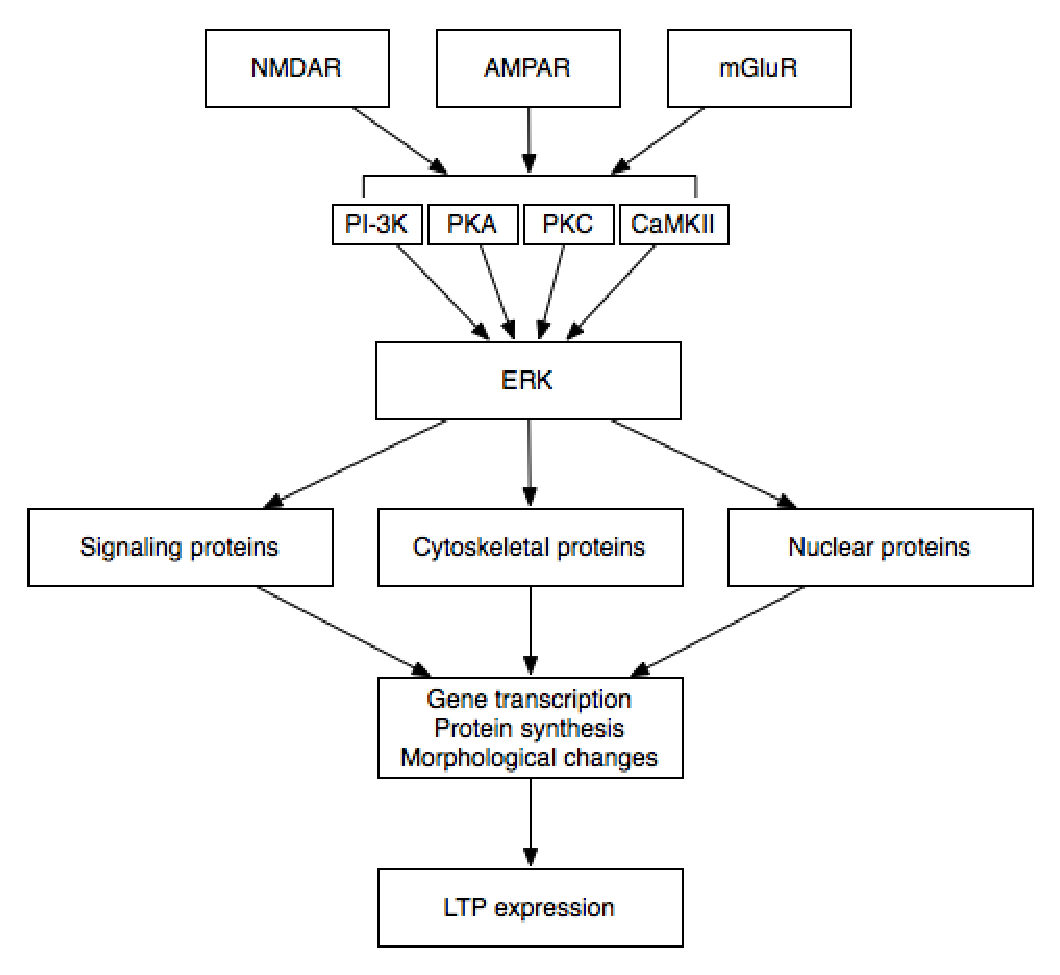
\includegraphics[height=6cm,
    angle=0]{./images/ERK_convergence.eps}}
\caption{ERK }
\label{fig:ERK_convergence}
%https://repository.library.georgetown.edu/bitstream/handle/10822/553186/janssenSchroederMeganJayne.pdf?sequence=1
\end{figure}

\subsection{ERK (classical MAPK): MAPK1/2 (ERK1/2), MAPK3 (ERK1)}
\label{sec:ERK}
\label{sec:MAPK1/2}
\label{sec:MAPK3}

Extracellular signal-regulated kinase (ERK) was originally considered equivalent
to MAPK (Sect.\ref{sec:MAPK}). Now, with more MAPK's members, ERK (representing
classical MAPK) is a member of MAPK family.
\begin{enumerate}
  \item {\bf ERK1} (MAPK3): 
  
  Transgenic gene knockout mice lacking MAPK3 are viable and it is thought that
  MAPK1 can fulfill most MAPK3 functions in most cells. Exception: MAPK3
  is important for T cells, i.e. lacking MAPK3
  reduces T cell development into CDC4+ CD8+ stage.

  \item {\bf MAPK1} is aka MAPK2: so they are often called MAPK1/2.
  Nowadays, {\bf MAPK1/2} is called as ERK1/2.
  
  MAPK1 has 85\% sequence similarity with MAPK2.
  They were found during a search for protein kinases that are rapidly
  phosphorylated after activation of cell surface tyrosine kinases such as the
  epidermal growth factor receptor (EGFR - Sect.\ref{sec:EGFR}).
  
  No conditional MAPK1 KO mouse was survived, suggesting critical functional
  role of MAPK1. 
\end{enumerate}


Depending on the cellular context, the MAPK/ERK cascade
(Sect.\ref{sec:MAPK/ERK-pathway}) mediates diverse biological functions such as
cell growth, adhesion, survival and differentiation through the regulation of
transcription, translation, cytoskeletal rearrangements. About 160 substrates
have already been discovered for ERKs.
\begin{itemize}
  \item Many of these substrates are localized in the nucleus, and seem to participate
in the regulation of transcription upon stimulation.

The substrates include transcription factors (such as ATF2, BCL6, ELK1, ERF,
FOS, HSF4 or SPZ1), cytoskeletal elements (such as CANX, CTTN, GJA1, MAP2, MAPT,
PXN, SORBS3 or STMN1), regulators of apoptosis (such as BAD, BTG2, CASP9, DAPK1,
IER3, MCL1 or PPARG), regulators of translation (such as EIF4EBP1) and a variety
of other signaling-related molecules (like ARHGEF2, FRS2 or GRB10).
  
  \item  However, other substrates are found in the cytosol as well as in other
  cellular organelles, and those are responsible for processes such as
  translation, mitosis and apoptosis. 

Protein kinases (such as RAF1, RPS6KA1/RSK1, RPS6KA3/RSK2, RPS6KA2/RSK3,
RPS6KA6/RSK4, SYK, MKNK1/MNK1, MKNK2/MNK2, RPS6KA5/MSK1, RPS6KA4/MSK2, MAPKAPK3
or MAPKAPK5) and phosphatases (such as DUSP1, DUSP4, DUSP6 or DUSP16) are other
substrates (of MAPK/ERK) which enable the propagation the MAPK/ERK signal to
additional cytosolic and nuclear targets, thereby extending the specificity of
the cascade.
\end{itemize}
\url{http://www.uniprot.org/uniprot/P27361}

As mentioned earlier, activation of MAPK/ERK molecule requires (1) removal of
auto-inhibition; (2) phosphorylation at two sites (Thr202 and Tyr-204).
Activated MAPK/ERK then can interaction with substrates.
\begin{enumerate}
  \item in the case of MAPK3 (ERK1): substrates are DUSP3, DUSP6, GTF2I, 
  HDAC4, MAP2K1, MAP2K2, PTPN7, RPS6KA2, SPIB
  
  \item in the case of MAPK1 (ERK): substrates are ADAM17, CIITA, DUSP1, DUSP22,
  DUSP3, ELK1, FHL2, HDAC4, MAP2K1, MAP3K1, MAPK14, MKNK1, Myc, NEK2, PEA15,
  PTPN17, Phosphatidylethanolamine binding protein 1, RPS6KA1, RPS6KA2, RPS6KA3,
  SORBS3, STAT5A, TNIP1, TOB1, TSC2, UBR5, VAV1.
\end{enumerate}
Dephosphorylated and inactivated by DUSP3, DUSP6 and DUSP9.

    
ERK can be the molecular link between early phase LTP to late phase LTP
(Sect.\ref{sec:LTP_depend-NMDAR}), since many signaling cascades involved in
E-LTP, including CaMKII and PKC, can converge on ERK,
Fig.\ref{fig:ERK_convergence}.
  
\begin{enumerate}
    \item ERK1: p44 MAPK
    \item ERK2: p42 MAPK
\end{enumerate}
key mediators of signal transduction from the cell surface to the nucleus. 

\subsection{atypical MAPK: ERK3 and ERK4}
\label{sec:ERK3}

atypical MAPK like ERK3 and ERK4 are two-tiered phosphorylation system, in that
they are activated by phosphorylation by PAK proteins ({\bf p21 activated
kinases}) which are related to MAP3K (Sect.\ref{sec:p21-activated-kinases}).



\subsection{MAPK/ERK-pathway: Ras-Rak-MEK-ERK pathway}
\label{sec:MAPK/ERK-pathway}

\textcolor{red}{\bf MAPK/ERK pathway}:
\begin{verbatim}
BDNF --> TrkB receptor  + EGF receptors

       ---> MAPK1/2 (or ERK1/2)
             ---> calpain-2  (NOT calpain-1)
             (
\end{verbatim}   

In neurons, MAPK1/2 (aka ERK1/2) is activated by both brain-derived neurotrophic
factor (BDNF) and EGF. Using cultured primary neurons and HEK-TrkB cells, both
of which express BDNF and EGF receptors, Jourdi et al. (2010) showed that BDNF
stimulated m-calpain but not $\mu$-calpain serine phosphorylation, and this
effect is blocked by MAPK inhibitors.

Remarkably, BDNF- and EGF-induced calpain activation was preferentially
localized in dendrites and dendritic spines of hippocampal neurons, and was
associated with actin polymerization, which was prevented by calpain inhibition.




\section{p21-activated kinases (PAK)}
\label{sec:p21-activated-kinases}

PAK (p21-activated kinases) are enzymes serve as targets for small GTP binding
protein CDC42 and Rac (Sect.\ref{sec:Rac})
\begin{enumerate}
  \item PAK1: 
  \item PAK2
  \item PAK3
  \item PAK4
  \item PAK5
  \item PAK6
\end{enumerate}

\section{CMGC group}
\label{sec:CMGC-group}

CMGC kinase group comprises a group of closely related protein kinases:
CDK (Sect.\ref{sec:CDK}), MAPK (Sect.\ref{sec:MAPK}), GSK3
(Sect.\ref{sec:GSK3}), and CLK (Sect.\ref{sec:CLK}).

They are Serine/Threonine kinases (Sect.\ref{sec:STK}).

\section{CLK}
\label{sec:CLK}



\chapter{EC3 enzymes}
\label{chap:EC3-enzymes}


Sect.\ref{sec:EC_3} describes EC3 enzyme family.
Here, we focus on a number of them.

\section{EC3: Phospholipase}
\label{sec:phospholipase}

\begin{figure}[hbt]
  \centerline{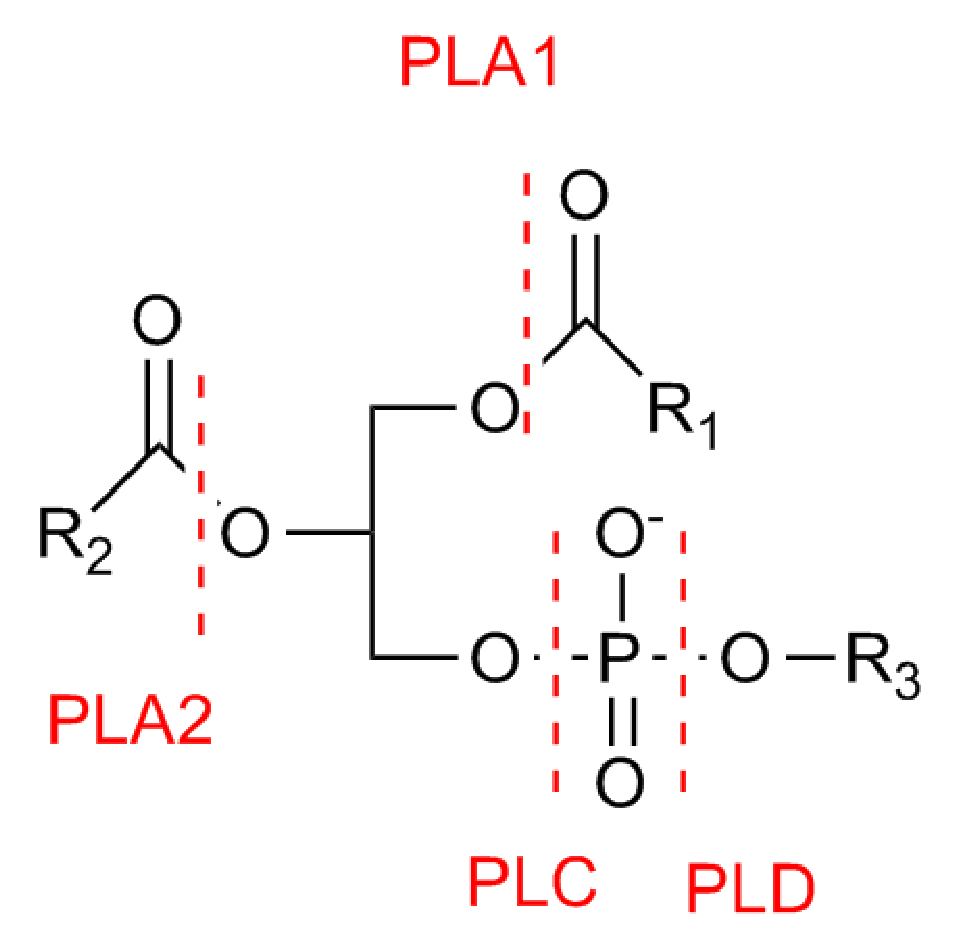
\includegraphics[height=5cm,
    angle=0]{./images/phospholipase.eps}}
\caption{Different kinds of phospholipase}
\label{fig:phospholipase}
\end{figure}


{\bf Phospholipase} is an EC 3 enzyme (Sect.\ref{sec:EC_3}) that hydrolyzes
phospholipid groups (e.g. lecithin or a similar phospholipid) of a substrate
protein. Why phospholipids is important? - Sect.\ref{sec:phospholipids}

There are 4 major classes: A, B, C, and D. 
\begin{enumerate}
  \item PLA - Sect.\ref{sec:PLA}
  
  \item PLB (EC 3.1.1.?, lysophospholipase): cleave both SN-1 and SN-2 acyl
  groups
        
  \item PLC (EC 3.1.4.3) cleaves before the phosphate
  group - Sect.\ref{sec:PLC}, release di-acylglycerol + phosphate-containing
  head group.
  
\item PLD (EC 3.1.4.4) - Sect.\ref{sec:PLD}: cleave after the phosphate group,
i.e. hydrolyze phosphatidylcholine (Sect.\ref{sec:phosphatidylcholine}) to form
phosphatidic acid (PA), releasing soluble choline to cytosol 

\end{enumerate}


PLC and PLD are considered {\bf phosphodiesterases}.
We will focus on PLC which plays an important role in signal transduction
pathways (Sect.\ref{sec:PLC}).

\section{-- phospholipase A (PLA)}
\label{sec:PLA}
\label{sec:phospholipase-A}

Phospholipase A is an enzyme that cleave phospholipid
\begin{enumerate}

   \item PLA1 (EC 3.1.1.32): cleave the SN-1 acyl group (axyl)

   \item PLA2 (EC 3.1.1.4): cleave SN-2 acyl group - Sect.\ref{sec:PLA2}
\end{enumerate}

\subsection{PLA2}
\label{sec:PLA2}

There are two PLA2
\begin{itemize}
  \item cPLA2 (85 kDa): generate arachidonic acid for signalling purpose
  
  \item sPLA2 (14-18 kDA): generate arachidonic acid for inflammatory
\end{itemize}

PLA2 is activated by ligand binding to receptors, including:
\begin{enumerate}
  \item 5-HT2 receptor (Sect.\ref{sec:5-HT_receptor})
  
  \item mGluR1
  
  \item bFGF receptor
  
  \item IFN-$\alpha$ receptor
  
  \item IFN-$\gamma$ receptor 
\end{enumerate}

Phospholipases A2 include several unrelated protein families with common
enzymatic activity.
\begin{enumerate}
  
  \item cPLA2 (85 kDA): cytosolic PLA2: $\Ca$-dependent, and involved in
  signaling process
  
  \item sPLA2 (secreated PLA2, 12-14 kDa): promote inflammation
  
  \item lp-PLA2 (lipoprotein PLA2): associated with cardiac disease
\end{enumerate}

\section{-- PLC (Phospholipase C)}
\label{sec:PLC}

{\bf PLC} (EC 3.1.4.3) is an enzyme family (class C of phospholipase -
Sect.\ref{sec:phospholipase}) whose function is to cleave the phosphate groups.
It is thus called phosphodiesterase (Sect.\ref{sec:phosphodiesterase}).
Phospholipase C is a truly remarkable signalling moiety. We know of no other
single enzyme that can produce (or modulate), directly, three distinct signals:
inositol 1,4,5- trisphosphate (IP3), diacylglycerol, and phosphatidylinositol
4,5-bisphosphate (PIP2) - Sect.\ref{sec:GPCR-PLC-IP3-DAG-pathway}. All PLC
isoforms are activated by Ca2+ ions, although their sensitivities to [Ca2+] vary
greatly (Sect.\ref{sec:PLC-Calcium}).


\subsection{3 subfamilies}
\label{sec:PLC-subfamilies}


Mammalian PLC has at least 13 isoforms, grouped into 6 subfamilies, based on
sequence similarity:
$\beta, \gamma, \delta, \varepsilon, \zeta, \eta$
~\citep{rhee2001rps,saunders2004plcz,cockcroft2006plc}.
In general, these PLC families share a conserved core architecture consisting of
an N-terminal PH domain followed by a series of EF hands, a catalytic TIM barrel
and a C2 domain, Fig.\ref{fig:PLC}.


Each isoform has a specific activator.  Depending on the subfamilies and
isoforms, they can be found in plasma membrane and/or nucleus membrane. 

\begin{enumerate}
\item {\it PLC$-\beta$}: Sect.\ref{sec:PLC-beta}
% activated by G$_{\alpha q/11}$
% subunit - Sect.\ref{sec:G-protein-coupled-receptor}

\item {\it PLC$-\gamma$}: - Sect.\ref{sec:PLC-gamma}

\item {\it PLC$-\delta$}: activated by an increase in [\ce{Ca^2+}] -
Sect.\ref{sec:PLC-delta}


\item {\it PLC$-\varepsilon$}: newly discovered in the heart, contains
  RasGEF and Ras-activated domains. - Sect.\ref{sec:PLC-epsilon}

\item {\it PLC$-\zeta$}: injected into the egg by the sperm -
Sect.\ref{sec:PLC-zeta}



\item {\it PLC-$\eta$}: Sect.\ref{sec:PLC-eta}
\end{enumerate}

% Once activated (presumbly through Gq$\alpha$ type of G protein -
% Sect.\ref{sec:Gq/11-protein}), all these first 5 types of PLC requires
% intracellular $\Ca$ to perform its catalytic function, although the optimal
% $[\Ca]$ for maximum activation is different in different PLC isozymes.
%NOTE: The residue important for Ca2+-binding is not present in PLC-beta
% isoforms.

% PLC cleaves phospholipids just before the phosphate group. An example is 
% \begin{itemize}
% \end{itemize}


% \subsection{PLC and Mg2+}
% 
% Activation of PLC-$\beta$1 by G-proteins in the presence of the nonhydrolyzable
% guanine nucleotide analogue GTP$\gamma$S was completely dependent on Mg2+ ions
% (Blank-Exton, 1991).


\subsection{PLC and Calcium}
\label{sec:PLC-Calcium}

The association of phospholipase C with Ca2+ signaling dates back arguably to
experiments published by Lowell Hokin (Hokin, 1966). 
\begin{verbatim}
PLC ---[Ca2+]--------> activated PLC
\end{verbatim}
Bob Michell suggested that inositol lipid turnover (i.e. later confirmed as PIP2
by Creba et al., 1983; Weiss et al., 1982; Berridge, 1983), initiated by
phospholipase C (PLC)-mediated inositide breakdown, was upstream of Ca2+
signaling (Michell, 1975; Michell et al., 1977). 


\begin{enumerate}
  \item Blank - Exton (1991) : PLC-$\beta$1 

Hydrolysis of PIP2 by PLC-$\beta$1 was maximal at 100$\muM$ of $\Ca$, and
calcium become inhibitory at 1 mM. 

Maximal activation of PLC-$\beta$1 (10-fold) occured between 100nM to 220nM of
calcium.
  
  \item 
\end{enumerate}

Mike Berridge (Berridge, 1983) then proposed that the released head group, IP3,
could function as a Ca2+ signaling second messenger. This was rapidly confirmed
experimentally by Berridge and his collaborators (Streb et al., 1983), and
subsequently by other investigators (Burgess et al., 1984; Prentki et al., 1984;
Joseph et al., 1984; Hirata et al., 1984; Biden et al., 1984; Whittaker \&
Irvine, 1984; Suematsu et al., 1984; Brown \& Rubin, 1984).

The less selective, Ca2+-permeable channels, the TRPCs (Sect.\ref{sec:TRPC}),
are activated by PLC, most likely by changes in membrane composition of DAG and
PIP2, Fig.\ref{fig:PLC-activated-Ca2+-influx}.
	

\subsection{PLC blockers}

\textcolor{red}{\bf PLC blockers}
\begin{enumerate}
  \item U73122 
  [1-[6-((17$\beta$-3-methoxyestra-1,3,5(10)-trien-17-yl)amino)hexyl]-1 H -
  pyrrole-2,5-dione] 5 $\muM$ applied intracellularly to block PLC-$\beta$
  
  \item 
\end{enumerate}

\subsection[PLC-beta]{PLC-$\beta$ subfamily}
\label{sec:PLC-beta}

Members of the PLC$\beta$ subfamily are composed of an N-terminal
pleckstrin homology (PH) domain, four EF-hand motifs, catalytic TIM barrel (X
and Y domains) and a C2 domain (calcium/lipid-binding domain, CaLB), and a
C-terminal coiled-coil domain (CT domain), Fig.\ref{fig:PLC}.

\begin{figure}[hbt]
  \centerline{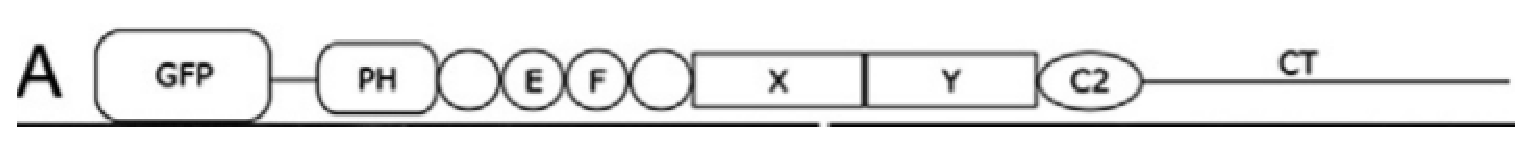
\includegraphics[height=1cm,
    angle=0]{./images/PLC.eps}}
  \caption{Core components of a PLC protein: N-terminal PH domain, 4 EF hands,
  catalytic TIM barrel (with X and Y domains), C2 domain, and C-terminal (CT)
  domain. CT domain is uniquely found in PLC-$\beta$ isozymes which is necessary
  for homodimerization and stimulation of phospholipase activity through direct
  interactions with G$\alpha$-GTP subunits of the Gq family (Sect.\ref{sec:Gq/11-protein})}
  \label{fig:PLC}
\end{figure}

Compared to other PLC subfamilies, PLC-$\beta$ has a unique long C-terminal (CT)
domain of about 450 amino acids. The EF-hand was initially proposed  to be
involved in the binding of Ca2+ ions. However, a comparison between genuine
Ca2+-binding EF hands and those of PLC$\beta$ enzymes shows that the residues
essential for Ca2+-binding are lost in PLC$\beta$ isoforms. The C2 domain does
not function as a Ca2+-binding domain either, as determined by sequence
analysis.

\subsection{-- activators}
\label{sec:PLC-activators}

Depending on the isoform, PLC$\beta$s are activated by heterotrimeric G proteins
(GTP-bound Gq$\alpha$ and/or G$\beta$$\gamma$ subunits) and/or GTP-bound Rac
(Sect.\ref{sec:PLC-beta}); and these three classes of G proteins mediate signals
originating from diverse cell surface receptors, thereby positioning PLC-b
isozymes downstream of a broad range of cellular inputs, including hormones,
growth factors and neurotransmitter.

\begin{itemize}
  \item calcium - Sect.\ref{sec:PLC-Calcium}
  
  \item G$\alpha$/q subunit bound to CT domain for activation PLC-$\beta$.
 
The Gq-selective WO82 and WO83 antiserum detected 2 types of Gq-proteins: 42kDa
and 43kDa that activate PLC-$\beta$1; which has little effect on PLC-$\gamma$ and
PLC-$\delta$ (Blank, Exton, 1991).

The activation of the 42kDa and 43kDa PLC-$\beta$1 by purified G-protein was
specific for nonhydrolyzable guanine nucleotides, the potency decreasing in the
order GTP$\gamma$S > GMPPNP > GMP-PCP. NOTE: GTP has no effect, probably
because of the intrinsic GTPase activity (GAF - Sect.\ref{sec:GAF-domain}) of
$\alpha$-subunit.

Also, activation of 42kDa and 43kDa PLC-$\beta$l by G-proteins
in the presence of GTPyS was completely dependent on Mg2+ ions with
4-5 mM proved to be optimal (Blank-Exton, 1991).
  
  \item G$\beta\gamma$ subunits also directly activate PLC-$\beta$ isozymes via
  PH domains (see below).

  \item Rac1 (target PLC $\beta$2 and $\beta$3) - Sect.\ref{sec:Rac}

NOTE: GTPase Rac1 recently found to directly activate PLC-$\beta$2 and
PLC-$\beta$3 via PH domain.
  
  PLC$\beta$2 in favor of GTPase Rac1 (over other Rho-family GTPases) :
  Rac1 engages the pleckstrin-homology (PH) domain of PLC-beta2 to optimize its
  orientation for substrate membranes (Jezyk et al. (2006))
  
 As G$\beta\gamma$ also engages the PH domain to activate PLC-beta2.
 These two activation events (G$\beta\gamma$ and Rac1) are compatible, leading
 to additive stimulation of phospholipase activity.
 
  
  \item  Waldo et al. (2010) showed that that loop between EF hands 3 and 4 of
  PLC$\beta$3 interacts with G$\alpha/q$ and promotes its GTPase activity

  \item  Another domain that is reported to interact with G$\alpha/q$ is the
C-terminal domain (CT), i.e. removal of this domain make PLC-$\beta$ no longer
activated by G$\alpha/q$ proteins. CT domains also have an inhibition effect on
calcium signaling, i.e.block the production of IP3 that is needed to trigger
internal calcium release.

CT domains derived from the various isoforms do not show a high amino acid
identity ($\approx$ 30\%).

\end{itemize}

\subsection{-- localization}

Currently, it is difficult to visualize the location of endogenous
PLC$\beta$s, since the available antibodies do not give consistent results in
immunofluorescence. Instead, VFP can be used to study.

Studying subcellular location of PLC$\beta$1a, PLC$\beta$1b, PLC$\beta$2, PLC$\beta$3,
and PLC$\beta$4a proteins was done by Adjobo-Hermans et al. (2013) 
\begin{itemize}
  \item  full-length visible-fluorescent-proteins-tagged (VFP-tagged) of these
  PLCs in Hela cells
  \item VFP-tagged of individual domains to see whether these domains play a
  role in determining the subcellular distribution of the full-length protein
\end{itemize}

They showed that
\begin{itemize}
  \item  PLC$\beta$2 and PLC$\beta$3 were not detected in the plasma membrane
 
But they must be on the plasma membrane to hydrolyze PIP3. A possible
explaination is that a minor fraction of full-length PLC$\beta$2 and PLC$\beta$3
may be localized at the plasma membrane, since such a small proportion (e.g.
10\%) is not detectable when using fluorescence microscopy.
 
Recruitment of PLC$\beta$2 and PLC$\beta$3 to membrane may be induced by
increasing the amount of PIP2 or other negatively charged phospholipids

  \item PLC$\beta$1b and PLC$\beta$4a were enriched in the plasma membrane. 

PLC$\beta$1a withouts its CT domain was not found in plasma membrane, suggesting
the important role of CT domain in anchoring the enzyme to plasma membrane.

  \item  None isoforms were found in the nucleus
  
  \item The PH domain and the C2 domain did not localize to the membrane, in
  agreement with other findings
  
  \item The CT domains of PLC$\beta$1a, PLC$\beta$1b, PLC$\beta$3
  and PLC$\beta$4a clearly locate at the membrane; yet CT domain of PLC$\beta$2
  is not. 

In addition, fluorescence level of CT$\beta$3 in cytosol also increase, as
compared to CT$\beta$1a and CT$\beta$4a.

The CT$\beta$2 was detected in cytosol, similar to CT domain in full-length
PLC$\beta$2.

\end{itemize}

\subsection{-- downstream targets}

Activated PLC-$\beta$ then slides down to hydrolyze a membrane-bound {\bf PIP2}
(Sect.\ref{sec:PIP2}), i.e.  the cleaved PIP2 turns into at least
2 second messengers - DAG (Sect.\ref{sec:DAG}) and IP3 (Sect.\ref{sec:IP3}).
\begin{itemize}
  \item DAG activate PKC (Sect.\ref{sec:PKC}) which can affect NMDAR trafficking
  via NAP (NMDAR-associated proteins which recently is belived CaMKII).
  
  \item IP3 bind to and open IP3R, releasing $\Ca$ from the ER store
\end{itemize}
However, CT domains of many PLC-beta have negative effect on the PLC-beta
signaling, i.e. the overal result is that \textcolor{blue}{effects of
CT$\beta$1a, CT$\beta$1b and CT$\beta$3 on blocking calcium signaling are
significantly different from signaling of non-transfected cell} (
The strength of inhibition of CT domain follows the decrease order: 
CT$\beta$1a  $\geq$ CT$\beta$3 $\gg$ CT$\beta$2; which is correlate with the
affinity of the CT domain to the plasma membrane) This has been explained by
 
\begin{itemize}
  
  \item  CT domain (CT$\beta$1a, CT$\beta$1b, CT$\beta$3) blocking the upstream
  effect of G$\alpha$q.

This is based on the evidence that this inhibition
can be overcome by over-expression of G$\alpha$q. 
  
  \item CT domain (CT$\beta$1a) blocking the PLC hydrolysis of PIP2.
\end{itemize}

% \textcolor{red}{However, CT domain of PLC-$\beta$1 have
% a negative effecbeen shown to produce inhibition in the PLC-$\beta$1's
% production of IP3}.

\begin{mdframed}

{\bf To understand the role of CT domains} - Two cases: non-transfected cell
with transfected cell (i.e. cell having CT domains of an associated PLC); both
with $\Ca$-indicator Fura-red (Sect.\ref{sec:fura-2}) (Adjobo-Hermans et al.,
2013). 
\begin{itemize}
  \item Histamine $\rightarrow$ 5-HT receptor activation $\rightarrow$ PKC
  activation $\rightarrow$ IP3 production $\rightarrow$ $\Ca$ release from ER 
  $\rightarrow$ free Fura-red level reduced, i.e. an increase in cytosolic
  $\Ca$.
  
  \item With the expressed CT$\beta$1a, the overal increase of cytosolic $\Ca$
  was small. 
  
  \item With the expressed CT$\beta$1b, calcium level still increase; yet with a
  significant delay 
  
The delay here is explained by inhibition of IP3 production which requires the
time to build up enough IP3 for opening IP3R to release ER $\Ca$. 

  
  \item With the expressed CT$\beta$2, calcium level still increase (yet with
  a minor delay and the elevation is somewhat smaller)
  
  \item With the expressed CT$\beta$3, calcium level increase at a smaller
  level; and with a significant delay
\end{itemize}

\end{mdframed}

\textcolor{red}{ROLE 1}: Activated PLC-$\beta$ is part of the GPCR-mediated
signaling at the plasma membrane (Sect.\ref{sec:GPCR-PLC-IP3-DAG-pathway}).
This role is important in (1) cardiovascular function, (2) neuronal plasticity.
\begin{enumerate}
  \item  hippocampal synapses, PLC$\beta$ acts as an efficient
coincidence detector triggering retrograde endocannabinoid
signalling to mediate {\it short-term plasticity}
(Hashimotodani et al. 2005, 2008).

  \item  
\end{enumerate}

\textcolor{red}{ROLE 2}: PLC-$\beta$ is also a component of a mitogen-activated
nuclear phosphoinositide signaling pathway. A large fraction of total cellular
PLC-$\beta$ can be found in the nucleus.
Mitogenic agents stimulate nuclear PLC-$\beta$ activity through a mitogen
activated protein kinase (MAPK) cascade - Sect.\ref{sec:MAPK}.

\textcolor{red}{ROLE 3}: 
\begin{itemize}
  \item PLCB1 has been shown to interact with TRPM7
  \item PLCB2 has been shown to interact with TRPM7 and MAP2K3.
  \item PLCB3 has been shown to interact with $\Na/\H$ exchange regulatory
  factor cofactor 2.
  \item PLCB4 (nothing else)
\end{itemize}


\subsection{-- Isoforms}

There are 4 major isoforms: PLC-$\beta_1$, PLC-$\beta_2$, PLC-$\beta_3$, and
PLC-$\beta_4$; each encoded by a different gene in human PLCB1, PLCB2, PLCB3,
and PLCB4, respectively. These isoforms differ in their tissue distribution,
molecular mass, specific activity, and sensitivity to regulation by G protein
subunits; suggesting that each isoform could play a divergent role in cellular
signaling (review: Adjobo-Hermans et al. (2013)).

\begin{itemize}
  \item PLC-$\beta$1: expressed at high levels in the brain.

PLC$\beta$1 is the major isozyme in hippocampal neurons.
  
\citep{dowal2008} studied on  PC12 and HEK293 cells and suggested that
activation of PLC-$\beta$1 by Gq is achieved through changes in intermolecular
interactions rather than diffusion and association. These pre-formed complexes
in turn give rise to rapid, localized signals.
  
  \item PLC-$\beta$2: expressed in cells from hematopoietic origin.
  
There are also two other modes of PLCbeta(2) membrane recruitment that
may accommodate contrasting functional needs to hydrolyze PIP2 in localized
versus dispersed populations (Sect.\ref{sec:PLC-beta}) \citep{gutman2010}.

  \item PLC-$\beta$3: ubiquitously expressed
  
  \item PLC-$\beta$4: expressed in specific parts of the brain and the retina
  
NOTE: PLC-$\beta_1$, PLC-$\beta_3$: found in most cells, albeit different
levels of expressions among the cells.
  
NOTE: PLC-$\beta_2$, PLC-$\beta_4$: found mainly in hematopoietic cells
and retina, respectively.

\end{itemize}

 
\subsection{-- PLC-beta-1 isoform}

PLC-$\beta$1 exists as two immunologically indistinguishable polypeptides of 150
and 140 kDa and is encoded in rat brain by two distinct transcripts of 5.4 and
7.2 kilobases (kb). NOTE: The 7.2 kb transcript is different from 5.4 kb
transcript by an additional 118 nucleotides located near the end of the coding
sequence and a 1738-nucleotide extension of the 3'-flanking region.

PLC-beta 1a and PLC-beta 1b correspond to the previously identified 150- and
140-kDa PLC-beta 1 enzymes, respectively
\begin{itemize}
  \item PLC-$\beta$1a: 1216-amino acid polypeptide derived from 5.4 kb
  transcript. 

  \item PLC-$\beta$1b:  1173-amino acid polypeptide derived from 7.2 kb
  transcript. NOTE: The additional 118 nucleotides gives rise to an open reading
  frame that is capable of coding PLC-$\beta$1b.

\end{itemize}
Both PLC-beta 1a and PLC-beta 1b are expressed in rat brain and C6Bu-1 glioma
cells.    PLC-beta 1a and PLC-beta 1b are derived from a single gene by
alternative RNA splicing (Bahk et al., 1994).

PLC-$\beta$1 can be activated by G$\alpha$q/11 protein -
Sect.\ref{sec:GPCR-PLC-IP3-DAG-pathway}, i.e. activated by two G-protein alpha
subunits, alpha-q and alpha-11. The C-terminal region as the segment containing
amino acid sequences required for activation by G$\alpha$q protein.
To have enough energy to activate PLC-$\beta$, $G_{\alpha q/11}$-GTP loose one
phosphate group and becomes $G_{\alpha q/11}$-GDP and finally re-binding to
GPCRs.

  
PLC$\beta_1$ (EC 3.1.4.11, 1-phosphatidyl-1D-myo-inositol
  4,5-bisphosphate) cleave PIP2 to form IP3 and DAG - Sect.\ref{sec:PIP2}.
  \textcolor{red}{ It  needs $\Ca$ as a co-factor}. 

\begin{verbatim}
PIP2 + H2O ----[enzyme: PLC-beta-1]---> IP3 + DAG 
\end{verbatim}
\begin{itemize}
  \item IP3 links to increase of $[\Ca]$ via IP3R channels Sect.\ref{sec:ip3-pathways}
  \item DAG links to increase PKC activity (Sect.\ref{sec:PKC})
\end{itemize}

% \begin{enumerate}
%   \item   
% % PLC$\beta_1$ is activated by two alpha subunits: G$_{\alpha,q}$ and
% % G$_{\alpha,11}$, or collectively called G$_{\alpha,q/11}$ which is found in 
% % mGluR1 or mGluR5 (Table \ref{tab:GPCR_ligand_Gprotein}).
% 
%    \item 
% \end{enumerate}

\subsection{-- PLC-beta-2}

PLC-$\beta$2 can be activated by 
\begin{itemize}
  \item G$\alpha$q/11 protein - Sect.\ref{sec:GPCR-PLC-IP3-DAG-pathway}

Although G$\alpha$(q) resembled Rac2 in increasing the contribution of exchange
to the FRAP of PLCbeta(2) and in enhancing its membrane association, the latter
effect was weaker than with Rac2.
 
  \item G$\beta\gamma$ protein - Sect.\ref{sec:Gbetagamma-mediate-signaling-pathway}
  
The N-terminal segment of PLC beta 2 with amino acid sequence extending to the
end of the Y box is the region required for activation by G$\beta\gamma$
\citep{wu1993}.
  \begin{itemize}
  \item G$\beta_1\gamma_1$, G$\beta_1\gamma_5$, G$\beta_2\gamma_5$ could activate
  PLC-$\beta$2 but not PLC-$\beta$1 isoform
  \item G$\beta_2\gamma_1$ does not activate PLC-$\beta$2 isoform.
\end{itemize}  
The coexpression of G$\beta_1\gamma_1$ (but not G$\beta_1\gamma_5$) and
G$\alpha$16 in COS-7 cells was able to synergistically activate PLC-$\beta$2.  


  \item Rac1 protein (Sect.\ref{sec:Rho}): Jezyk et al. (2006)
  
Rac1 engages solely the PH domain of PLC-$\beta$2 to localize and
orient it relative to substrate-containing membranes. 

\end{itemize} 

PLC$\beta_2$ (EC 3.1.4.11): similar to PLC$\beta_1$ in its catalytic function.
   
\subsection{-- PLC-beta-3}

PLC$\beta_3$ (EC 3.1.4.11): similar to PLC$\beta_1$ 

\subsection{-- PLC-beta-4}

PLC$\beta_4$ (EC 3.1.4.11): similar to PLC$\beta_1$


\subsection{PLC-delta subfamily}
\label{sec:PLC-delta}

PLC-$\delta$ is activated by an increase in [\ce{Ca^2+}].

\subsection{PLC-zeta subfamily}
\label{sec:PLC-zeta}


PLC-$\zeta$ is injected into the egg by the sperm.

\subsection{PLC-eta subfamily}
\label{sec:PLC-eta}


PLC-$\eta$

\subsection{PLC-epsilon subfamily}
\label{sec:PLC-epsilon}

PLC-$\varepsilon$ is a newly discovered PLC subfamily in the heart, contains
RasGEF and Ras-activated domains (Sect.\ref{sec:Ras}).
  

\subsection{PLC-gamma subfamily}
\label{sec:PLC-gamma}

Tyrosine kinases (Sect.\ref{sec:tyrosine}) that couple to PLCgamma; which leads
to IP3 production (Sect.\ref{sec:IP3_synthesis}).

\subsection{In hearts}

only members of the $\beta$, $\gamma$, $\delta$, $\varepsilon$
subfamilies are expressed in cardiac myocytes~\citep{berridge2003csd,
kockskamper2008ip3}.

\subsection{In neurons}
\label{sec:PLC-in-brain}


The hippocampus had the highest specific activity of PI-PLC (i.e.
phosphotidine-inositide-specific PLC), followed by striatum, frontal cortex,
cerebellum, and liver.
\begin{itemize}
  \item   aluminum chloride (AlCl3, 10-500 microM) inhibits hydrolysis of
  phosphatidylinositol 4,5-bisphosphate (PIP2) by PI-PLC in a
  concentration-dependent manner. 
  %https://www.ncbi.nlm.nih.gov/pubmed/8560464
  
  PI-PLC inhibition by 100 microM AlCl3 was greatest in the liver, followed by
  cerebellum, hippocampus, cortex, and striatum.

However, AlCl3 did not affect the shape of the calcium concentration curve,
suggesting that aluminum does not inhibit PI-PLC activity by interference with
the cofactor, calcium.
  
  \item 
\end{itemize}

Purkinje cells express all subtypes with the exception of the PLC$\beta_2$,
PLC$\beta_1$ has the lowest and PLC$\beta_4$ the highest expression level in
Purkinje cell.
\begin{itemize}
  \item PLC$\beta_3$ prevails in the caudal cerebellum
  \item PLC$\beta_4$ is reciprocally expressed in the rostral lobuli of the
  cerebellum
  
  \item PLC$\beta_1$ is present primarily in the somata of Purkinje cells and
  is, therefore, unlikely to play a major role in synaptic transmission at
  parallel fiber synapses that are all located in the spiny dendrite
\end{itemize}

PLC-beta 1 and -gamma 1, in particular, are known to protect cells from
oxidative stress.
Yasuda et al. (2008) confirmed rat cortical neurons that ER stress decreases the
expression of PLC-beta 1, but not -gamma 1, in neurons.

It is unknown whether PLC isozyme expression is affected by alteration of
intracellular Ca2+ concentration, while it is recently suggested that PLC may
have additional roles in calcium signaling, particularly in the regulation of
Ca2+ entry into cells across the plasma membrane.



\section{-- PLD (Phospholipase D)}
\label{sec:PLD}

PHospholipase D (PLD) is EC 3.1.4.4 enzyme
(Sect.\ref{sec:enzyme-classification}) that catalyze the hydrolysis,
i.e. using water to hydrolyses phosphatidylcholine
(Sect.\ref{sec:phosphatidylcholine}) into phosphatidic acid and choline.

A range of agonists acting through G protein-coupled receptors and receptor
tyrosine kinases (Sect.\ref{sec:tyrosine-kinase}) stimulate this hydrolysis. 

PLD activity has been implicated in numerous celular pathways
\begin{enumerate}
  \item signal transduction
  
  \item membrane trafficking
  
  \item regulation of mitosis
\end{enumerate} 

Isoforms: 
\begin{enumerate}
  \item Phospholipase D1 is encoded by gene {\it PLD1}
  
  \url{https://en.wikipedia.org/wiki/PLD1}
  
  \item Phospholipase D2 is encoded by gene {\it PLD2}
  
  \url{https://en.wikipedia.org/wiki/PLD2}
\end{enumerate}

\section{Protein phosphatase}
\label{sec:PP-protein-phosphatase}

A phosphatase is an enzyme that removes a phosphate group from its substrate.
This action is directly opposite to that of phosphorylases
(Sect.\ref{sec:phosphorylases}) and kinases
(Sect.\ref{sec:serine-thereonine_protein-kinases}), which attach phosphate
groups to their substrates by using energetic molecules like ATP.
\begin{enumerate}
  \item phosphorylate mGluR5 - Sect.\ref{sec:mGluR_group-1-phosphorylation}
 
Indeed, PP1$\gamma$1 (PP1C1) in both recombinant and native forms binds to the
C-terminus of long-form group I mGluRs, i.e., mGluR1a, mGluR5a, and mGluR5b
(Croci et al., 2003).
The fact that the PP1$\gamma$ 1-binding motif on mGluR1/5 falls within or
immediately distal to possible PKC phosphorylation sites (such as S881 and S890
on mGluR5a) is noteworthy. It is currently unknown whether other PP isoforms
(PP1/2A, PP2B, etc.) can directly bind to mGluR1/5.
 
  \item 
\end{enumerate}

\section{Phosphorylases}
\label{sec:phosphorylases}

A {\bf phosphorylase} is an enzyme that helps to attach phosphate groups to
their substrates by using energy.


\subsection{PP1/2A (okadaic acid-sensitive phosphatase): PP1, PP2A}
\label{sec:protein-phosphatase}

Protein phosphatases (PPs) is an enzyme that dephosphorylates an amino acid
residue of its protein substrate, i.e. removing the phosphate group. So, it
counters and balance the effect of protein kinases which add phosphate groups to
substrate (Sect.\ref{sec:protein-kinase}) - Sect.\ref{sec:phosphorylation}. 


\begin{enumerate}
  \item PP1 - Sect.\ref{sec:PP1}
  \item PP2A - Sect.\ref{sec:PP2A}
  \item PP2B - Sect.\ref{sec:PP2B}
  \item PP5
\end{enumerate}

Above proteins phosphorylate these targets
\begin{enumerate}
  \item tau - Sect.\ref{sec:tau-phosphorylation} mainly by PP2A
  
  \item CaLv1.2 (Sect.\ref{sec:CaLv1.2-channel}): PP2A and PP2B are part of the
  complex that comprises $\beta_2$ adrenergic receptor, trimeric Gs protein, AC,
cAMP-dependent protein kinase (PKA).

  \item 
\end{enumerate}


\subsection{PP1 }
\label{sec:PP1}

Protein phosphatase type-1 (PP1) includes metal-dependent protein phosphatases
(PPMs) and aspartate-based phosphatases.

Activated PP1  affects many signalling steps, by dephosphorylating receptors
such as AMPA and NMDA glutamate receptors, or GABAA receptors, voltage-gated ion
channels (Na2+, L-, and N/P-Ca2+), kinases such as calcium/calmodulin kinase II,
and transcription factors (e.g., CREB),

PP1 is inhibited by 
\begin{enumerate}
  \item phospho-Thr34-DARPP-32 (Sect.\ref{sec:DARPP32})
  
The reversed process, i.e. dephosphorylation of Thr34, is mediated by
protein phosphatase-2B (PP2B, also called calcineurin), upon activation of the
Ca2+ pathway - Sect.\ref{sec:PP2B}). 
%protein phosphatase inhibitor-1 (Sect.\ref{sec:DARPP32})
  \item 
\end{enumerate}

The inhibition of PP1 can play a critical role in disease progression.
There is a significantly lower PP1 activity in both gray and white matters in
Alzheimer disease brains.This suggests that dysfunctional phosphatases play a
role in Alzheimer's disease.

PP1 and CaMKII are mutual inhibitory [Strack et al., 1997], i.e. inhibiting PP1
would promote CaMKII activity (Sect.\ref{sec:CaMKII}).

% TODO: PP1 research more about the role of PP1 in medium-spiny neuron
%       and/or striatum.

\subsection{-- PP2A (PP2)}
\label{sec:PP2A}

Protein phosphatase 2 (PP2), also known as PP2A is a ubiquitous and conserved
{\bf serine/threonine phosphatase}.

PP2A is a dimeric enzyme composed of 3 parts:
the structural A and catalytic C subunits, and a regulatory B subunit.
There are  four classes of variable regulatory subunits: B (PR55), B' (B56 or
PR61), B'' (PR72), and B''' (PR93/PR110), with at least 16 members in these
subfamilies.


PP2A has autocatalytic dephosphorylation properties analogous to autocatalytic
kinase activity of CaMKII.
The first report of {\bf autodephosphorylation} - intermolecules self-activating
mechanism of PP2A


\subsection{PP2B (calcineurin)}
\label{sec:calcineurin}
\label{sec:PP2B}
\label{chap:calcineurin}

Calcineurin (or PP2B) is a serine/threonine proteine phosphatase
(Sect.\ref{sec:protein-phosphatase}), Fig.\ref{fig:Calcineurin_pathway}.
\begin{enumerate}
  \item a heterodimer of 2 subunits:
  \begin{itemize}
    \item calcineurin A (CnA): a 59-63 kDa (e.g. 61-kDa) calmodulin-binding
    catalytic subunit

The catalytic subunit has 3 isoforms: (in mammals) encoded by 3 different genes
(PPP3CA, PPP3CB, and PPP3CC) or ($\alpha, \beta, \gamma$).
    
    \item calcineurin B (CnB): 19-kD Ca2+-binding regulatory subunit 

The regulatory subunit has 2 isoforms: (in mammals) encoded by 2 genes (PPP3R1,
PPP3R2) or (B1 and B2).
  \end{itemize}

The name ``calcineurin'' was coined by Klee on the basis of it calcium-binding
properties and localization to neuronal tissue \citep{klee1979}. Nowadays,
Calcineurin is found to co-localize with many signaling proteins (e.g.
Ca2+/Calmodulin).
However, while CnA$\alpha$, CnA$\beta$, CnB1 gene products are found in every
cell; calcineurin CnA$\gamma$ and CnB2 expression are found mainly in brains and
testis \citep{molkentin2004cns}.

Calcineurin is CaM kinases as it is primarily regulated by $\Ca/$Calmodulin
complex and thus a major player in $\Ca$-dependent eukaryotic signal
transduction pathways (review: \citep{rusnak2000}).

   \item Cain is a 230 kDa protein with a C-terminal domain that acts as a
non-competitive inhibitor of calcineurin.

   \item AKAP79 (Sect.\ref{sec:AKAP}) is a scaffolding protein that docks
   calcineurin, PKA and PKC.

  \item Calcineurin is activated by $\Ca$, but is inhibited by cyclosporin A
(Csa)/FK506. 

To avoid many side-effect of using Csa/FK506, genetic models with inhibited
calcineurin activity were used. Strategies include: (1) overexpressing
the naturally inhibitor of calcineurin, known as {\it calcipressins} (from 2
proteins Cabin1/Cain and AKAP79), (2) transgenic overexpression of the
calcineurin inhibitory protein MCIP1 (myocyte-enriched calcineurin-interacting
protein-1), (3) dominant-negative mutant of Calcineurin, (4) Calcineurin
A$\beta$ gene targeted mice. In essnce, they used 4 separate
transgenic approach (Cain, AKAP79, MCIP1 and dnCnA) and one gene
targeted mouse model (CnA$\beta$ null) \citep{wilkins2002cac}.

\end{enumerate}



% 82, 86, 108, 171, 232, 233, 247, 267, 281, 290,
% 312, 337, 377, 397, 401, 402, 417, 441
However, the role of calcineurin in the baseline unstimulated heart is unknown.
It has been suggested that calcineurin is inactive. However, calcineurin is also
known to directly sense $[\Ca]_i$ where it is activated by sustained elevations
in intracellular calcium \citep{crabtree1999, klee1998, dolmetsch1997}.
Thus, during calcium transient, it may regulate, in part, the baseline
calcineurin activity as a mechanism for adapting cardiac load. 


Once Calcineurin is activated, it catalyses the desphosphorylation the members
of the nuclear factor of the NFAT family in the cytoplasm and promote the
translocating from cytoplasm into the nuclear where NFAT can upregulates the
expression of IL-2 (interleukin-2), Fig.\ref{fig:Calcineurin_pathway}. David Yu
Lab from JHU have showed early evidence of NFAT nuclear translocation using FRET
imaging. The suggested role of calcineurin include redox and/or oxidative
stress. In the heart, calcineurin was found to link to {\bf cardiac hypertrophy}
(Sect.\ref{sec:cardiac-hypertrophy}.



\begin{figure}[hbt]
  \centerline{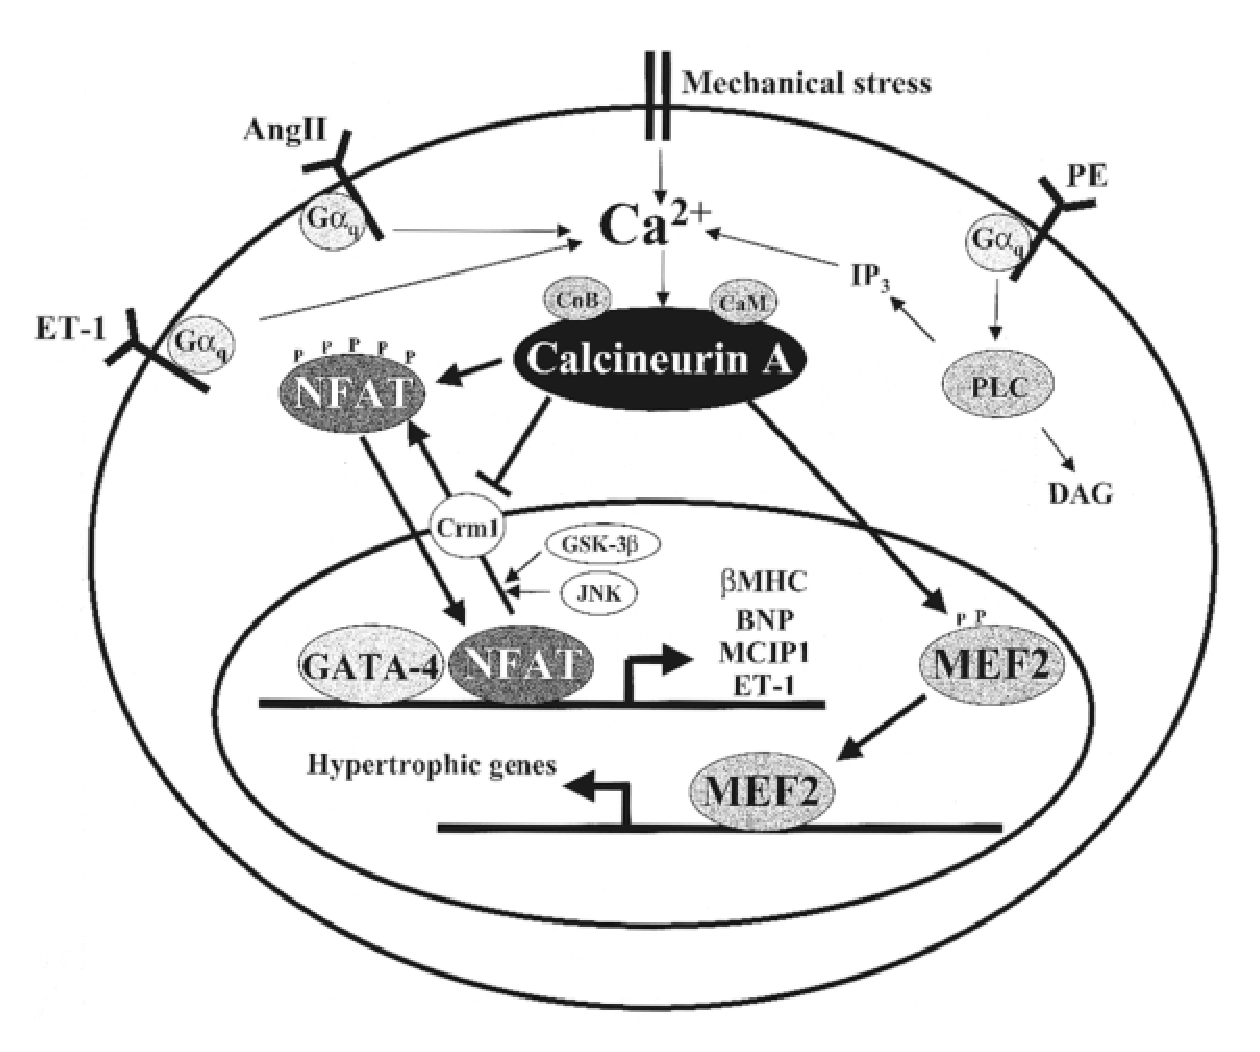
\includegraphics[height=5cm,
    angle=0]{./images/Calcineurin.eps}, 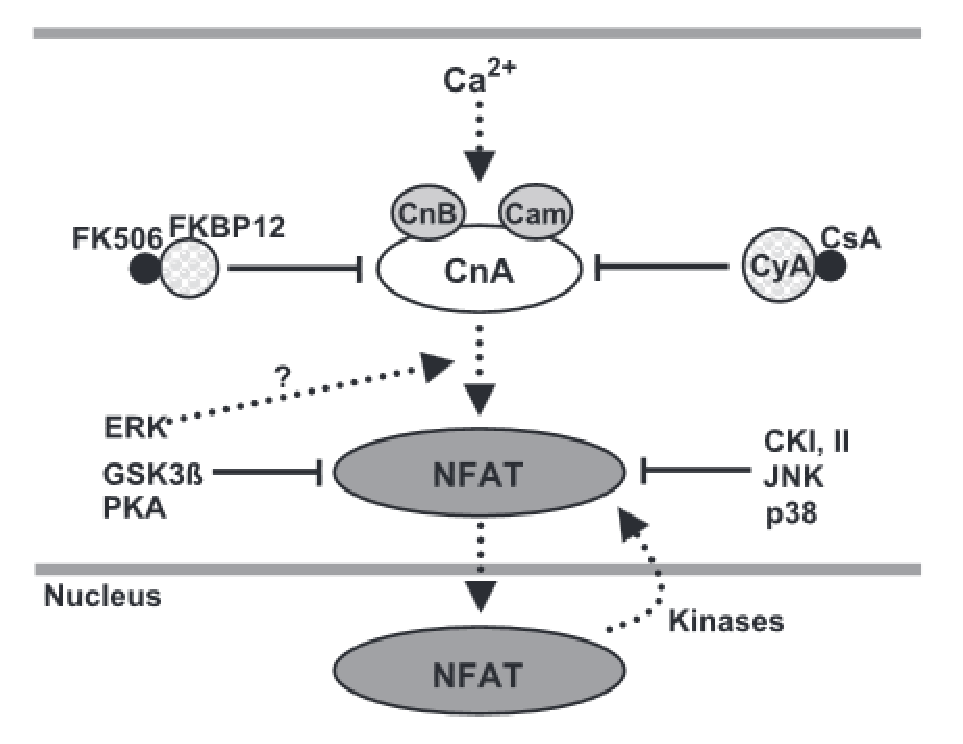
\includegraphics[height=5cm,
    angle=0]{./images/Calcineurin_2.eps}}
  \caption{Calcineurin signaling pathways in cardiac myocytes \citep{wilkins2002cac}}
  \label{fig:Calcineurin_pathway}
\end{figure}

 



\section{AKAP}
\label{sec:AKAP}

NOTE: \textcolor{red}{AKAP is a protein that can bind multiple proteins at the
same time, forming a scaffold for multi-enzyme complex} and control the
localization of such proteins.

Several AKAPs have been identified with its name given by the apparent
molecular weight on SDS-PAGE gels. AKAPs are found to localize to different
subcellular compartments, yet there quantitative distribution hasn't been
reported \citep{Yang1998}

More than 50 AKAPs have been identified, many of which are expressed in neurons
(Bauman et al., 2004; Tasken and Aandahl, 2004)
\begin{itemize}

  \item AKAP84: mitochondria

  \item AKAP220: peroxisome

  \item AKAP85: golgi

  \item MAP2: microtubules

  \item AKAP95: nucleus
  
  \item \textcolor{red}{AKAP100} tether with PKA type II
  (Sect.\ref{sec:PKA-classification}):
  
  AKAP100 localized to multiple subcellular compartments (nucleus, sarcolemma,
  intercalated disc, at Z-line region of the T-tubule and junctional SR) in
  adult rat heart with PKA type II.
  
  AKAPs bind to the N-terminal dimerization domain of PKA regulatory subunits
  and typically contain a second domain that binds to the cytoskeleton or
  intracellular scaffolds, thus targeting PKA to specific subcellular locations
  (Wong and Scott, 2004).   
\end{itemize}

\subsection{AKAP84 (in mitochondria)}
\label{sec:AKAP84}



\subsection{AKAP85 (in golgi)}
\label{sec:AKAP85}

\subsection{AKAP95 (in nucleus)}
\label{sec:AKAP95}

\subsection{AKAP100 (in neurons)}
\label{sec:AKAP100}

\subsection{AKAP220 (in peroxisome)}
\label{sec:AKAP220}

\subsection{MAP2 (in microtubules)}
\label{sec:MAP2}


\section{PDE (Phosphodiesterase)}
\label{sec:PDE}
\label{sec:phosphodiesterase}

\textcolor{red}{Review: Essayan (2001).}


3',5'-cyclic nucleotide phosphodiesterases (PDEs) refers to a family of enzyme
(Sect.\ref{sec:enzyme}) with many different PDE subtypes
(Sect.\ref{sec:PDE-classification}) that degrades cyclic nucleotide
(Sect.\ref{sec:cyclic-nucleotide}) cAMPs and cGMP
\begin{verbatim}
cAMP + H2O --------[PDE]------> 5'-AMP

cGMP + H2O --------[PDE]------> 5'-GMP 
\end{verbatim}

Catalyzation of PDE degrades cAMP and cGMP - which may disrupt normal cellular
signaling via cAMP/cGMP signaling pathways. First, you need to know the
functions of cAMP (Sect.\ref{sec:cAMP-dependent_pathway}) and cGMP
(Sect.\ref{sec:cGMP-dependent-pathways}). The downstream effects would be
cGMP-dependent protein kinase (PKG - Sect.\ref{sec:PKG}), cAMP-dependent protein
kinase (PKA) - Sect.\ref{sec:PKA}, and cAMP-regulated guanine nucleotide
exchange factors (cAMP-GEFs). 

Therefore regulation of PDEs hydrolytic activity is important for modulation of
cellular functions via PDE inhibitors (Sect.\ref{sec:PDE10-inhibitor}) which
breaks a phosphodiester bond (Sect.\ref{sec:phosphodiester-bond}) of cyclic
nucleotide (Sect.\ref{sec:cyclic-nucleotide}), i.e. cAMP and cGMP.


\subsection{classification: PDE I, PDE II, PDE III}
\label{sec:PDE-classification}

\textcolor{red}{PDE are classified into 3 classes: I, II and III}, each with
its own catalytic domain structure. We will focus on PDE I
(Sect.\ref{sec:PDE-I}) as it presents on higher level species.

\subsection{-- PDE II}
\label{sec:PDE-II}

PDE II has been  identified in slime molds, fungi, and bacteria, and contain a
distinct catalytic domain structure ({\bf PDEase II}) that is selective for cAMP
as a substrate. 

\subsection{-- PDE III}
\label{sec:PDE-III}

PDE III exist only in prokaryotes, and have a completely different catalytic
mechanism that resembles that of the purple acid phosphatases.

\subsection{PDE I: contains 11 families PDE1 - PDE11}
\label{sec:PDE-I}


Class I PDE (PDE I) is a class of PDE (Sect.\ref{sec:PDE}) that contains the
characteristic {\bf PDEase I} catalytic domain and consist of eleven distinct
families differing in substrate specificity (e.g. cAMP - Sect.\ref{sec:cAMP}),
tissue localization, regulatory mechanisms, and pharmacological properties.

Found in vertebrates, including human, rat, and mouse, Class I PDE is composed
of 21 genes, grouped into 11 families (PDE1 to PDE11) \citep{Omori2007} .
3 additional families have been reported; but not enough data (Essayan, 2001).
Five of the eleven PDE families (including the photoreceptor PDE6 family)
contain regulatory modules that have been termed GAF domains -
Sect.\ref{sec:GAF-domain}. Human has more than 50 PDE isoforms.

\textcolor{red}{NAMING CONVENTION}: hsPDE4D1
\label{sec:PDE-name-convention}
\begin{itemize}
  \item first 2 letters: indicate animal species (e.g. hs = homo sapien)
  \item PDE4 = the family; the Arabic number after PDE designate the gene
  family (1..11)

  \item D = the letter refers to the distinct subfamily gene (A..D)
  
  \item 1 = the number refers to splice-variant (isoforms); 
  each with different functional and regulatory characteristics, may exist for
  any given gene product. The splice variants in PDE regulates a specific cell
  signaling.
\end{itemize}


{\bf DETAILS}: NOTE (Km = $\muM$ = $\mu$mol/L)
\begin{enumerate}
  
  \item PDE1 (3 genes): hydrolyze both cAMP (Km=1-30) and cGMP (Km=3), expressed
  in a non-myocyte fraction of cardiac tissue, brain, lung and smooth muscle,
  activated by $\Ca$/Calmodulin, i.e. a CaM binding site (Sect.\ref{sec:calmodulin}).
  
  \item PDE2 (1 gene): hydrolyze both cAMP (Km = 50) and cGMP (Km=50), expressed
  in adrenal gland, heart, lung, liver and platelets; activated by cGMP
  binding to GAF domains - Sect.\ref{sec:GAF-domain}
  
  \item PDE3 (2 gene) - holds a trans-membrane domain: hydrolyze both cAMP (Km =
  0.2) and cGMP (Km=0.3) (yet with higher $V_\max$ for cGMP); expressed 
  heart, lung, liver, platelets, adipose tissue, and immunocytes.
  
  \item PDE4 (4 gene): specific for cAMP (Km=4); as for cGMP (Km > 3000);
  expressed in Sertoli cells, kidney, brain, liver, lung, and immunocytes
  
  It has upstream conserved regions (UCRs).
  
  \item PDE5 (1 gene): specific for cGMP (Km=1); as for cAMP (Km=150), highly
  expressed in vascular smooth muscle; and also found in lung, platelets.
  
  \item PDE6 (3 gene): specific for cGMP (Km=60); as for cAMP (Km=2000). It is
  however is a photoreceptor.
  
  \item PDE7 (2 genes): specific for cAMP (Km=0.2); as for cGMP (Km > 1000);
  expressed in skeletal muscle, heart, kidney, brain, pancreas, T lymphocytes.
  
  \item PDE8 (2 genes): specific for cAMP (Km=0.06); IBMX-insensitive;
  expressed in testes, eye, liver, skeletal muscle, heart, kidney, ovary, brain,
  T lymphocytes.

It has a response regulator receiver (REC) domain [Pfam accession
no. PF00072] and a per-arnt-sim (PAS) domain [Pfam accession no. PF00989].

  \item PDE9 (1 gene): cGMP-specific (Km=0.17), IBMX-insensitive;
  expressed Kidney, liver, lung, brain.
  
  \item PDE10 (1 gene): hydrolyze both cAMP (Km=0.05) and cGMP (Km=3.0) -
  Sect.\ref{sec:PDE10}; and expressed in Kidney, liver, lung, brain
  (specifically enriched in striatal SPN -
  Sect.\ref{sec:HD-role-of-PDE10-loss}).
  
  Inhibitors: TP-10

  \item PDE11 (1 gene): hydrolyze both cAMP (Km=0.7) and cGMP (Km=0.5); 
  expresed in skeletal muscle, prostate, kidney, liver, pituitary and salivary
  glands, testes
\end{enumerate}
Recent data showed that Phosphodiesterases (PDE)  localize to specific
subcellular, and control the temporal/spatial dynamics of cAMP, allowing a
highly localized cAMP gradients in cell. 


\begin{figure}[hbt]
 \centerline{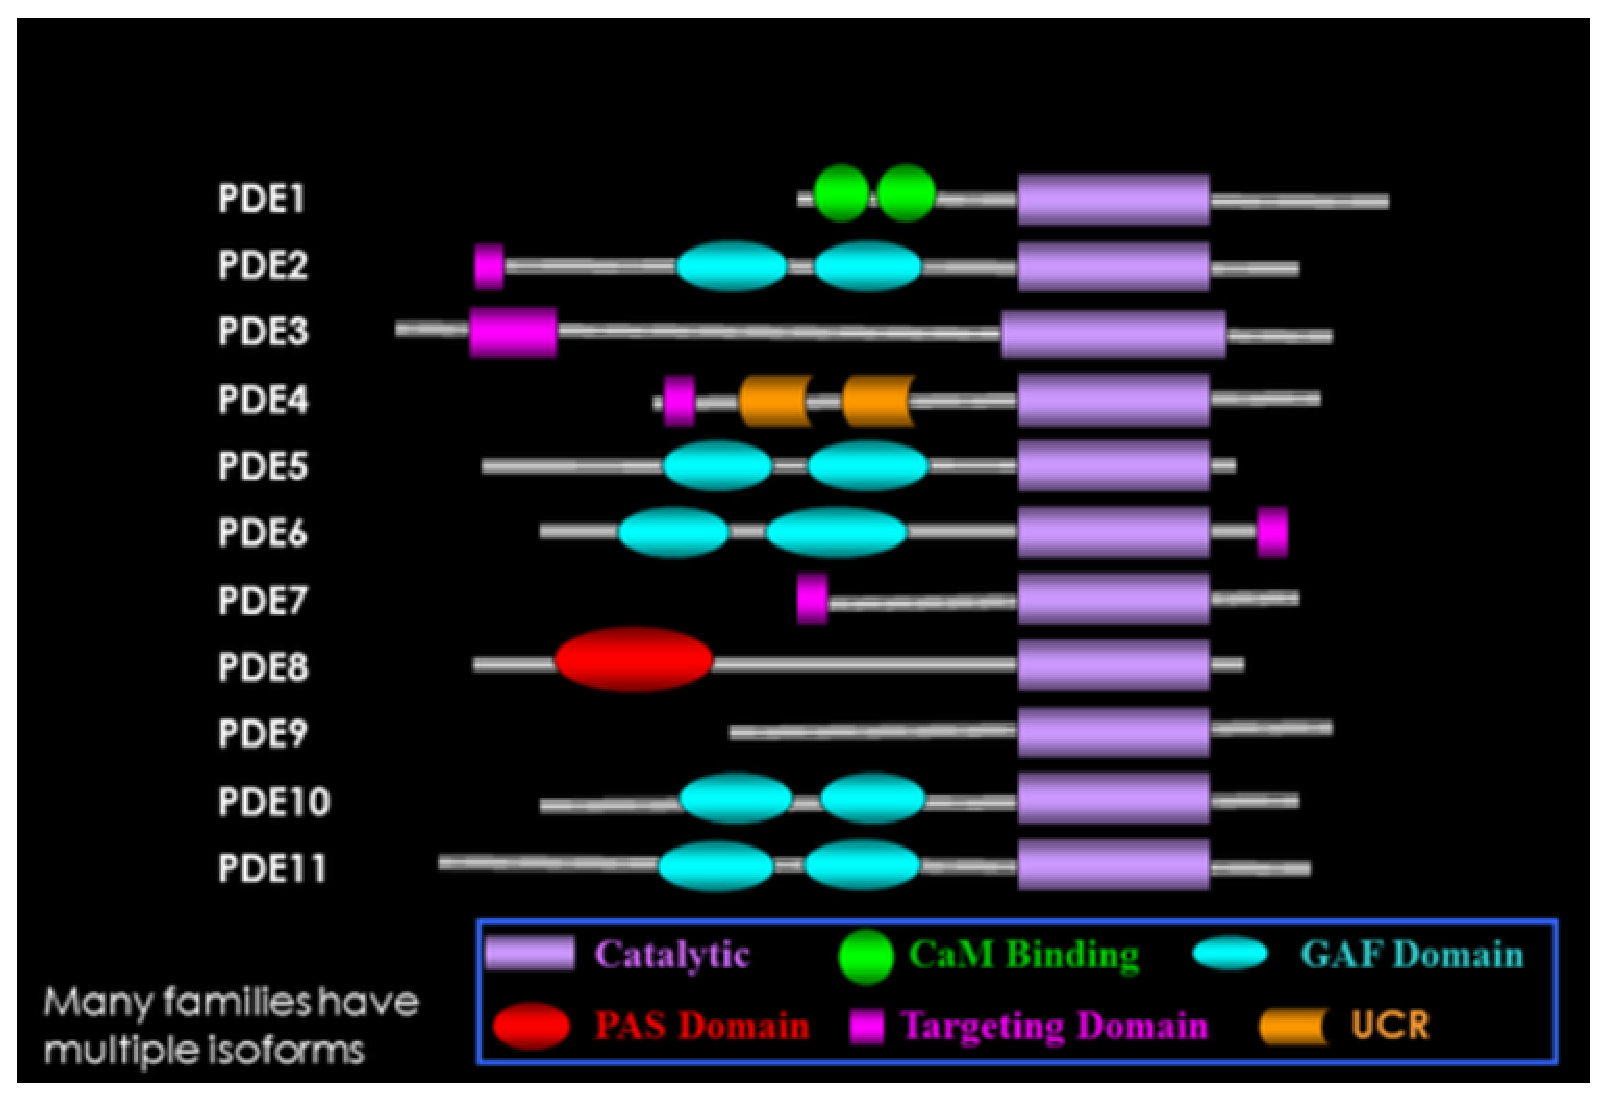
\includegraphics[height=4cm]{./images/PDE-class-I.eps}}
\caption{Structures of 11 families of PDE-class-I: left (N-terminal) to right
(C-terminal): PAS domain, CaM binding site, GAF domain}
\label{fig:PDE-class-I}
\end{figure}

\subsection{-- PDE I structure}
\label{sec:PDE-I-structure}

Structure: Fig.\ref{fig:PDE-class-I}
\begin{itemize}
  
  \item The homologous HD domain on the C-terminal controls 
  the affinity to cAMP and/or cGMP: 

All families have this; yet the differences in the amino acid sequence of the
different PDE families are known to account for the substrate specificity
(cAMP-specific, cGMP-specific, or dual-substrate).
  
  \item The N-terminal of PDE controls enzymatic activity and subcellular
  localization.

\end{itemize}


\subsection{-- PDE1}
\label{sec:PDE1}

Remeber the convention of calling PDE in Sect.\ref{sec:PDE-name-convention}.
There are three genes (A, B, C) encodes PDE1, each with a splice variant of
N-terminal region (N1, N2 and N3)
\begin{enumerate}
  \item PDE1A : high affinity to cGMP 
  
  \item PDE1B : hydrolyze cGMP with a Km value lower and a Vmax value higher
  than those for cAMP.
  
  \item PDE1C :  high affinity to both cGMP and cAMP 
\end{enumerate}


\subsection{-- PDE2}

There is only 1 gene (A)
\begin{itemize}
  \item hydrolyzes both cGMP and cAMP with similar maximal rates and relatively
  high Km values

  \item with a GAF-domain (Sect.\ref{sec:GAF-domain}), cGMP can binds to
  allosterically regulate both cAMP and cGMP signaling. 
\end{itemize}


\subsection{-- PDE3}

There are 2 genes (A, B)
\begin{itemize}
  \item both shows high affinity for both cAMP and cGMP
  
  \item A low Vmax value for cGMP compared with that for cAMP
  
  \item 
\end{itemize}

The presence of a 44-aa insert in the catalytic domain is a
unique characteristic of the PDE3 family. Another special
feature is the presence of N-terminal hydrophobic membrane
association domains (NHRs). 


\subsection{-- PDE4}
\label{sec:PDE4}

PDE4D genes encode 9 splice-variants (PDE4D1-PDE4D9) with unique amino termini
which is important for subcellular localization

\begin{itemize}
  \item PDE4D3 binds to mAKAP, creating mAKAP-PKA-PDE4D3 signalling molecule
  \citep{Dodge2001}, i.e. PKA phosphorylation increase PDE4D3 activity 2x
  \citep{Lehnart2005}

  \item  
\end{itemize}

\subsection{-- PDE6 (photoreceptor)}
\label{sec:PDE6}

PDE6 family consists of 3 genes, PDE6A (rod), PDE6B (rod), and PDE6C (cone).
 
 
 
\subsection{-- PDE10}
\label{sec:PDE10}


PDE10 is a family in PDE-class I (Sect.\ref{sec:PDE-I}), and also holds the GAF
domain (Sect.\ref{sec:GAF-domain}). As encoded by only 1 gene, PDE10 is also
called PDE10A. PDE10 controlls cell's functioning via hydrolizing cAMP and cGMP
(Sect.\ref{sec:PDE10-function}).

PDE10A is expressed in Kidney, liver, lung, brain (specifically enriched in
striatal SPN - Sect.\ref{sec:HD-role-of-PDE10-loss} where it exerts a powerful
control on striatal gene expression (Kleiman et al., 2011; Strick et al., 2010).

PDE10 level is detected using PET study with PDE10 radioligand such as
$\ce{[^3H]-PF-04831704}$ to determine PDE10 $\Bmax$, i.e.
the saturation level of radioligand binding to PDE10 reflects the current level
of PDE10. A new dedicated PET scanner, microPET, is used
for imaging small laboratory animals (Sect.\ref{sec:microPET}).
  
PDE10A is hypothesized associating with Parkinson's disease and different
neuropsychiatric disorders such as Huntington's disease, obsessive-compulsive
disorders (OCD) and schizophrenia.

\begin{enumerate}
  
  \item {\bf Parkinson's Disease}:
  
  \item {\bf Huntington's Disease}:
PDE10A is highly expressed in the striatum by medium spiny neurons (almost
exclusively), and it has been demonstrated to be involved in the regulation of
striatal signaling through the reduction of medium spiny neuronal sensitivity
towards glutamatergic excitation. Scientists think that PDE10 helps brain cells
communicate with one another and that it might be a good drug target for the
disease. PDE10 inhibitors may offer a unique way to acutely boost
hypofunctioning indirect-pathway (IP) activity in HD patients and combat
especially hyperkinesic features of motor impairment.
However, PDE10 transcript and enzyme are dramatically
reduced in HD patients, questioning whether further inhibition
of PDE10 would be beneficial in a clinical context (Ahmad
et al., 2014; Russell et al., 2014). In R6/2 and Q175 mice

\begin{enumerate}
  \item fast-pace R6/2 mice: PDE10 \Bmax declined to 36\%$\pm$5\% of WT level at
  6 weeks of R6/2 (early symptomatic); and to 15\%$\pm$2\% of WT level at 15 weeks of R6/2 (end
  stage of disease)
  
  \item slow-progressing Q175 KI mice: PDE10 \Bmax has a modest upregulation
  \begin{itemize} 

    \item 114\%$\pm$12\% of WT level at 1.5 months het-Q175; and then down to
    56\%$\pm$2\% of WT level at 8-9 months old het-Q175

    \item 120\%$\pm$05\% of WT level at 1.5 months hom-Q175; and then down to
    26\%$\pm$2\% of WT level at 8-9 months old hom-Q175
  \end{itemize}

\end{enumerate}

PDE10i TP-10 (Sect.\ref{sec:PDE10-inhibitor}) was reported to ameliorate motor
and cognitive dysfunction and improved neuropathological abnormalities in the
R6/2 HD mouse model when dosed from pre-symptomatic ages (Giampa` et al., 2010;
Giralt et al., 2013).

PDE10 inhibitors (PDE10i) are reported to enhance cortical responsivity of
iSPNs, but not dSPNs in wild-type (WT) rats (Threlfell et al., 2009) as shown
greater induction of DARPP32 phosphorylation in response to PDE10i
in iSPNs (about 6-fold) versus dSPNs (about 2-fold) (Nishi et al., 2008) -
Sect.\ref{sec:DARPP32}.

PDE10i in rodents, where PDE10i mainly phenocopy D2 antagonists (putative
activation of IP), suppressing rodent motor activity.

\end{enumerate}




% TODO: Read about PDE10 in Huntington disease
% http://en.hdbuzz.net/195

% TODO: To read
% http://www.soci.org/~/media/Files/Conference%20Downloads/2013/Young%20Chemists%20in%20Industry%202013/Harry_Mackenzie_Presentation.ashx

% TODO: HD project - mining the data available from CHDI

% TODO: Read about RDoC
%
% http://www.nimh.nih.gov/research-priorities/rdoc/research-domain-criteria-matrix.shtml

\subsection{---- function}
\label{sec:PDE10-function}

Soderling et al. (1999) described PDE10A - a dual substrate for cAMP and cGMP
(Sect.\ref{sec:cyclic-nucleotide}).
\begin{itemize}
  \item Km = 0.05 $\muM$ to hydrolize cAMP
  
  \item Km = 3.0 $\muM$ to hydrolize cGMP
\end{itemize}
But the rate for cGMP is faster, i.e. $v_\max$ ratio (cGMP/cAMP) is 4.7.

PDE10 inhibitors (PDE10i) are reported to enhance cortical responsivity of iSPNs
but not dSPNs in WT rats (Threlfell et al., 2009), which is reiterated directly
by biochemical evidence showing greater induction of DARPP32 phosphorylation in
response to PDE10i in iSPNs (~ 6 -fold) versus dSPNs (~ 2-fold) (Nishi et al.,
2008) - Sect.\ref{sec:DARPP32}, and indirectly by behavioral consequences of
PDE10i in rodents, where PDE10i mainly phenocopy D2 antagonists (putative
activation of IP), suppressing rodent motor 5 activity.

PDE10 level is studied using
\begin{enumerate}
  \item {\it ex vivo} PDE10-selective (binding) radioligand [3H]-PF-04831704
  
  \item   {\it in vivo} microPET (Sect.\ref{sec:microPET}) to evaluate PDE10
  levels using the PDE10 PET ligand [18F]MNI-659
\end{enumerate}


\subsection{---- ligand}
\label{sec:PDE10-ligand}

\begin{enumerate}
  \item  [18F]MNI-659 : a radioligand for imaging of the
PDE10A enzyme in microPET (Sect.\ref{sec:microPET})
 
  \item 
\end{enumerate}

\subsection{---- inhibitor (PDE10i)}
\label{sec:PDE10-inhibitor}

PDE10i 
\begin{enumerate}

  \item (non-selective) papaverine: (which means it also inhibit other PDE)
  
  \item (selective) TP-10
  
  \item (selective) PF-02545920 (PF-920):
  2-[4-(1-Methyl-4-pyridin-4-yl-lH-pyrazol-3-yl)-phenoxymethyl]-quinoline
  succinic acid.
  
PF-920 is a PDE10 Inhibitor that is in development at Pfizer for
Huntington's Disease and as an adjunctive treatment for Schizophrenia.

\url{https://orphandruganaut.wordpress.com/2014/06/03/orphan-drugs-pfizer-receives-fda-designation-for-huntingtons-disease/} 
 
 \item PF-04898798 (PF-798): Kd=0.8 nM for rat PDE10A; and this is >1000-fold
 selectivity over other PDEs.
\end{enumerate}

\subsection{-- in Heart}

\textcolor{red}{Cardiac PDEs fall into 5 families.}
\label{sec:PDE-heart}

In the heart, PDE4 (Sect.\ref{sec:PDE4}) is the subtype that regulates cAMP
\citep{Lehnart2005}. \citep{Dodge2001} showed that PDE4 binds to muscle A-kinase
anchoring proteins (AKAP). mAKAP colocalizes with LCC and RyR2 in cardiac muscle \citep{Ruehr2003,
Yang1998}

\subsection{-- in Brain}
\label{sec:PDE-brain}


\subsection{GTPase}
\label{sec:GTPase}

Small GTPases act as molecular switches in intracellular signaling pathways and
have many downstream targets.
GTPases are active when bound to GTP and inactive when bound to GDP, allowing
their activity to be regulated by GEFs, and the opposing GAF
(Sect.\ref{sec:GAF-domain}).

\subsection{GAF domain}
\label{sec:GAF-domain}
\label{sec:GTPase-activating-factor}

GTPase-activating factor (GAF) domain is a protein domain [Pfam accession no.
PF01590] (amino terminal allosteric regulatory sites).

It is suggested that activated PLC, beside cleaving PIP2 to produce IP3 and DAG,
also activate GAF
\begin{equation}
\ce{GAF <=>[h_f][k_f.(PLC*)] GAF*}
\end{equation}
with \verb!GAF*! (activated GAF), and \verb!PLC*! (activated PLC). Activated GAF
then can involve in providing negative feedback to G$\alpha$-GTP; by converting
to G$\alpha$-GDP
\begin{equation}
\ce{G_\alpha-GDP <=>[r_g][h_g.(GAF*)] G_\alpha-GTP}
\end{equation}
%NOTE: CT domain (Sect.\ref{sec:PLC})

Activated GAF hydrolyzes G$\alpha$-GTP which reduces PLC activation by
G$\alpha$-GTP. NOTE: An option to test purified G-protein's effect is using
nonhydrolyzable guanine nucleotides, e.g. GTP$\gamma$S.
(Sect.\ref{sec:guanine-nucleotide}).

The known functions of GAF domains are cGMP binding-mediated allosteric
regulation and dimerization of GAF-PDEs. \textcolor{red}{Several of the
GAF-containing PDEs bind cGMP at noncatalytic binding sites, resulting in
allosteric regulation of enzyme activity in the catalytic domain.}

NOTE: Some GAF domains have also been reported to bind cAMP.

GAF-PDE subfamily: PDE2, PDE5, PDE6, PDE10, and PDE11.

Other PDEs (PDE1, PDE3, PDE4, and PDE7-9) have no GAF domain and belong to the
non-GAF-PDE subfamily.


\section{Protein phosphatase inhibitor-1 (or inhibitor-1)}
\label{sec:protein-phosphatase-inhibitor-1}


{\bf Control of protein phosphorylation/dephosphorylation occurs through
regulation of protein kinase and protein phosphatase activities and is an
integral component of intracellular signal transduction.}

\subsection{inhibitor-1}
\label{sec:inhibitor-1}

Inhibitor-1 was the first endogenous molecule found to regulate protein
phosphatase activity (Huang, Glinsmann, 1976). So, protein phosphatase
inhibitor-1 is a prototypical mediator of cross-talk between protein kinases and
protein phosphatases.

Inhibitor-1 is widely expressed in mammalian tissue with highest levels
occurring in the brain, skeletal muscle, adipose, and kidney tissues.
Within the brain, the highest levels of inhibitor-1 immunoreactivity are
associated with the dentate gyrus of the hippocampus and the neostriatum and
substantia nigra of the basal ganglia. In the MSN neurons of neostriatum,
inhibitor-1 is co-expressed with a homologous PP-1 inhibitor, DARPP-32
(Sect.\ref{sec:DARPP32}); yet  inhibitor-1 is about 10 times less abundant than
DARPP-32 in the striatum.

\begin{itemize}
  \item Inhibitor-1 purified from rabbit skeletal muscle is an 18,700-kDa acid-
  and heat-stable protein composed of 166 amino acids that are highly conserved
  throughout phylogeny.
  
  \item 
\end{itemize}
% Huang F. L., Glinsmann W. H. (1976) Eur. J. Biochem. 1976:419-426. Google
% Scholar

The activation of inhibitor-1 requires it to be phosphorylated at certain sites
\begin{enumerate}
  
  \item {\bf Thr-35} by PKA: making inhibitor-1 becoming a potent inhibitor of
  PP-1 (with IC50 of 1nM - the value is dentical to that for phospho-Thr34-DARPP32)
  (Bibb, Greengard, 2001).
  The process is dephosphorylated by PP-2B and PP-2B; with PP-2B activity
  predominating in the presence of Ca2+.
  
  \item {\bf Ser-67} site (by Cdk5) in vitro: Cdk5 (Sect.\ref{sec:CDK5}) was
  found to be the only kinase that phosphorylates inhibitor-1 at Ser-67 in
  intact striatal brain tissue. The state of phosphorylation is dynamically
  regulated by NMDAR (Bibb, Greengard, 2001).
  
NOTE: phospho-Ser-67 inhibitor-1 was dephosphorylated by protein phosphatases-2A
and -2B.
    
Phosphorylation of Ser-67 did not convert inhibitor-1 into an inhibitor of
PP-1. However, it makes phospho-Ser-67 DARPP-32 becoming a less
efficient substrate for cAMP-dependent protein kinase.

\end{enumerate}



\subsection{DARPP32 (DARPP-32, PPP1R1B)}
\label{sec:DARPP32}
\label{sec:PPP1R1B}

Integration of neurotransmitter and neuromodulator signals in the striatum plays
a central role in the functions and dysfunctions of the basal ganglia. 
DARPP-32 is a key actor of this integration in the GABAergic medium-size spiny
neurons, in particular in response to dopamine and glutamate.
The name is given because of molecular weight 32 kDa (DARPP-32).
There is a homologous protein, though its level in striatal neurons is 10x less
abundant, called inhibitor-1 (Sect.\ref{sec:inhibitor-1}).


DARPP32 is a member of the so-called {\bf protein phosphatase inhibitor-1}
(Sect.\ref{sec:protein-phosphatase-inhibitor-1}). DARPP32 is both dopamine-
(Sect.\ref{sec:dopamine-signaling-pathway}) and cAMP-
(Sect.\ref{sec:cAMP}) regulated phosphoprotein.


The normal level of DARPP32 is  about 500 $\muM$ (i.e. about 10x of
inhibitor-1) (Bibb, Greengard, 2001). There are different phosphorylation sites
on DARPP32:

\begin{itemize}
  \item {\bf Thr34} (D34 form as it is presumbly via activation of D1-receptor)
  by PKA. \textcolor{red}{There are also other phosphorylation sites that
  modulate DARPP32's bility to inhibit PP-1}.
  
  cAMP-dependent protein kinase (PKA) phosphorylate DARPP-32 at the Thr34
  residue (Hemmings \& Greengard 1986; Nishi et al. 1997; Greengard et al.
  1999), presumbly via by dopamine at D1-receptor.

PKA activation requires cAMP activation (Sect.\ref{sec:cAMP}) which is
positively affected by D1-Receptor activation; and negatively affected by
D2-Receptor activation.

Upon phosphorylated at Thr34 (i.e. activation), DARPP-32 is turned into a
powerful inhibitor of the multi-functional protein phosphatase PP-1
(Sect.\ref{sec:PP1}) (with IC50 of 1nM).

Blocking PP-1 generates a series of effects on various voltage-gated and
synaptic ion channels. Because of its powerful inhibition on PP-1, DARPP32 is
also called {\bf PPP1R1B} (Protein phosphatase 1 regulatory subunit 1B), and is
one of three related, PKA-regulated inhibitors of PP1 (Sect.\ref{sec:PP1}).

  \item {\bf Thr75} site (by CDK5 - Sect.\ref{sec:CDK5}): similar to the effect
  on inhibitor-1 (Sect.\ref{sec:inhibitor-1}), this makes DARPP32 less sensitive
  to PKA.

\end{itemize}


\section{CDK: cyclin-dependent kinase}
\label{sec:CDK}

CDK belongs to CMGC group (Sect.\ref{sec:CMGC-group}). CDK involves in
regulating:  transcription, mRNA processing, and the differentiation of nerve
cells.

By definition, CDK needs a bound cyclin to function.
Without cyclin, CDK has little kinase activity; only the cyclin-CDK complex is
an active kinase. Cyclin-CDK then can phosphorylate their substrates on serines
and threonines.

NOTE: Consensus amino acid sequence
\begin{verbatim}
[S/T*]PX[K/R]
\end{verbatim}
with S/T* is the phosphorylated serine or threonine, P is proline, X is any
amino acid, K is lysine, and R is arginine.

\subsection{CDK5}
\label{sec:CDK5}

CDK5 is a cell-division protein kinase 5 that is activated by protein p35 (or
CDK5R1) and p39 (or CDK5R2); although these proteins have no cyclin sequence
homology.

\begin{enumerate}
  \item p35 \ref{sec:p35-protein}
\end{enumerate}



\section{PI3K/Akt pathways}
\label{sec:PI3K-Akt-pathways}

The PI3K/Akt signaling pathways link recptor tyrosine kinase to TOR activation,
and thereby repress autophagy (Sect.\ref{sec:autophagy-regulators}).

\subsection{Akt/protein kinase B}
\label{sec:Akt-protein-kianse-B}

{\bf Akt/protein kinase B}, a serine/threonine kinase (Sect.\ref{sec:serine-thereonine_protein-kinases})

\begin{itemize}
  \item in inactive state: locate in cytocol
  
  \item once Akt, along with 3-phosphoinositide-dependent protein kinase 1
  (PDK1), recruited by activated PIP3 (Sect.\ref{sec:PIP3} - PIP3 is activated
  once phosphorylated by PI3K - Sect.\ref{sec:PI3K}):   it translocate to
  membrane lipid bilayer.
  
  Once Akt and PDK1 are stably colocalized at membrane, the Akt activation can
  occur.    Akt is activated by phosphorylation on its two residues: Thr308 and
  Ser473 (Alessi et al., 1996) - partial activation if only at each site and full
  activation require both sites. 
  Phosphorylation at Ser473 is critical as it occurs first, before PDK1-driven
  phosphorylation at Ther308 (Scheid and Woodgett, 2003)
  
\end{itemize}

Partial activation of Akt is reflected through an increase in phosphorylation of
two downstream substrates, Forkhead (FKHR) and mammalian target of rapamycin
(mTOR), in a delayed and prolonged manner at Akt-specific phosphorylation sites


\subsection{PI3K}
\label{sec:PI3K}

{\bf Phosphoinositide 3 kinase}  (PI3K) is the enzyme that upon activation by
growth factor can 
\begin{itemize}
  
  \item phosphorylate PIP2 (Sect.\ref{sec:PIP2}) to produce PIP3
  at D3 position in the inositol ring.
  
  This is important for hippocampal LTP as PIP3 (Sect.\ref{sec:PIP3}) are
  through to regulate membrane trafficking and mediate signaling in response to
  various stimuli in many cell types.
  
  \item associated with adaptor and scaffolding proteins in postsynaptic side
  and is imlicated in the insertion of AMPAR receptors into the membrane (Man
  et al., 2003), i.e. activation of PI3K is necessary for LTP 
  \begin{enumerate}
    \item in dentate gyrus (Sect.\ref{sec:dentate_gyrus})'s granule cells:
    \item in CA1 region of hippocampus 
  \end{enumerate}
\end{itemize}

PI3K has been shown 
\begin{enumerate}
  \item activate Akt (Sect.\ref{sec:Akt-protein-kianse-B})

Two indirects downstreams  
\begin{verbatim}
Akt --> mTOR and FKHR
\end{verbatim}


  \item to interact with the MAPK / extracellular signal-regulated
kinase (ERK) pathway under certain conditions - Sect.\ref{sec:MAPK}
  \item 
\end{enumerate}

Inhibitor
\begin{enumerate}
  \item LY294002 (10$\muM$)

LY294002  blocked phosphorylation of Akt and the prolonged phosphorylation of
FKHR and mTOR

  \item 
\end{enumerate}

\section{ATPase (EC 3.6.1.3)}
\label{sec:ATPase}

Transmembrane ATPase are EC3 enzymes (Sect.\ref{chap:EC3-enzymes}) and are
important
\begin{enumerate}
  
  \item P-type ATPase - Sect.\ref{sec:P-ATPase}

Example: $\Na/\K$-ATPase - Sect.\ref{sec:NaK_pump}: maintains the cell
membrane potential.

  \item F-type ATPase - Sect.\ref{sec:F-ATPase}
  
  \item V-type ATPase - Sect.\ref{sec:V-ATpase}
  
  \item ABC (ATP binding cassette) transporter 
\end{enumerate}
CHECK: \url{https://enzyme.expasy.org/EC/3.6.1.3}

ATPase functions by hydrolyze ATP, to provide energy needed for coupling the
transport of cations across the concentration gradient across the membrane.
%ATPases are a class of enzymes that catalyze the decomposition of ATP into ADP
\begin{verbatim}
ATP --> ADP + Phosphate-ion + Energy
\end{verbatim}
and use the released energy to drive other chemical reactions.

\subsection{V-ATPase}
\label{sec:V-ATpase}


\subsection{F-ATPase (Fo/F1-ATPase): ATP synthase}
\label{sec:Fo/F1-ATPase}
\label{sec:F-ATPase}
\label{sec:ATP-synthase}


The structure of the ATP synthase enzyme which is Fo-F1-ATPase
has only recently been worked out.  {\bf F-ATPase} contains 2 domains: F0 and
F1.
\begin{itemize}
  \item Fo domain = integral in the membrane

The o in the Fo stands for oligomycin, because oligomycin is able to inhibit its
function.

  \item F1 domain = peripheral (on the side of the membrane that protons is
  moving into), i.e. to receive protons
\end{itemize}

F-ATPase is found in complex V of mitochondria (Sect.\ref{sec:complex-V-mito}).

ATP synthase enzyme functions as a sort of rotary motor, turned by the flow of
hydrogen ions through it (from inter-membrane space into the matrix), which then
powers the synthesis of ATP.


In yeast, 60\% of these proteins are in the cristae membrane while in cardiac
mitochondria, upto 94\% are found in the crista (Mannella, Lederer et al. 2013).
As the crista are non-static structures that change in shape, size and number,
it reflects the change in ATP generation by affecting the expression of
Fo/F1-ATPase. This change occurs depending on energy requirements of the cell
during normal physiological and disease conditions.
Thus, it can be established that the morphology of crista along with the densely
packed ATP-producing protein apparatus embedded on it and the overall
mitochondrial function are linked. 

Fo/F1-ATPase {\bf modulators}
\begin{enumerate}
  \item thought to be activated by mitochondrial matrix calcium 
  
Crucial to mitochondria's performance, uptake of Ca2+ occurs mainly via Ca2+
uniporter (Sect.\ref{sec:MCU}).

  \item proton gradient, i.e. mitochondrial inner membrane potential d$\Phi$.
\end{enumerate}

\subsection{P-ATPase (E1/E2-ATPase): Na/K-ATPase, H+-ATPase, Ca2+-ATPase, SERCA}
\label{sec:P-ATPase}
%\subsection{P-type ATPases}
\label{sec:P-type_ATPase}
\label{sec:E1/E2-ATPase}
\label{sec:P-ATPase}

Most members of this transporter superfamily catalyze cation uptake and/or
efflux driven by ATP hydrolysis (details is discussed in
Sect.\ref{sec:P-ATPase-classification}). P-type ATPases (or {\bf E1-E2 ATPases})
is an important class active transporter. The name comes form (1) at least 2
conformations (E1 and E2); (2) its capability to catalyze auto-phosphorylation
of the key conserved residue {\it aspartate residue} (Asp) during the pumping
cycle.
Because of two main conformation E1 and E2 (enzyme 1 and enzyme 2); so they are
also known as {\bf E1-E2 ATPases} (Sect.\ref{sec:P-ATPase-conformation}).


Examples:
\begin{enumerate}
  \item $\Na/\K$-ATPase - Sect.\ref{sec:NaK_pump}
  \item $\H$-ATPase 
  \item $\Ca$-ATPase - Sect.\ref{sec:PMCA}
  \item SERCA - Sect.\ref{sec:SERCA_pump}
\end{enumerate}



\subsection{-- Inhibitor}
\label{sec:P-ATPase-inhibitor}

A common inhibitor to all P-type pumps is $\La$. Another one is orthovanadate.

Importantly, $\La$  increases the steady-state level of phosphorylated
intermediate of $\Ca$-ATPase, but decreases that of others.

\subsection{-- distribution}
\label{sec:P-ATPase-distribution}

In erythrocyte, it's estimated about 700 molecules of $\Ca$ pump, with as least
twice the number (>1,400 molecules) for $\Na/\K$-pump. Type III ATPase (e.g.
$\H$-ATPase) is about $10^6$ molecules, and $10^5-10^6$ range for the SERCA pump
\citep{carafoli1994}.

\subsection{-- classification}
\label{sec:P-ATPase-classification}

P-type ATPases is the superfamily, with more than 32 families, with totally more
than 400 unique members (June 2007 in Swiss-Prot) \citep{bublitz2011}. 

Members of P-type ATPases can pumps a large array of cations. Based on
phylogenetic analysis, they are classified into 5 phylogenetic subfamilies,
which are then further divided into subclasses (A, B, C, etc.)
\citep{axelsen1998}. Type I (6 membrane traverses in prokaryotic cells), type II
(4 membrane traverses in eukaryotic cels). The main electrogenic P-type ATPases
are type II and III, in which type II are the most diverse
\citep{kuhlbrandt2004}.

\begin{enumerate}
  \item Type I (6-transmembrane tranverses): transport heavy metals
    ($\ce{K+}, \ce{Cu+}, \ce{Ag+}, \ce{Cu^2+}, \ce{Zn^2+}...$)

Type I are heavy metal ATPases; while type II ATPases are characterized by the
ability to transport cations of lower molecular masses ($\Na, \K, \Ca$, and
$\H$) \citep{moller1996}.

  \item Type II ($P_2$) (4-transmembrane tranverses): 4 groups
  \begin{itemize}
    
    \item Type IIa and IIb transport $\Ca$, i.e. $\Ca$-ATPase
    (Sect.\ref{sec:Ca-ATPase}):  SERCA (Sercoplasmic/Endoplasmic Reticulum
    $\Ca$-ATPases), and PMCA (Plasma Membrane $\Ca$-ATPases).
    
    \item Type IIc are Na/K-ATPase (Sect.\ref{sec:NaK_pump}), H/K-ATPase. 
    
    \item Type IId contains a few fungal ATPase
    of unknown functions.
  \end{itemize}

%\textcolor{red}{We'll discuss Type II mainly}. :


  \item Type III: plasma-membrane $\H$-ATPase (plants and fungi -
  Sect.\ref{sec:H-ATPase}), and $\Mg$-ATPase (3 bacterial species)

  \item Type IV: ATPases involving in transport of phospholypids 
  
  \item Type V: ATPase of unknown specificity
\end{enumerate}


\begin{figure}[hbt]
  \centerline{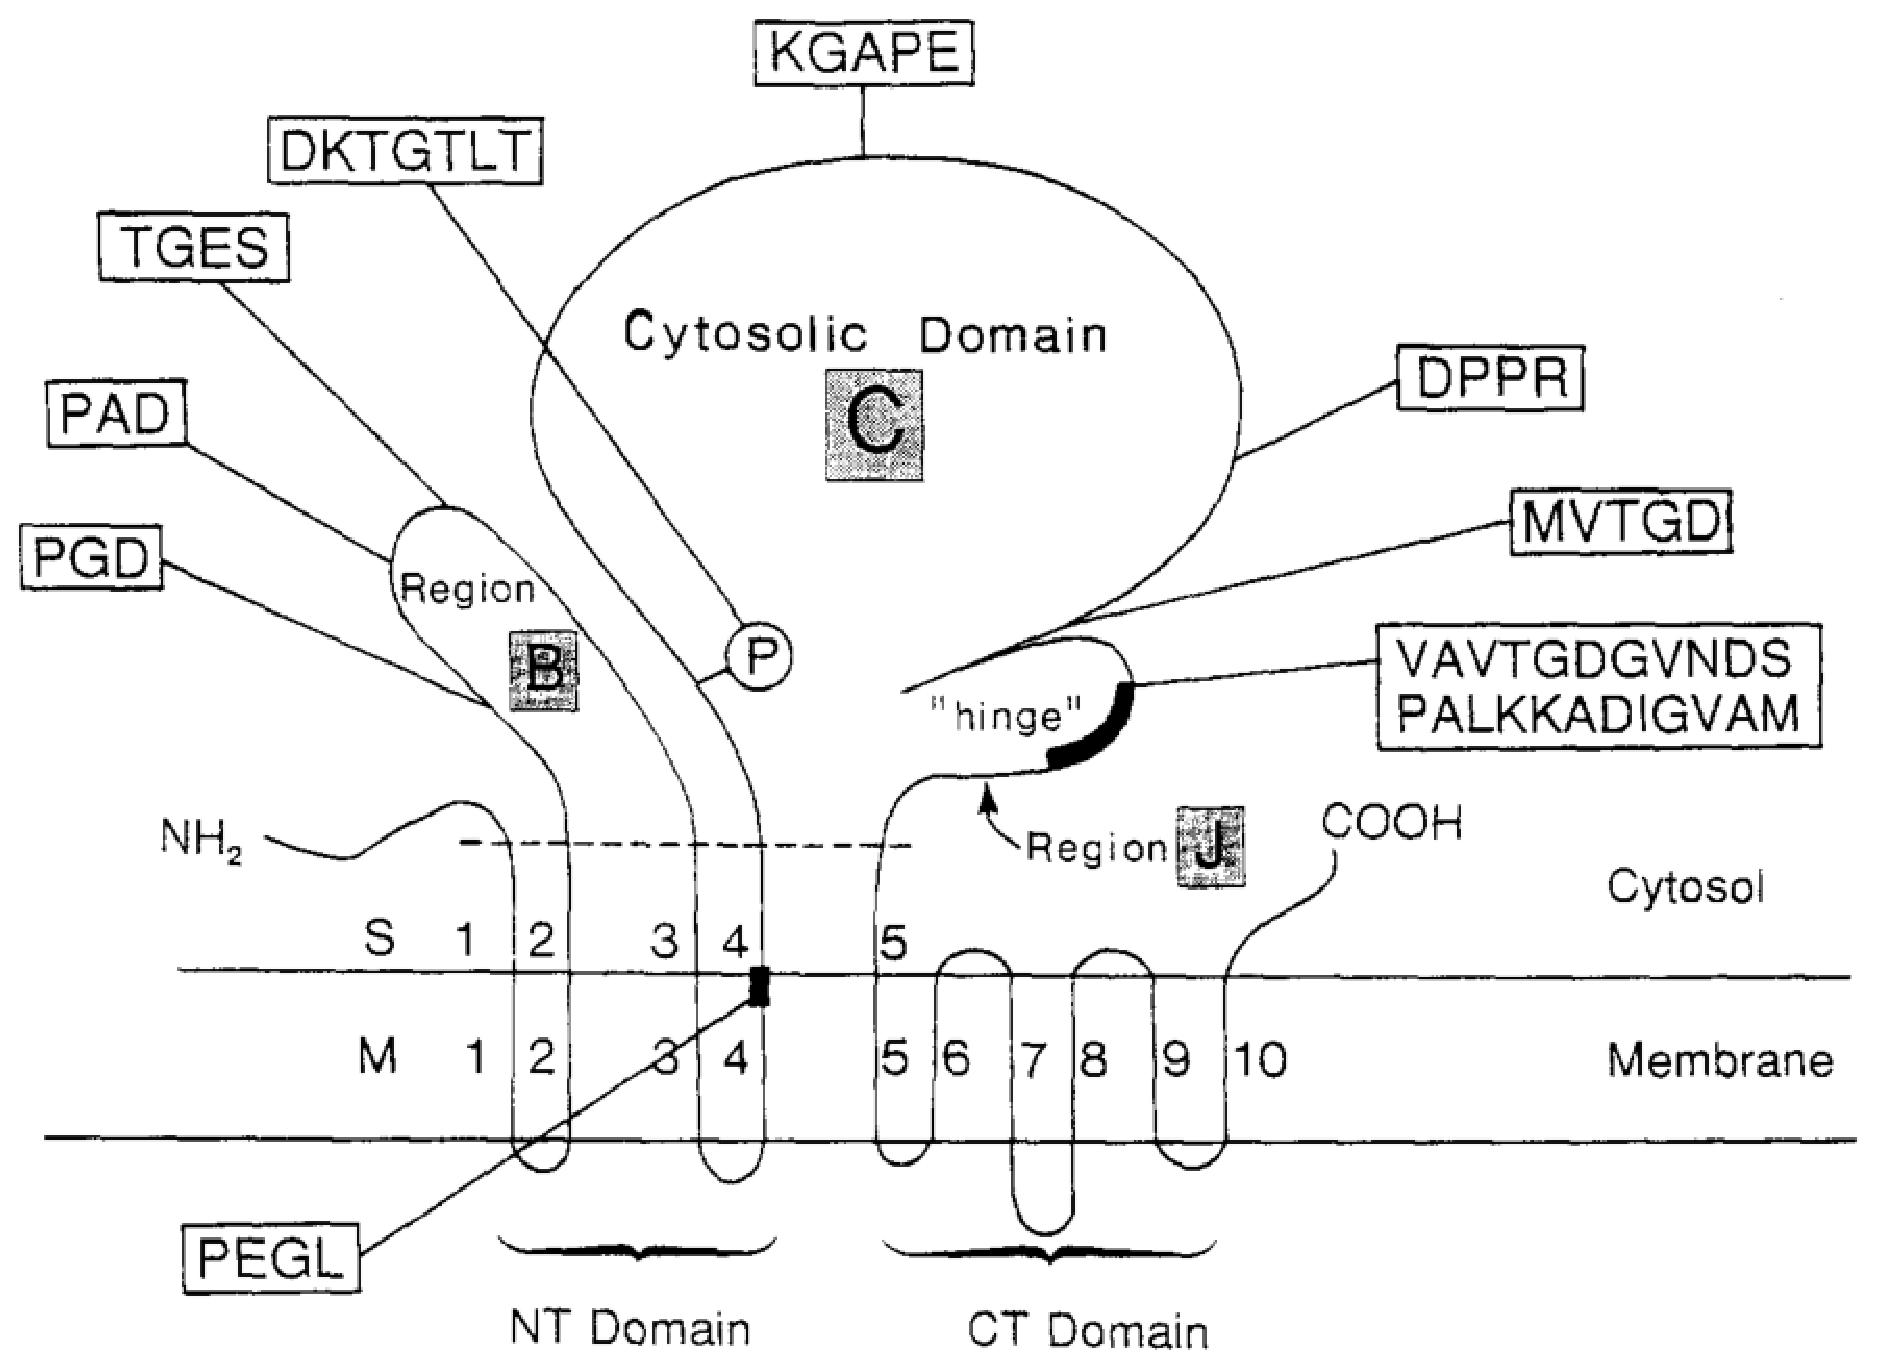
\includegraphics[height=5cm,
    angle=0]{./images/P-ATPase_type2.eps}}
\caption{Type II ATPases, represented by Na/K-ATPase \citep{moller1996}. In the
conserved region DKTGTLT, residue D is the reversibly phosphorylated Asp.}
\label{fig:P-ATPase_type2}
\end{figure}


\subsection{-- structural conformations}
\label{sec:P-ATPase-conformation}

Typically, prokaryotic P-type ATPases have lower molecular mass ($\approx
70$kDa), while eukaryotics P-type APTases have higher mass ($\approx
100-140$kDa).

Structurally, a P-type II ATPases is divided into N-terminal domain and
C-terminal domain, Fig.\ref{fig:P-ATPase_type2}. 
\begin{itemize}

  \item  N-terminal domain has 4 transmembrane helices (M1-M4), and the
  continuation of each polypeptide chain in the cytosolic side is projected as
  'stalk' segments (S1-S4).

Region B at the N-terminal part of the polypeptide chain linked to the membrane
by a number of {\it membrane traverses} \citep{moller1996}. 

  \item  C-terminal domain has 6 transmembrane helices (M5-M10). The cytosolic
  portions, comprising a 'small' and 'large' cytosolic loop, which can be
  removable by proteolytic digestion, are referred to as {\it Region B} and {\it
  Domain C}, respectively.

\end{itemize}
Domain C contains the phosphorylation site (at N-terminal end) and ATP-binding
site (in the central and C-terminal end). After the Domain C is a long stretch
of conversed sequence (known as {\it Region J}) (about 60 amino acid residues)
that connects to S5.


\begin{figure}[hbt]
    \centerline{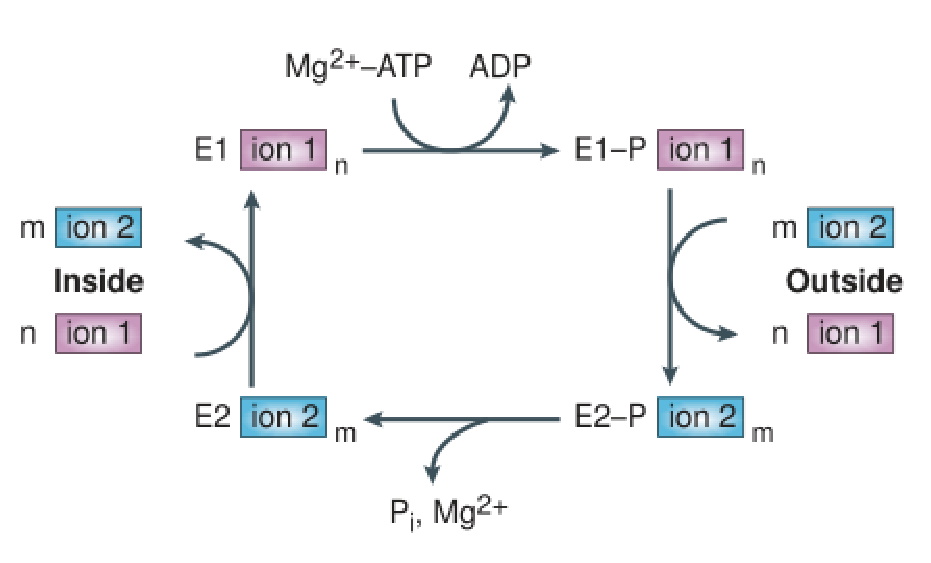
\includegraphics[height=4cm,
      angle=0]{./images/Post-Albers_cycle.eps}}
    \caption{General ion-translocation based on Post-Albers scheme
    \citep{kuhlbrandt2004}}
    \label{fig:Post-Albers-cycle}
  \end{figure}

Proteins belonging to the P-type ATPase share the conformation of an acid-stable
phosphorylated intermediate as part of its reaction cycle.
Given the above structure, typically, two major conformational state \ce{E1} and
\ce{E2} are assumed. Thus, P-ATPases are also referred to as E1/E2-ATPases.

The two states can be phosphorylated by ATP and hydrolysis Pi, respectively.
Nowadays, we know that there are other intermediate states; however, E1/E2
nomenclature is still almost universally accepted \citep{kuhlbrandt2004}. The reaction
mechanisms can be formulated in 4-step scheme, Fig.\ref{fig:Post-Albers-cycle}:
\begin{equation}
\ce{E1 ->[(1)] E1P ->[(2)] E2P ->[(3)] E2 ->[(4)] E1}
\end{equation}

In the case of Na/K-ATPase, it's called Post-Albers scheme \citep{post1972},
Fig.\ref{fig:serca_NaK_scheme}.

\begin{enumerate}

  \item Step 1: The binding of Ion1 (e.g. $\Na$ and $\K$ for Na/K-ATPase, $\Ca$
  for SER $\Ca$-ATPase) to the intracellular high-affinty site in E1 state
  triggers the phosphorylation of the enzyme by $\Mg$-ATP, resulting into the
  phosphorylated (intermediate) state \ce{E1P}. The intermediate \ce{E1P} is of
  the high-energy type, i.e. it can be dephosphorylated by ADP:
  \ce{E1P +  ADP -> ATP + \ldots}

NOTE: There are other factors that affect the rate of binding.

  \item Step 2: The translocation of the bound cations Ion1 (3Na for
  Na/K-ATPase, 2Ca for Ca-ATPase) across the membrane (from inside to outside)
  and conversion of the covalently bound  phosphate to a 'low-energy' type
  \ce{E2P}, which is unreactive with ADP. 
  
This new conformation (state) has a lower affinity to Ion1 ($\Na$ (for
Na/K-ATPase) and $\Ca$ (for Ca-ATPase)), allowing Ion1 to escape to the outside,
along with the binding of Ion2, i.e. state \ce{E2P}-Ion2.
  
  \item Step 3: Phosphate is removed from Asp residue of the enzyme by
  hydrolysis, giving the state \ce{E2} with Ion2 binding (which is $\K$ for
  $\Na/K$-ATPase, and $\H$ for $\Ca$-ATPase).
  
During this process, the terminal phosphate of ATP is transiently transferred to
aspartate (Asp) residue in the active site, resulting in reversible
conformational changes.

  \item Step 4: This step involves the translocation of other cations Ion2 (of
  2K for Na/K-ATPase, or 1-2H for Ca-ATPase) in the opposite direction. Enzyme
  returns to \ce{E1} state. This step is rate-limiting for Na/K-ATPase, where
  ATP modulation plays a crucial role for pump turnover.
  
  \item Starting a new cycle\ldots
\end{enumerate}

\begin{figure}[hbt]
  \centerline{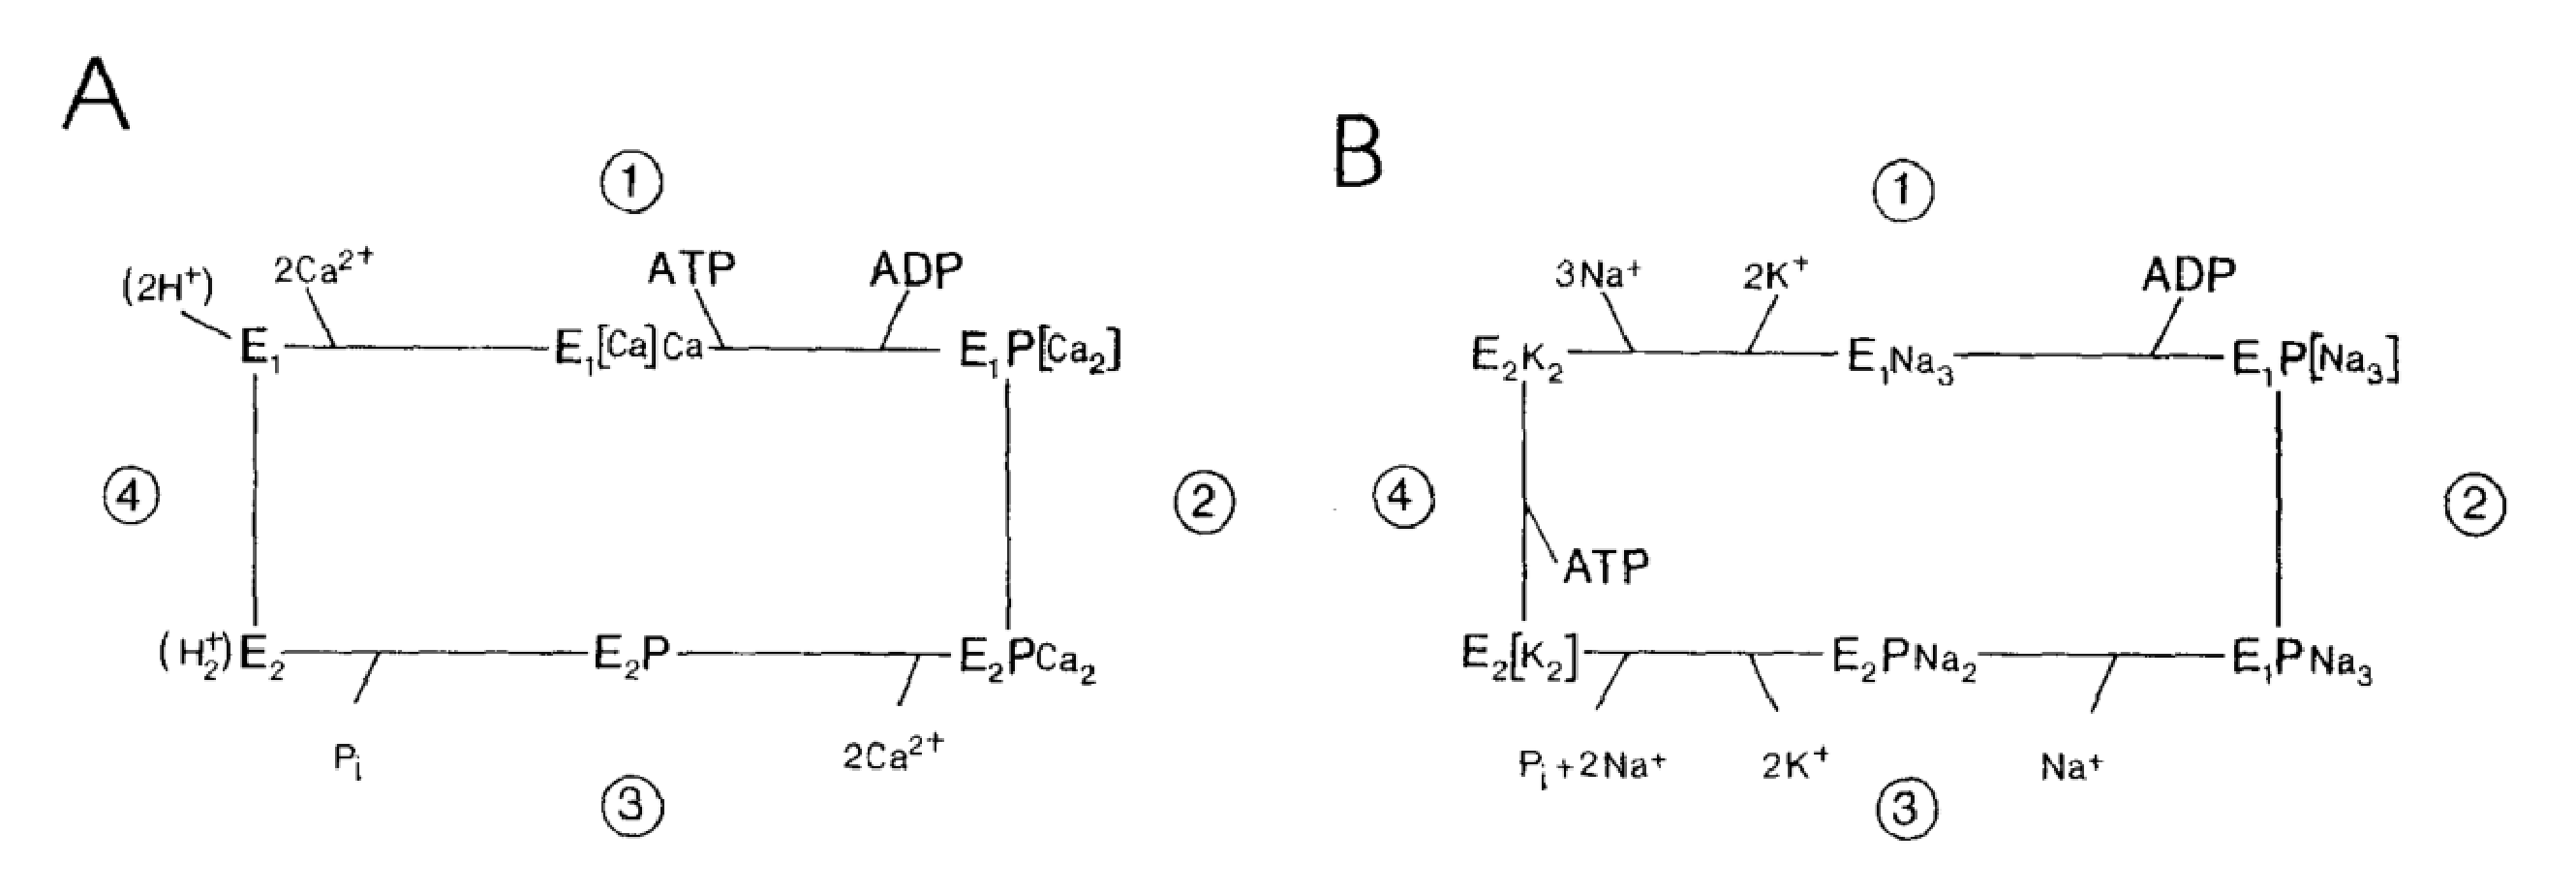
\includegraphics[height=5cm,
    angle=0]{./images/SERCA_NaK-scheme.eps}}
\caption{Kinetic scheme (A) SERCA-ATPase and (B) Na/K-ATPase \citep{moller1996}}
\label{fig:serca_NaK_scheme}
\end{figure}

Regardless of the reaction mechanism, a fundamental feature of $\Ca$ pumps is
the existence of occluded forms in steps associated with ion translocation, and
the feasibility of phosphorylation with inorganic phosphate (Pi) under \ce{E2}
state in which enzyme is unreactive with ATP or other high-energy phosphate compounds.
To stabilize the formation of transition state complex with ATPase, P-ATPases
can react with vanadate (instead of Pi). 



\subsection{AAA+ ATPase}
\label{sec:AAA+-ATPase}

{\bf Thorase} is an amino acid protein containing AAA+ ATPase domain composed of
\begin{itemize}
  \item ATP binding motif (Walker A)
  
  The mutated one is denoted as K193T or mA-Thorase.
  
  \item ATP hydrolysis motif (Walker B):
  
  The mutated one is denoted as E139Q, or mB-Thorase.
  
  \item N-linker (NL) domain: may transduce energy from ATP hydrolysis to the
rest of the protein

\item second region of homology (SRH): 
\end{itemize}

Thorase possesses ATPase activity with a $\Km$ of 43.4 $\muM$ and a $\vmax$ of
11.0 nM ATP/min/mg protein. The ATPase activity of Walker A and Walker B reduced
by 60\%-70\%, and greater than 90\%, respectively in the mutant containing both
mutations (mAB-Thorase).

Cellular distribution: Thorase is found
\begin{itemize}
  \item mainly in hippocampal CA1 pyramidal neurons
  \item at the synapse
  \item colocalize with postsynaptic marker PSD95, GluR1, and GluR2
\end{itemize}
Thorase is not expressed in axons. 



\section{Sar1}
\label{sec:Sar1}

Sar1 is a membrane trafficking protein, i

\section{Glutamate receptor-interacting protein (GRIP)}
\label{sec:GRIP}

Glutamate receptor-interacting protein (GRIP) is a family of protein binding to
glutamate receptors (Sect.\ref{sec:glutamate_receptor}), via interacting with
GluR2 subunit - a common subunit of AMPAR (Sect.\ref{sec:AMPAR}). 

\subsection{GRIP1}
\label{sec:GRIP1}

The structure of GRIP contains seven PDZ domains and binds to the C-terminus of
the GluR2 subunit of AMPA receptors (Sect.\ref{sec:AMPAR}). The AMPA receptor
amino acid sequence that the GRIP protein binds to is ESVKI (a conserved serine amino acid in the
C-terminal of both AMPAR and NMDAR).

Although the number of PDZ domains is different for the proteins PSD-95
(Sect.\ref{sec:PSD}) and GRIP, the PDZ domain is a common structural motif in
proteins that help mediate protein-protein interactions


\section{MAGUK}
\label{sec:MAGUK}

MAGUK is a superfamily of proteins: containing functional important domains:
mainly PDZ, SH3, and GUK; but many of them also contain regions homologous of
CaMKII, WW and L27 domains
\begin{enumerate}
  \item PDZ: short peptide binding sequences (80-90 amino-acids) commonly found
  at the C-terminus of interacting proteins.
  
  PDZ is an acronym combining the first letters of three proteins - post
  synaptic density protein (PSD95), Drosophila disc large tumor suppressor
  (Dlg1), and zonula occludens-1 protein (zo-1)  which were first discovered to
  share the domain.
  
  \item SH3: a protein-protein interaction domain of
  about 60 amino acids residues 
  
  They are found 
  in several other protein families such as: PI3 Kinase, Ras GTPase-activating
  protein, CDC24 and cdc25. One of the most well known features is that it can
  form an intramolecular bond with the GUK domain, creating what is known as a GUK-SH3 'closed' state.
  
  \item GUK: 
\end{enumerate} 

Members of MAGUK:  PSD95 (Sect.\ref{sec:PSD}), PSD-93, SAP97
(Sect.\ref{sec:SAP97}) and SAP102.

SAP97  and  PSD-95  can be alternatively spliced, with the $\alpha$-isoform
containing a double-cysteine/palmitoylation site, and the $\beta$-isoform having
an L27 domain at the N-terminus (Chatalov, 2009).

\begin{itemize}
  \item $\beta$-isoform of SAP97 is the most prevalent
   
  \item $\alpha$-isoform of PSD95 is the most prevalent
\end{itemize}

\section{GKAP}
\label{sec:GKAP}

guanylate kinase-associated protein (GKAP) is a family of scaffolding protein 



\section{Src-kinase}
\label{sec:Src-kinase}

Src family kinase is a family of non-receptor tyrosine kinases that include 9
members, i.e. they are not associated with cell-surface receptor:
\begin{enumerate}
  \item SrcA subfamily: Src (Sect.\ref{sec:Src}), Yes,  Fyn, and Fgr
  \item SrcB subfamily: Lck, Hck, Blk and Lyn
  \item Frn (its own subfamily)
\end{enumerate}
SrcA and SrcB subfamilies are specific to vertebrates.

\subsection{Src}
\label{sec:Src}

Src belong to SrcA subfamily of Src-kinase family (Sect.\ref{sec:Src-kinase}).
c-Src stands for "cellular Src kinase" and should not be confused with
"C-terminal Src kinase" (CSK) which is an enzyme which phosphorylates c-Src at
its C-terminus.

are not associated with a cell-surface receptor.
Src protein phosphorylates specific tyrosine residues in other proteins

Src is part of the NMDAR, Src, and Pannexin-1 complex (Sect.\ref{sec:NMDAR}).

\section{Protesome}
\label{sec:protesome}

% Cancer Treat Rev. 2003 May;29 Suppl 1:3-9.
% The proteasome: structure, function, and role in the cell.
% Adams J1.

The proteasome is a multisubunit enzyme complex that plays a central role in the
regulation of proteins that control cell-cycle progression and apoptosis, and
has therefore become an important target for anticancer therapy.

\section{STEP: striatal enriched protein tyrosine phosphatase}
\label{sec:STEP}

Striatal enriched protein tyrosine phosphatase (STEP) 
drives LTD in several ways.

\begin{enumerate}
  \item dephosphorylate the AR2 subunit of AMPAR, leading to removal of AMPAR
  from postsynaptic side
  
  \item inactivate Src by inhibiting Pyk2 (Sect.\ref{sec:Pyk2}), i.e. reducing
  Ca2+ influx via NMDAR.

NOTE: Src enhances NMDAR currents

  
\end{enumerate}

\section{Arachidonic acid (AA)}
\label{sec:arachidonic-acids}

Arachidonic acid (AA) is a polyunsaturated fatty acid present in the
phospholipids of biomembrane of cells. It is abundant in the brain, muscles, and
liver (Sect.\ref{sec:AA-production}).

AA can diffuse between cells and can act either directly or through metabolites
to alter cell functions and ionic currents (Piomelli and Greengard, 1990; Ordway
et al., 1991).

AA is a second messenger that is involved in regulation of signaling enzymes,
such as PLC-$\gamma$, PLC-$\delta$, and PKC-$\alpha$, and -$\beta$
isoforms; modulate synaptic transmission. 

The concentration at which AA occurs in tissues and cells is low: 2$\muM$
nonesterified arachidonate in the arterial blood of dogs (see Table 2 of Van der
Vusse et al., 1982), 9 - 16 $\muM$ in the plasma of rats (see Table 1 of Rapoport,
2003) and 5.3 - 13.1 $\muM$ in human plasma (see Burtis et al., 2006).
Much higher concentrations are found in secretagogue-stimulated pancreatic
islets; increments in cellular levels of 38 - 75 $\muM$ are reported by Wolf et
al. (1991). A total of 99.9\% of the non-esterified arachidonate is bound to
albumin. Therefore, the effects of fairly low (2 - 10 $\muM$) AA concentrations are of
particular interest.

It is important to distinguish between effects of AA itself and effects of AA
metabolites (Meves, 2008). Recently, the interest to functional role of AA has
been shifted from classical ion channels ($\Ca$, $\Na$ channels) to new types of
channels (TRP and non-SOCE channels).

\begin{enumerate}
  \item inhibits \textcolor{red}{HVA $\Ca$ channels} through free radical
  formation and PKC activatin (Keyser and Alger, 1990)
  
  \item either depress or enhance $\K$ current via lipoxygenase or
  cyclooxygenase metabolites (Keyser and Alger, 1990; Schweitzer et al., 1990;
  Zona et al., 1993): activate $\K$ channels in smooth muscle cell (Ordway et
  al., 1989), in cardiac muscle cells (Kim and Clapham, 1989).
 
In Aplysia, lipoxygenase metabolites of AA modulate S-type K+ channels (Piomelli
et al., 1987).

   \item enhance \textcolor{red}{NMDA-activated currents} (Miller et al., 1992).
   
   \item depress $\Na$ current in squid giant axon (Takenaka et al.,
1988) when AA at high concentration (ED$_{50}=0.18$ mM). 

In CONTROL: GABA release is induced by high $[\K]_o$ (56 mM, which activate
$\Ca$ channels) or veratrine (5 $\mu$g/ml) - which depolarize neurons by greatly
prolonging open times of $\Na$ channels (Barnes and Hille, 1988; Catterall,
1992).
AA diminished veratrine- but not K+-evoked release of [$^3$H]GABA suggests the
actions of AA on Na+ influx.

Fraser, MacVicar (1993) showed that AA 10 $\muM$ reversibly depressed the
amplitudeof INa, at all potentials (reduce 33\% at -10mV) in cultured neurons,
and reduce 30\% in acutely isolated neurons.

In Na+ channels of rat skeletal muscle, half inhibition occurs at 4 $\muM$ AA
(Bendahhou et al., 1997).

   \item modulate synaptic transmission in a complex way:
   AA enhances transmitter release at high concentrations (Freeman et al., 1990;
   Lynch and Voss, 1990) and inhibits at lower concentrations (Herrero et al.,
   1991).

A bidirectional action has been recently proposed for another intercellular
messenger, nitric oxide (Sect.\ref{sec:nitric-oxide}), which can play a positive
(Schuman and Madison, 1991) or negative (Izumi et al., 1992) role in regulating
long-term potentiation.

In striatal neurons, AA may affects the release of GABA from cultured striatal
neurons and acutely isolated striatal neurons (Fraser, MacVicar, 1993).
 
   \item TRP channels (Sect.\ref{sec:TRP-structure})
   
   \item SOCE channels (Sect.\ref{sec:SOC}) 
   
   \item non-SOCE channels:  
\end{enumerate}

\subsection{AA production}
\label{sec:AA-production}
\label{sec:arachidonic-acids-production}

Several neurotransmitters cause the release of AA by acting through
phospholipase A2 (Axelrod, 1990; Shimizu and Wolfe, 1990)

Arachidonic acid is a 20-carbon omega-6 poly-unsaturated fatty acid.
AA is freed from membrane phospholipid molecule by the enzyme
phospholipase A2 (PLA2 - Sect.\ref{sec:PLA2}), or can also be generated from DAG
(Sect.\ref{sec:DAG}) by diacylglycerol lipase (DAG lipase).
\begin{verbatim}
DAG lipase ---[cleave off DAG]----> arachidonic acid 
\end{verbatim}



\section{Nitric oxide (NO)}
\label{sec:nitric-oxide}

Nitric oxide (NO), the smallest signalling molecule known, is produced by three
isoforms of NO synthase (NOS; EC 1.14.13.39) - Sect.\ref{sec:NO-synthase}.

{\bf Nitric oxide}, a freely diffusible gas, is produced by
\begin{itemize}
  \item  several metabolic pathways in the mitochondrion and in the surrounding
  cell and has widespread effects on mitochondrial function either as NO,  or
  following conversion to peroxynitrite (\ce{ONOO^-}), or other reactive
  nitrogen species (RNS). 
  
  The precise metabolic pathways are controversial (Lacza 2009). 
\url{https://www.ncbi.nlm.nih.gov/pmc/articles/PMC4570492/}

Nonetheless, some, but not all, studies have provided evidence indicating that a
mitochondrial variant, named mtNOS, may be present in the inner mitochondrial
membrane or matrix.  

conventional NOS isoforms may be associated with the outer mitochondrial
membrane and represent an alternative, externally regulated source of NO to the
interior of the mitochondria (see next item). 

  \item 3 isoforms of NOS - Sect.\ref{sec:NO-synthase} nNOS, iNOS, eNOS.
  
  These enzymes convert L-arginine to NO and L-citrulline
  
\end{itemize}

Once formed, NO can diffuse into mitochondria from the surrounding cellular
space or could traverse longer distances from other, more remote cells.
\textcolor{red}{Remarkably, nanomolar concentrations of NO can inhibit
mitochondrial respiration, so even a small amount of NO in the mitochondrial
matrix may regulate ATP synthesis.}
\url{https://www.ncbi.nlm.nih.gov/pubmed/16051505/}


Similar to AA (Sect.\ref{sec:arachidonic-acids}), a bidirectional action has
been recently proposed for another intercellular messenger, nitric oxide
(Sect.\ref{sec:nitric-oxide}), which can play a positive (Schuman and Madison,
1991) or negative (Izumi et al., 1992) role in regulating long-term
potentiation.



\section{Tyrosine receptor kinase (Trk)}
\label{sec:Trk}

Trk are  transmembrane proteins and are receptors of neurotrophin
(Sect.\ref{sec:neurotrophin}).
Upon binding of a proper neurotrophin, Trk member then can activate many
intracellular signaling pathways, including those controlled by Ras, the
Cdc42/Rac/RhoG protein family, MAPK, PI3K and PLC-gamma.

Several novel signaling pathways controlled by Trk receptors have been
characterized, and it has become clear that membrane transport and sorting
controls Trk-receptor-mediated signaling because key intermediates are
{\bf localized to different membrane compartments}.

Differential splicing also generates an isoform of TrkC with a modified kinase
domain that has altered substrate specificity, and isoforms of TrkB and TrkC
that lack kinase domains.

A second signal, such as cAMP or Ca2+ (Sect.\ref{sec:calcium-function}), is
required for efficient insertion of receptors into the surface membrane.

\subsection{Trk-A}
\label{sec:Trk-A}

Trk-A is the receptor of NGF (Sect.\ref{sec:NGF})

Ubiquitination is a reversible post-translational modification involved in a
plethora of different physiological function. Among the substrates that are
ubiquitinated, neurotrophin receptors (TrkA, TrkB, TrkC, and p75NTR) have been
studied recently. TrkA is the most studied receptor in terms of its
ubiquitination. Sect.\ref{sec:ubiquitin} discusses ubiquitin.


\subsection{Trk-B}
\label{sec:Trk-B}

The receptor tyrosine kinase TrkB (also known as NTRK2) is the receptor of
neurotrophin BDNF (Sect.\ref{sec:BDNF}). Differential splicing also generates an
isoform of TrkB  that lack kinase domains.

TrkB is known primarily for its function during PNS and CNS development, has
emerged in recent years as a potent regulator of hippocampal LTP. Understanding
the mechanisms that underlie learning is one of the most fascinating and central
aims of neurobiological research. Hippocampal long-term potentiation (LTP) is
widely regarded as a prime candidate for the cellular mechanism of learning
(review: Minichiello, 2009)

The phosphorylation of striatal TrkBRs occurs in response to
depolarization-induced release of BDNF by cortical terminals.

\subsection{Trk-C}
\label{sec:Trk-C}

Trk-C is the receptor of neurotrophin NT-3 (Sect.\ref{sec:NT-3})

Differential splicing also generates an isoform of TrkC with a modified kinase
domain that has altered substrate specificity, and isoforms of TrkB and TrkC
that lack kinase domains.


%%% Local Variables: 
%%% mode: latex
%%% TeX-master: "mainfile"
%%% End: 

\section{Amyloid-beta}
\label{sec:amyloid-beta}

The level of A$\beta$ plaque can be detected using a sensitive sandwich ELISA
system (Green et al., 2008).

A$\beta_{1-40}$

A$\beta_{1-42}$


\section{MAP: microtubule-associated protein}
\label{sec:MAP}

Tau (Sect.\ref{sec:tau-protein}) is the major microtubule associated protein
(MAP) of a mature neuron.  The other two neuronal MAPs are MAP1
(Sect.\ref{sec:MAP1}) and MAP2 (Sect.\ref{sec:MAP2}).

\subsection{MAP1}
\label{sec:MAP1}

\subsection{MAP2}
\label{sec:MAP2} 




\subsection{tau protein: MAPT gene}
\label{sec:tau-protein}
\label{sec:MAPT-gene}
\label{sec:tau}

Tau proteins are proteins that perform the function of stabilizing microtubules.
Tau proteins belong to the microtubule-associated proteins (MAP) family -
Sect.\ref{sec:MAP}. The proteins work together with a globular protein called
{\bf tubulin} to stabilize microtubules and aid the assembly of tubulin in the
microtubules. Tau proteins - as a phosphoprotein - achieve their control of
microtubule stability through its different isoforms and phosphorylation state
(Sect.\ref{sec:tau-phosphorylation}).

These proteins are abundant in nerve cells and are present to a much lesser
degree in oligodendrocytes and astrocytes.

IMPORTANT (SUBCELLULAR-LOCATION): Tau proteins are \textcolor{red}{mainly active
in the distal portions of axons} where they stabilize microtubules as well as
providing flexibility.

Tau proteins are produced through alternative splicing of a single gene called
MAPT ({\bf microtubule-associated protein tau}). The proteins were discovered in
Marc Kirschner's laboratory at Princeton University in 1975.

The proteins work together with a globular protein called tubulin to stabilize
microtubules and aid the assembly of tubulin in the microtubules. 

\subsection{-- phosphorylation of tau protein}
\label{sec:tau-phosphorylation}

Hyperphosphorylation of tau depresses the biological activity of tau
(Sect.\ref{sec:tau}). So dephosphorylation may contribute to the disease
progression.  The four phosphatases (PP1, PP2A, PP2B and PP5 -
Sect.\ref{sec:protein-phosphatase}) all dephosphorylated tau at Ser199, Ser202,
Thr205, Thr212, Ser214, Ser235, Ser262, Ser396, Ser404 and Ser409, but with
different efficiencies toward different sites.

High levels of the serine/threonine PPases are found throughout the
brain, with PP1, PP2A, PP2B, and PP5 being abundant and implicated in AD.

\begin{itemize}
  \item  The K(m) values of tau dephosphorylation catalysed by PP1, PP2A and PP5
  were 8-12 $\muM$, similar to the intraneuronal tau concentration of human
  brain, whereas the K(m) of PP2B was fivefold higher. 
  
  \item PP2A is the major tau phosphatase that regulates its phosphorylation at
  multiple sites in human brain (Liu, Gong, 2005).
  
PP2A, PP1, PP5 and PP2B accounted for approximately 71\%, approximately 11\%,
approximately 10\% and approximately 7\%, respectively, of the total tau
phosphatase activity of human brain. 

The total phosphatase activity and the activities of PP2A and PP5 toward tau
were significantly decreased, whereas that of PP2B was increased in AD brain.

\end{itemize}


\subsection{-- tauopathies}
\label{sec:tauopathies}

Neurological disorders related to dysfunction of tau proteins are called {\bf 
tauopathies} (Sergeant et al., 2005). Many etiological factors,
phosphorylation, splicing, and mutations, relate Tau proteins to neurodegeneration.
\textcolor{red}{Normal adult human brain tau contains 2-3 moles phosphate/mole
of tau protein.}
Abnormally hyperphosphorylated tau is a key feature of human tauopathies.
Although we are not sure whether phosphorylation rather than oligomerization of
tau (Sect.\ref{sec:tau-oligomers}) is an initial molecular event in tau
pathogenesis

\begin{itemize}
  \item  AD (Sect.\ref{sec:tau-Alzheimer}): hyperphosphorylated tau proteins.
  

In Alzheimer disease (AD) brain tau is $\tilde{}$ three to four-fold more
hyperphosphorylated than the normal adult brain tau and in this
hyperphosphorylated state it is polymerized into paired helical filaments
([PHF]) admixed with straight filaments (SF) forming neurofibrillary tangles.

Some research suggests that an exosome-based mechanism may be responsible for
the release of tau proteins in Alzheimer's disease. 

\item 
\end{itemize}


\subsection{-- properties}

Tau protein has several unique characteristics such as natively unfolded
conformation, thermo-stability, acid-stability, and capability of
post-translational modifications.


\subsection{-- biomarkers}

$^{18}$F-THK523 as a tauopathy marker, i.e.
binds specifically to tau tangles.

\subsection{-- tau oligomers: NFT}
\label{sec:tau-oligomers}
\label{sec:NFT}

We still do not know whether tau itself is toxic. 

Researchers are now looking for 'tau oligomers' as toxic components, because
'tau oligomers' contain variable species of tau protein [e.g., dimer (disulfide
bond-dependent or -independent), multimer (more than dimer), granular (defined
as EM or AFM) and perhaps small filamentous aggregates ] (Sahara, Avila, 2014).

{\bf Neurofibrillary Tangles} (NFTs) are aggregates of hyperphosphorylated tau
protein that are most commonly known as a primary marker of Alzheimer's disease. 

Although we do not know the exact forms of toxic tau oligomers, accumulating
evidence has shown the probability of tau oligomer propagation from cell to
cell.
However, the mechanism of tau transmission from cell to cell is still unknown. 

Research focusing on extracellular tau will open potential new avenues for
discovering the mechanism of tau propagation.


\section{Cyclic nucleotide (cNMP): cAMP and cGMP}
\label{sec:cyclic-nucleotide}


A {\bf cyclic nucleotide} (cNMP) is a nucleotide (Sect.\ref{sec:nucleotide})
with {\bf single}-phosphate group and a cyclic bond arrangement between the
sugar ring and that phosphate group. Like other nucleotides, cyclic nucleotides
are composed of three functional groups: a sugar, a nitrogenous base (R-), and a
single phosphate group (\ce{PO_4^-}).


There are two types of cyclic nucleotide: cyclic adenosine 3',5'-monophosphate
(cAMP - Sect.\ref{sec:cAMP}) and cyclic guanosine 3',5'-monophosphate (cGMP -
Sect.\ref{sec:cGMP}) which were identified in late 50s and early 60s. 
\begin{itemize}
  \item cAMP-dependent pathways - Sect.\ref{sec:cAMP-dependent_pathway}
  
  \item cGMP-dependent pathways - Sect.\ref{sec:cGMP-dependent-pathways}
\end{itemize}
As second messengers, cAMP and cGMP concentration controls the strength of the
many cellular signals; and such concentrations are determined by the balance
between production and degradation of cAMP (Sect.\ref{sec:cAMP}) and cGMP
(Sect.\ref{sec:cGMP}). Their intracellular concentration is controlled by a
complex family of PDE (Sect.\ref{sec:PDE}), i.e.
activation PDE (Sect.\ref{sec:PDE}) cleaves the 3',5'-cyclic phosphate moiety of
cAMP/cGMP to produce the corresponding 5'-nucleotide (i.e. cGMP is converted to
5'-GMP and cAMP is converted to 5'-AMP) \citep{fischmeister2006}.

\begin{framed}

cAMP and cGMP are both second-messenger that affect cGMP-dependent protein
kinase (PKG - Sect.\ref{sec:PKG}), cAMP-dependent protein kinase (PKA) -
Sect.\ref{sec:PKA}, cAMP-regulated guanine nucleotide exchange factors
(cAMP-GEFs) - Sect.\ref{sec:cAMP-GEF}, and PDEs (Sect.\ref{sec:PDE}) (even
though PDEs also control the degradation of cAMP/cGMP). However, it is important
to remember that there are different members in the PDE family, and each play a
certain role at a certain cell type, for a certain signaling pathways.

A proper knowledge of how they are produced or degraded, what do they target
effectors by either covalent ({\it phosphorylation}) or non-covalent ({\it
direct binding to proteins, e.g. ion channels or guanine-nucleotide-exchange
factors}).

\end{framed}

\subsection{cAMP (cyclic AMP) and CREB}
\label{sec:cAMP}
\label{sec:CREB}

The 3', 5'-cyclic adenosine monophosphate (cAMP) is one type of cyclic
nucleotide (Sect.\ref{sec:cyclic-nucleotide}) and function as second messengers
within cells. It was first described by Sutherland and Rall in 1957.

cAMP provides regulatory signal via specific cAMP-binding proteins
(Sect.\ref{sec:cAMP-dependent_pathway}).  
\begin{itemize}

  \item cAMP production: Sect.\ref{sec:cAMP-production}
  
  \item inhibition of cAMP's hydrolysis  by sodium fluoride and caffeine. 

REMEMBER that caffeine is a phosphodiesterase (PDE) inhibitors. 
Among \textcolor{red}{11 families of PDE-I}, with at least 20 genes and 50
unique isoforms, only PDE4, PDE7 and PDE8 are cAMP-specific \citep{Conti2003}
(Sect.\ref{sec:PDE-I}).
  
cAMP is hydrolized by PDE10A (Sect.\ref{sec:PDE10}), thus the level of PDE10A is
important in regulating cAMP's function. The level of cAMP can be assessed using
phosphorylation status of CREB.

   \item cAMP function: Sect.\ref{sec:cAMP-function}
\end{itemize}


{\bf CREB} (cAMP-response element-binding protein), which is a transcription
factor and phosphorylated cAMP-response element-binding protein (pCREB), is a
downstream factor of cAMP; so the phosphorylation status of CREB, i.e.
level of pCREB, can be used to indirectly infer the level of cAMP.
pCREB is measured using a pCREB enzyme linked immunosorbent assay
(ELISA) kit (Cat No. KHO0241, Invitrogen Corp., Carlsbad, CA).

\textcolor{red}{CREB stabilize the memory formation in brain}
\begin{itemize}
  \item  decreasing CREB function blocks long-term changes in synaptic function,
  but not short-term ones.
  
IMPOTANT: CREB is necessary for the late stage of long-term potentiation. 

  \item disturbance of CREB function in brain can contribute to the development
  and progression of Huntington's Disease  (Sect.\ref{sec:HD-role-of-PDE10-loss}). 

\end{itemize}

$\Ca$ elevation (via NMDAR and/or VSCC and/or ER $\Ca$ release) induces the
activity of CaKMII (Sect.\ref{sec:CaMKII}), resulting the activation of the
kinases (PKA, PKC and CK2) and translocate to the cell nucleus. These proteins
phosphorylate CREB at Ser-133, i.e. becoming pCREB.
pCREB recognize cAMP Response Element.
% cAMP and $\Ca$ activates a protein kinase which translocates to the
% cell nucleus, where it activates a CREB protein via PKA-mediated
% phosphorylation of cAMP-response element binding protein (CREB becomes pCREB)
% at Ser-133.

Even though CREB was found to occupy about 4000 promoter sites {\it in
vivo}; only a small proportion of CREB target genes was induced by cAMP in any
cell type. In addition, Zhang et al. (2005) found that CREB phosphorylation
alone is not a reliable predictor of target gene activation and that additional
CREB regulatory partners are required for recruitment of the transcriptional
apparatus to the promoter.

\begin{enumerate}
  \item NMDA and D1-receptors modulate pCREB levels in the caudate nucleus
  and suggest mutual permissive roles for both receptors (Nijholt et al., 2002).
  %Brain Res Gene Expr Patterns
  %In vivo CREB phosphorylation mediated by dopamine and NMDA receptor
  % activation in mouse hippocampus and caudate nucleus.
  

Later, it was showed that D1 receptors mediate CREB phosphorylation via
phosphorylation of the NMDA receptor at Ser897-NR1 (Dudman et al., 2003)

  \item  D1 receptors alters the properties of L-type Ca2+ channel inhibitors
  and turns them into facilitators of Ca2+ influx. (Eaton et al., 2004)
  
\end{enumerate}

\subsection{-- distribution}
\label{sec:cAMP-concentration}

\citep{Rall1958} found that cAMP is produced not only in liver, but in other
cell types (Sect.\ref{sec:cAMP-production}). \citep{Ashmana1963} found both cAMP
and cGMP in rat urine.

To detect cAMP, we can use FRET-based cAMP imaging (Sect.\ref{sec:FRET})
\begin{itemize}
  \item GFP-tagged PKA 
  
  \item 
\end{itemize}

\subsection{-- production}
\label{sec:cAMP-production}

cAMP typically is the product of adenylate cyclase (AC) class III
(Sect.\ref{sec:AC-III}) [in  human, it's AC-IIIa] in response to epinephrine and
glucagon [NOTE: cGMP produced by guanylate cyclase (GC -
Sect.\ref{sec:guanylate-cyclase})].

REMINDER: Among 10 known isoforms of AC-IIIa, 9 of them are membrane-bound,
each modulated by a different set of regulators.


Interestingly, however, there are other receptors that also produce cAMP to
translate its signal but generate different effects. This was hypothetized that
the temporal and spatial change of cAMP play an important role in responsible
for the specific functional roles of the signal pathways that use cAMP
\citep{Zaccolo2002}. 

\begin{enumerate}
  \item $\beta$-AR stimulation
  
  \item cAMP concentration is increased by NaF, caffeine (as inhibiting the enzyme(s)
hydrolyzing this compount), and epiphrine, glucagon \citep{Rall1958}.

  \item 
\end{enumerate}

Even though local generation of cAMP has been described
\citep{brunton1981, Buxton1983}, the range of actions are controversial
\begin{enumerate}
  
  \item  cAMP's range of action has been reported to be tens to hundreds $\mum$. 
  
  
  \item cAMP's range of action only as small as about 1$\mum$, with cAMP
  created in microdomains with very high concentration.
  
This was found in cardiac myocytes, cAMP production via $\beta$-AR stimulation
\citep{Zaccolo2002}. Such high gradient of cAMP can activate PKA anchored to the T-tubules membrane,
providing a mechanism for $\beta$-AR stimulus selectivity. 

  \item Using FRET-based cAMP imaging, \citep{Nikolaev2006} showed that
  $\beta_1$-AR stimulation (Sect.\ref{sec:beta-adrenergic_stimulation}) produce
  cAMP that propagate throughout entire of the cell, while $\beta_2$-AR
  stimulation produce cAMP with a smaller localized increase cAMP that doesn't
  propagate even in the presence of PDE inhibitors \citep{lisa2006}
  (Sect.\ref{sec:PDE}).

  \item 
\end{enumerate}
\ref{sec:PKA}

\subsection{-- cAMP production in Dictyostelium (slime mold)}
\label{sec:cAMP-production-Dictyostelium}
\label{sec:Dictyostelium}

The slime mold {\it Dictyostelium discoideum} is a eukaryotic organism that feed
on bacteria. When food (bacteria) are plentiful, the cells forage independently;
while when it becomes scarce, the population come together to form first a
motile 'slug', and then a fruiting body, which scatters Dictyostelium spores in
the environment.

Aggregation into a slug involves cell-to-cell communication mediated by
secreated cAMP (i.e. extracellular cAMP). The concentration of cAMP oscillates
in waves across the colony, thus directing the cells to an aggregation point.

\begin{figure}[hbt]
 \centerline{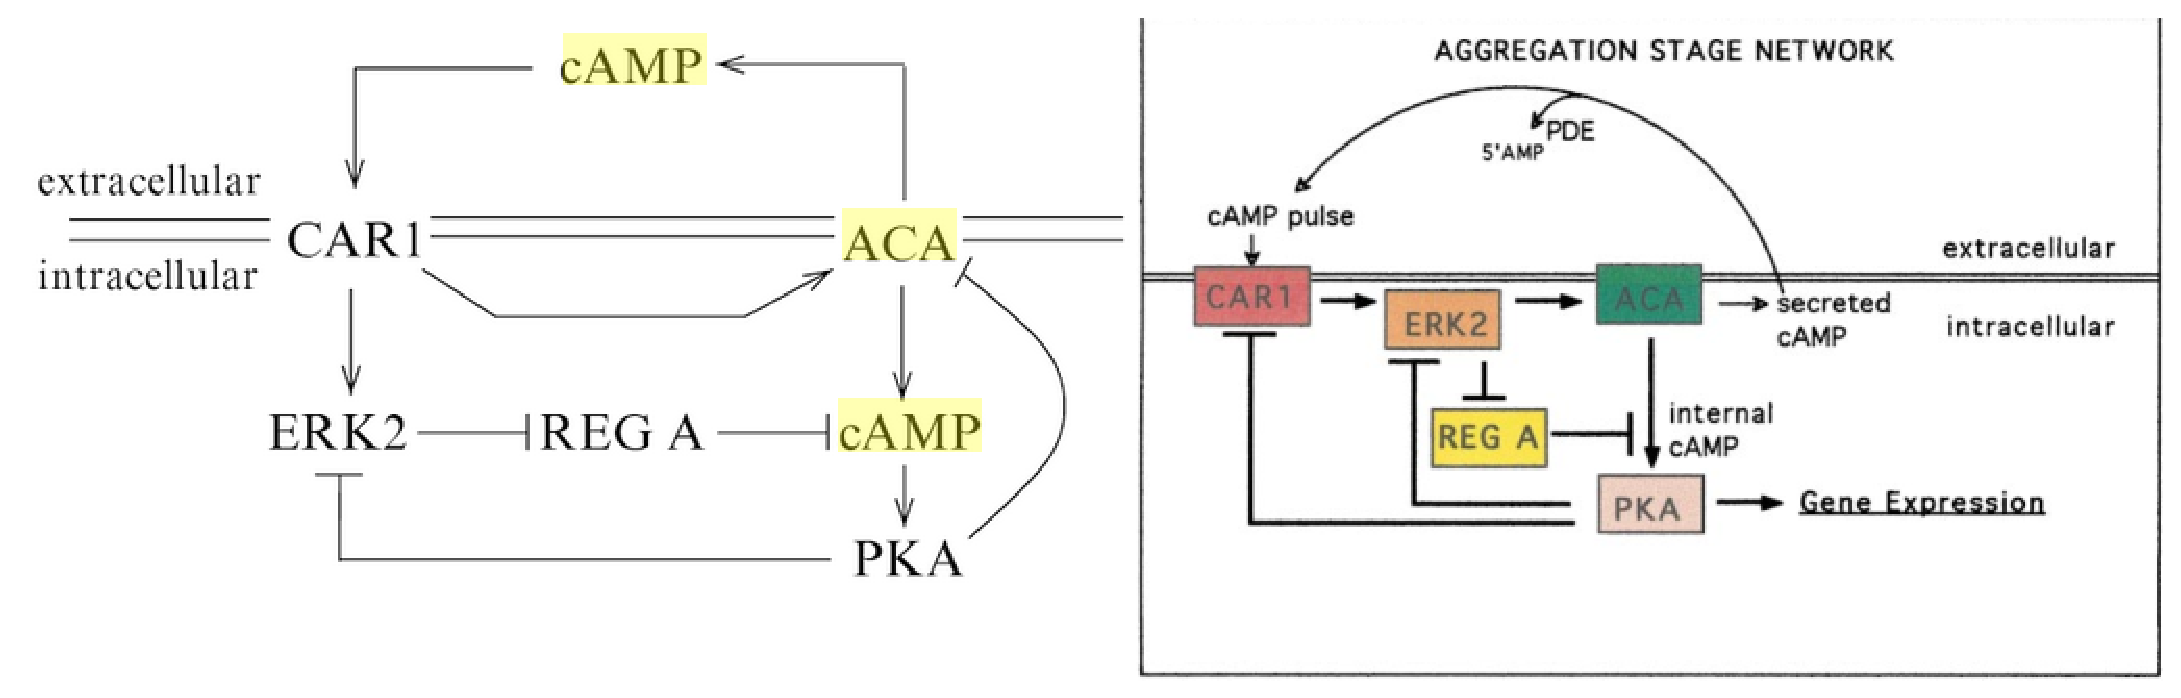
\includegraphics[height=3cm]{./images/cAMP-oscillation-Dictyostelium.eps}}
 \caption{Model of cAMP oscillation}
\label{fig:cAMP-oscillation-Dictyostelium}
\end{figure}

Model of the {\bf oscillation of intracellular cAMP level for Dictyostelium} was
first proposed by Michael Laub and William Loomis (1998) with a periodicity of 7
minutes, Fig.\ref{fig:cAMP-oscillation-Dictyostelium}. 

\begin{itemize}
  \item \textcolor{red}{Positive feedback}:
  \begin{enumerate}
  \item  extracellular cAMP binds to surface receptor CAR1 (Sect.\ref{sec:CAR1})
  
  activated CAR then cause  adenylyl cyclase (ACA) and the MAP kinase ERK2 
  transiently activated; each however function oppositely in terms of regulating
  cAMP
  
  \item activated ACA produces intracellular cAMP

  \end{enumerate}

  \item \textcolor{red}{Negative feedback}: 2-3 mins after the stimulation of
  cells with external cAMP and the activation of ACA, there is a rapid 5- to
  10-fold reduction in the affinity of CAR1  to  cAMP  and  a  consequent 
  reduction  in  ACA activity  (Caterina et al.,  1995a,b).  
  Thus, ligand binding oscillates in response to the levels of external cAMP.
  
  \begin{enumerate}

    \item A rise in the internal concentration of cAMP activates protein kinase
   A such that it inhibits ERK2 and leads to a loss-of-ligand binding by CAR1

    \item ERK2 phosphorylates the cAMP phosphodiesterase REG A that reduces the
  internal concentration of cAMP.
  
    \item After each peak (pulse), extracellular cAMP is rapidly hydrolyzed by a
  secreted PDE; whereas  intracellular  cAMP  is hydrolyzed by an intracellular
 phoshodiesterase (REG A)

  \end{enumerate}
%A secreted phosphodiesterase reduces external cAMP concentrations between
% pulses.
\end{itemize}
Experimental finding showed that cells become refractory to stimulus by
cAMP (e.g. adding exogenous cAMP) soon after responding to cAMP and then become
excitable again when the stimulus is removed.


The model is robust in that 25-fold changes in the kinetic constants linking the
activities have only minor effects on the predicted frequency. Moreover,
constant high levels of external cAMP lead to attenuation, whereas a brief pulse
of cAMP can advance or delay the phase such that interacting cells become
entrained.   


Maede (2004) showed spontaneous oscillations in activation of the
mitogen-activated protein (MAP) kinase ERK2 that occur in phase with peaks of
cAMP, and show that ERK2 modulates cAMP levels through the phosphodiesterase
RegA. Similar oscillatory processes may occur in cells of many different
species.

The robust circuit modeled here produces the spontaneous oscillations in cAMP
observed during the early development of D. discoideum and can account for the
synchronization of the cells necessary for chemotaxis and further development.



\subsection{-- function}
\label{sec:cAMP-function}

cAMP has been regarded as a freely diffusible second messenger that mediates the
action of a number of different receptors and modulates many cellular functions,
as diverse as cell (movements, growth, metabolism) and synaptic plasticity.
\begin{itemize}
  \item  {\bf In the heart}, cAMP is generated upon $\beta$-AR stimulation
  and is probably the most important modulator of sympathetic control over
  cardiac contractility by binding to different proteins.
  
  \item  The agent SKF 83822 is exclusively activates the cAMP pathway (Rashid
  et al., 2007) so it is used to study the functional role of cAMP.

  \item In 1970s, studies focused on cAMP's role in immune and inflammatory
  diseases: immunomodulatory properties of cAMP and the anti-inflammatory
  potential of PDE inhibitors (Lichtenstein et al.)

Also, during this time, the superfamily of PDE enzymes was born, as PDE
activities from tissue homogenate were found there exists pharmacokinetically
and biologically distinct PDE subtypes and that the relative amounts of these
PDEs varied among different tissues.
Then, the idea of using selective PDE inhibitors to target specific tissues,
pathways, and disease processes was first postulated (Sect.\ref{sec:PDE}).

  \item 
\end{itemize}


The important questions are: \textcolor{red}{Do cAMP/cGMP and their effectors
freely diffuse inside the cell or are they localized?} If they localize, do they
have any physiological or pathophysiological role? \citep{fischmeister2006}.


\begin{enumerate}
  \item the predominant downstream effector of cAMP is PKA - (Sect.\ref{sec:PKA}).

Most of cAMP effect on cell's function is via protein phosphorylation of PKA.
However, PKA is largely compartmentalized by an anchoring protein name AKAPS
(A-kinase anchoring proteins) - Sect.\ref{sec:AKAP}.  
   
  \item  
  \item 
\end{enumerate}


Other than the theory of cAMP local generation, the localization of effectos
like PKA can also affect the functional role of cAMP. In other words, there have
been some evidences that these proteins are not uniformly distributed
\begin{enumerate}
  \item Gs heterotetrameric guanine nucleotide-binding proteins [8]
  \item Adenylyl cyclases (AC) [8.9]
  \item AKAP-anchored PKA [10]
  \item L-type $\Ca$ channels: [9]
  \item Phosphodiesterases (PDE) \citep{Dodge2001} (Sect.\ref{sec:PDE}):
  localize to specific subcellular domains via binding to AKAP.
  
  In striatum, we focus on PDE10A (Sect.\ref{sec:PDE10})
\end{enumerate}
This provides potential anatomical basis for the local generation of cAMP.





\subsection{cGMP}
\label{sec:cGMP}

Both cAMP and cGMP are second messengers
within cells. \citep{Ashmana1963} found both cAMP and cGMP in rat urine.
Compared to cAMP, cGMP has a lower concentration, and thus is believed to play a
lesser role in cell function. As cGMP is hydrolized by PDE10
(Sect.\ref{sec:PDE10}), the level of PDE10A is important in regulating cGMP
function. 
\begin{itemize}
  \item  cGMP is measured using a cGMP enzyme immunoassay (EIA) kit (Cat No.
  581001, Cayman Chemical, Ann Arbor, MI)
\end{itemize}


The physiological role of cGMP has been found recently on
\begin{itemize}
  \item retina: cGMP mediates the effect of light on cation channels
  \item cGMP inhibits specific forms of PDE
\end{itemize}




\section{cAMP-regulated guanine nucleotide exchange factors (cAMP-GEFs, Epacs)}
\label{sec:cAMP-GEF}
\label{sec:Epacs}

cAMP-regulated guanine nucleotide exchange factors (cAMP-GEFs) are also called
exchange proteins directly activated by cAMP (Epacs).



\section{GAD (Glutamic Acid Decarboxylase)}
\label{sec:GAD}
\label{sec:GAD-enzyme}
% \label{sec:Glutamate-decarboxylase}
% \label{sec:GAD-Glutamate-decarboxylase}

Glutamic Acid Decarboxylase (GAD) is an enzyme that catalyzes the
decarboxylation of glutamate to GABA and CO2 (Sect.\ref{sec:GABA}).

\begin{verbatim}
Glutamate  ---[GAD]----> GABA  +  CO2
\end{verbatim}

In mammals, GAD exists in two isoforms encoded by two different genes - GAD1 and
GAD2. 
\begin{enumerate}

  \item  GAD1 (or GAD67 due to 67 kDa ): expressed in GABAergic neurons in brain
  
  spread evenly throughout the cell; and is transcribed during early
  development, i.e. is needed throughout development for normal cellular
  functioning.
  
  \item GAD2 (or GAD65 due to 65 kDA): expressed in GABAergic neurons in brain
  and pancreas
  
  expressed localized to nerve terminals, i.e. suggest GAD65 
  synthesizes GABA for neurotransmission; and is not found during
  development, i.e. not needed until slightly later in development when synaptic
  inhibition is more prevalent.
  
  GAD65 forms a complex with Heat Shock Cognate 70 (HSC70), cysteine string
  protein (CSP) and Vesicular GABA transporter VGAT, which, as a complex, helps
  package GABA into vesicles for release during
  
  \item At least two more forms, GAD25 and GAD44 (embryonic; EGAD) are described
  in the developing brain. 
  
GAD25 is encoded by two alternative transcripts of GAD1, I-80 and I-86.

GAD44 is encoded by only I-80.  
\end{enumerate}

\textcolor{red}{SUMMARY}: GAD65 and GAD67 synthesize GABA at different locations
in the cell, at different developmental times, and for functionally different purposes.

\textcolor{red}{Regulartory mechanisms}:
\begin{itemize}
  \item GAD65 is activated by phosphorylation while GAD67 is inhibited by
  phosphorylation.
  
  \item GAD67 is phosphorylated at threonine 91 by protein kinase A (PKA), while
  GAD65 is phosphorylated, and therefore regulated by, protein kinase C (PKC).
\end{itemize}

\section{GRK}
\label{sec:GRK}

The G protein-coupled receptor kinase (GRK) interactome: Role of GRKs in
GPCR regulation and signaling \citep{Ribas2007}. 

\begin{enumerate}
  \item phosphorylate mGluR group I - Sect.\ref{sec:mGluR_group-1-phosphorylation}
\end{enumerate}

GRK1 and GRK2 are mediated by
\begin{enumerate}
  \item Ca(2+)/NCS-1 - Sect.\ref{sec:NCS-1}
\end{enumerate}


\section{IC50 and EC50}
\label{sec:IC50}
\label{sec:EC50}


While EC50 is the dose (concentration depending how the experiment is done)
required to induce a response 50\% of the maximum,
IC50 refers to the concentration of opposite effect, i.e. dose/concentration
required to achieve 50\% inhibition (of a biological or biochemical function)
when you already have some sort of binding or activity.
 
Example: In regulating adenylyl cyclase (Sect.\ref{sec:AC-IIIa}, IC50 Gi$\alpha$
for 50\% of maximal inhibition effect is 50-150nM {\it in vitro} EC50 (i.e.
effective concentration of G$\alpha$s that causes 50\% of maximal response) is
10-30 nM.

\section{IC50 vs. Ki}
\label{sec:Ki}

Unlike IC50 (Sect.\ref{sec:IC50}) which changes depending on the experiment Ki
is an absolute value and is often referred to as the inhibition constant of a
drug. 

Ki refers to the concentration of the drug (can be either an agonist or
antagonist it just has to compete competitively with your radioligand for the
receptor) which would occupy 50\% of the receptors if there was no radioligand
present.

\begin{equation}
 Ki=\frac{\text{IC50}}{(1+([L]/Kd))}
\end{equation}
where [L] is the concentration of the radioligand used and Kd is the
dissociation constant of the radioligand.

The lower the IC50 or Ki values are the more potent the drug is (so the greater
affinity it has for the receptor). NOTE: these values have nothing to do with
activity, just binding of a drug to a receptor.

NOTE:  Antagonists can bind to the receptor wiht high affinity but have no
efficay. {\bf Radioligand assays} only provide information on binding affinity,
they are not {\bf funtional assays} (they provide no information on the activity
of a ligand, only information on whether something is a ligand for a specific
receptor).   

\begin{verbatim}
Affinity = how tightly a substance binds to the receptor

Efficacy = measurement of the maximum biological response of a compound

Potency = Amount of drug needed to achieve a specific biological response
\end{verbatim}


\section{Protease: cathepsin}
\label{sec:protease}
\label{sec:cathepsin}

NOTE: proteases are divided based on their pH-dependent activities
\begin{itemize}
  \item {\bf cathepsins protease}: (found in lysosomes) activated at the low pH
  found in lysosomes.

The activities mainly lies almost entirely within lysosome organelles.
There are, however, exceptions such as cathepsin K, which works extracellularly
after secretion by osteoclasts in bone resorption.

Depending on the amino acid at which the target protein is cleaved, the protease
are given the associated names, e.g. Cathepsin A (serine protease)

\url{https://en.wikipedia.org/wiki/Cathepsin}

  \item (calcium-activated) {\bf neutral protease} (calpain):
  intracellular cysteine protease not associated with the lysosome and having an
  optimum activity at neutral pH - Sect.\ref{sec:calpain}).
  
\end{itemize}

\section{PTEN}
\label{sec:PTEN}

{\bf Phosphatase and tensin homologue deleted on chromosome 10} (PTEN) is a
phosphatidylinositol phosphate phosphatase and is frequently inactivated in
human cancers. 

\subsection{PTEN upregulation}
\label{sec:PTEN-high-level}

High level of PTEN is harmful
\begin{enumerate}
  \item PTEN level is high in HD mouse model - Sect.\ref{sec:HD-theory-impaired-TrkBR-signaling}
  
  \item neonatal repeated exposures to isoflurane resulted in the activation of
  PTEN in the hippocampus; which decrease of self-renewal capacity in
  hippocampal neural precursor cells.
  
\end{enumerate}

\subsection{PTEN function}
\label{sec:PTEN-function}

PTEN is a phosphatase that inactivates Akt (Sect.\ref{sec:Akt-protein-kianse-B})

The balance between phosphoinositide 3-kinase (PI3K) and PTEN determines
PI(3,4,5)P3 levels - Sect.\ref{sec:PIP3}. 
PTEN dephosphorylates PIP3, and suppresses the growth and proliferation of many
cell types.  PTEN will convert PIP3 to PIP2 which limits cell
growth and proliferation. It has been heavily studied, in large part due to its
status as a tumour suppressor in many tumour types.

PI3K is regulated by a variety of intracellular and extracellular signals, but
little is known about the regulation of PTEN (review: Gericke et al., 2006).


The treatment of PTEN inhibitor BPV (pic) restored PSD-95 synthesis.
In addition, BPV (pic) treatment reversed the activation of NR2B-containing
NMDARs - found in thalamus; indicating a possible role of NR2B as the downstream
of PTEN in mediating tau phosphorylation in the neonatal rats repeatedly exposed
to isoflurane.  This can be a  novel role of PTEN in mediating tau
phosphorylation and cognitive deficits caused by neonatal repeated exposures to
isoflurane (Tan et al., 2017).



\chapter{EC4 enzymes}
\label{chap:EC4-enzymes}

\section{Adenylyl Cyclase (AC) (EC4.6.1.1)}
\label{sec:AC_adenylyl_cyclase}
\label{sec:adenylyl_cyclase}

{\bf Adenylyl cyclase} (AC, adenylate cyclase)  is an enzyme 
belonging to EC 4 family (Sect.\ref{sec:EC_4}).  The best known class of
adenylyl cyclases is class III or AC-III.

\subsection{classes: AC-I to AC-VI}
\label{sec:adenylyl-cyclase-classes}

There are 6 known classes of AC (I-VI) of no sequence similarities, i.e. it may
be explained by the product of convergent evolution. The best known and abundant
is a type of cAMP-producing enzyme - AC class III (AC-III), especially
AC-IIIa subclass, due to their important roles in human health
(Sect.\ref{sec:AC-III}).


\begin{enumerate}
  \item AC-I : (the first to be characterized) only found in {\it E. Coli} -
  $\gamma$-proteobacteria.

  \item AC-II: toxins secreted by  pathogenic bacteria such as Bacillus
  anthracis and Bordetella pertussis into host cell 

There is no known intracellular role of AC-II in these bacteria.

  \item AC-III: found in human and some bacteria. \textcolor{red}{We only focus
  on this} (Sect.\ref{sec:AC-III}).
  
Class III ACs are universal. They are found in metazoa, protozoa, fungi,
eubacteria, some archaebacteria and certain green algae.

  \item AC-IV: first reported in the bacterium Aeromonas hydrophila
  \item AC-V: reported in specific bacteri
  \item AC-VI: reported in specific bacteri
\end{enumerate}

\subsection{AC I}

Class I AC's are large cytosolic enzymes (~100 kDa) with a large regulatory
domain (~50 kDa) that indirectly senses glucose levels.

As a second messenger, upon activated, AC I activates expression of genes for
importing and metabolizing other sugar. cAMP exerts this effect by binding the
transcription factor CRP, also known as CAP.

\subsection{AC II}

AC II are toxins secreted by some bacterias.
These bacteria also secrete proteins that enable the AC-II to enter host cells,
where the exogenous AC activity undermines normal cellular processes.



\section{--  AC-III}

Class III ACs is a type of adenylyl cyclase - Sect.\ref{sec:adenylyl_cyclase})
that are most related to human's health. They are considered as universal, as
they are found in metazoa, protozoa, fungi, eubacteria, some archaebacteria and
certain green algae.


\subsection{cellular localization}

Most AC-III's are integral membrane proteins involved in transducing
extracellular signals into intracellular responses.


\subsection{functions}

\begin{verbatim}
extracellular ligand --> GPCR --> G-protein --> AC ---[ATP]--> cAMP 
\end{verbatim}

\begin{enumerate}
  \item {\bf in human liver}: adrenaline (via GPCR) indirectly stimulates AC to
  mobilize stored energy in the "fight or flight" response. 
  
  Nobel Prize was awarded to Earl Sutherland in 1971 for this discovery.
  
  The outside signal (in this case, adrenaline) binds to a receptor (which is a
  GPCR), which transmits a signal to the G protein, which transmits a signal to
  adenylyl cyclase, which transmits a signal by converting adenosine triphosphate to
  the second messenger cAMP - Sect.\ref{sec:cAMP}.
  
  \item 
\end{enumerate}

\subsection{activator/inhibitor}

\textcolor{red}{All classes of AC catalyzes the conversion from ATP to cAMP,
and also create pyrophosphate} (i.e. $\ce{P2O7^{4-}}$ or abbreviated as PP$_i$)
- Sect.\ref{sec:pyrophosphate}
\begin{verbatim}
ATP -----[AC]------>  cAMP + (PO4-PO3)^{4-}
\end{verbatim}

\begin{itemize}

  \item activated by released G$_s\alpha$ subunit (Sect.\ref{sec:Gs-protein})
  via the stimulation of catecholamine - Sect.\ref{sec:Catecholamines}
  
  \item inhibited by released G$_i$ subunit (Sect.\ref{sec:Gi-protein})

\end{itemize}
besides other AC-class-specific activator/inhibitor to be discussed in each
subsection.


\begin{mdframed}
NOTE: there are {\bf photoactivable adenyly cyclase} (PAC) found in {\it E.
gracilis}, and can be inserted into other organisms via genetic manipulation,
which is a useful technique for neuroscience researchs.
\end{mdframed}

\subsection{AC-III: a, b, c, d}
\label{sec:AC-III}
\label{sec:adenylyl-cyclase-classIII}

Class III adenylyl cyclases is the most abundant type of
AC (Sect.\ref{sec:AC_adenylyl_cyclase}).  
\begin{itemize}
  \item sequence - Sect.\ref{sec:AC-III-sequence}
  \item classification - Sect.\ref{sec:AC-III-classification}
\end{itemize}

\subsection{-- sequence/structure/isoforms}
\label{sec:AC-III-sequence}
\label{sec:AC-III-catalytic-domains}
\label{sec:AC-III-classification}

Most AC-III are transmembrane protein with 12 transmembrane (TM)
segments, organized in the following order:

{\bf N-terminal - M1 region (6 TMs) - C2 cytoplasmic domain - M2 region (6
  TMs) - C1 cytoplasmic domain}.

The important parts for functions are N-terminal, C1 and C2 regions.
NOTE: The two cytoplasmic regions (C1a and C2a) are the active sites (i.e.
catalytic sites or catalytic domain - (termed {\bf cyclase homology domain
(CHD)})). The catalytic sites must form dimer for the AC to be active, and the
catalytic process occurs at the dimer interface.

\begin{enumerate}
  \item C1 region is divided into C1a and C1b
  \item C2 region is divided into C2a and C2b
\end{enumerate}

The  first  class  III  AC  was  cloned  from {\it Saccharomyces cerevisiae}.

The catalytic domains are quite divergent in their primary structures and have
been subdivided into four subclasses (class IIIa - class IIId): ACIIIa, ACIIIb,
ACIIIc, and ACIIId \cite{linder2003}. \textcolor{red}{Subclass a (ACIIIa) is the
one found in mammals} (Sect.\ref{sec:AC-IIIa}).

%Most class III adenylyl cyclases are multi-domain proteins.

\subsection{-- regulators}
\label{sec:AC-III-regulator}

The catalytic domains (cyclase homology domain (CHD)) of class III ACs must form
dimers to be active.

Activated AC class III catalyze the conversion from adenosin triphosphate (ATP -
Sect.\ref{sec:ATP-molecule}) to produce cAMP - (Sect.\ref{sec:cAMP}) and
pyrophosphate (Sect.\ref{sec:pyrophosphate}).
Also, this process requires divalent cations, usually $\Mg$.
\footnote{\url{http://www.ncbi.nlm.nih.gov/books/NBK27958/}}
\begin{equation}
\text{(excess)} \ce{ATP ->[\text{(activated)AC}][\text{(required cofactor)}
\Mg] cAMP + pyrophosphate}
\end{equation}


\subsection{AC-IIIa (mammals): 12 TM}
\label{sec:AC-IIIa}

AC-IIIa has 10 known isoforms: AC1-AC10 (AC type I to AC type X) or
ADCY1-ADCY10.

\begin{itemize}
  \item membrane-bound AC: 9 isoforms (type I to IX) 

In the membrane-bound AC, the two CHDs: C1a and C2 are tethered to the membrane
anchors: M1 and M2. A chimeric catalyst composed of type V AC C1a and type AC C2
in complex is mainly used to study the function of AC-III.
  
  \item soluble AC: 1 isoform (sAC)
\end{itemize}

\subsection{-- regulators}
\label{sec:ACIII-regulators}

Remember that AC-IIIa has 10 isoforms in which 9 isoforms are membrane-bound
(Sect.\ref{sec:AC-III-sequence}).

The activity of the nine membrane-bound AC isoforms is differentially modulated
by a complex set of primary and secondary regulators, Fig.\ref{fig:AC-III-a}
(review: Linder - Schultz 2006):

\begin{enumerate}
  
  \item {\bf primary regulator} Gs$\alpha \cdot$ GTP or pharmacological agents
  (e.g.  forskolin):
  stimulate all 9 isoforms by a factor of 3 to 20
  %Gs and forskolin: enhance AC-III
  
  Upon G-protein binding, the dissociation constant (Kd) of V C1a/II C2 drops
  from $> 5\muM$ to 0.7 $\muM$.

In tissues that expresses both AC5 and AC6 (e.g. cardiac fibroblasts, gastric
smooth muscle) or transfected cells to express both (HEK-AC5 and HEK-AC6 cells),
G$\alpha$q enhances activity of AC6 activity; but not AC5.

  \item {\bf primary regulator} $\Ca$/Calmodulin: stimulate AC3, AC5, and AC8
  
    
  \item {\bf secondary regulator} (non-competitive antagonist) Gi and
  G$\beta\gamma$: inhibit AC-III (mostly in AC1, AC5 and AC6; and much lesser in
  other isoforms)
  
Gi$\alpha1$, Gi$\alpha2$, Gi$\alpha3$, Go$\alpha$, Gz$\alpha$ acts as secondary
regulator, i.e. \textcolor{red}{do not inhibit the basal activity of AC; but
only activity stimulated} by physiological regulators such as G$\alpha$s (above)
or pharmacological agents such as forskolin.

For AC-III type V and type VI: Gi$\alpha$ inhibited 70-80\% the enhancement
caused by G$\alpha$s (IC50 Gi$\alpha$ for 50\% of maximal inhibition effect is
50-150nM {\it in vitro}).  {\bf NOTE}: Go$\alpha$ has no inhibition effect on
these.

For AC-III type I: all Gi$\alpha$ and Go$\alpha$ inhibited 50\% the enhancement
caused by $\Ca$/Calmodulin; but not the enhancement caused by G$\alpha$s.

  \item G$\beta\gamma$: with a complex pattern
  
  \begin{enumerate}
    \item secondary or 'conditional' regulator on AC-II, AC-IX,
    AC-VI 
    
G$\beta\gamma$ increase AC-II activity with a weak 1.5x enhancement only.
 
 NOTE: G$\alpha$s increase 4- to 11-fold with EC50 (i.e. effective
 concentration of G$\alpha$s that causes 50\% of maximal response) is 10-30 nM.

    \item inhibit AC-I, AC-III, and AC-VIII.
    
G$\beta\gamma$ causes maximum 
\begin{itemize}
  \item 80\% inhibition on enhanced activity of AC-I
stimulated by $\Ca$/Calmodulin; with IC50 is 5-10 nM.

  \item 50\% inhibition on enhanced activity of of AC-I stimulated by G$\alpha$s
  
  \item 30\% inhibition on enhanced activity of AC-I stimulated by forskolin.
\end{itemize}

  \end{enumerate}
  
  
  \item PKA phosphorylation (Sect.\ref{sec:PKA}):  inhibit AC5, AC6
  
  
  \item PKC phosphorylation: enhance AC5, inhibit AC6
  
PKC$\alpha$ and PKC$\zeta$ (Sect.\ref{sec:PKC}) enhances basal activity, 
as well as G$\alpha$s-mediated and forskolin-mediated enhanced activity, of
recombinant AC5, similar to AC2. However, there was one study confirmed that PMA
(phorbol ester) does not stimulate AC5. 

The effects of PKC phosphorylation on AC6 are inconsistent (can be inhibition,
stimulation or no effect). 
%https://books.google.com/books?id=UKUt23dBIDMC&pg=PA198&lpg=PA198&dq=PKA+phosphorylation:+inhibit+AC5,+AC6&source=bl&ots=23bENfFPjs&sig=0Z2uJin5YC71_06i-U056ijhRQA&hl=en&sa=X&ved=0ahUKEwiazOjh5dTQAhVJ6YMKHa6PCK8Q6AEILDAB#v=onepage&q=PKA%20phosphorylation%3A%20inhibit%20AC5%2C%20AC6&f=false


\end{enumerate}

As showed above, the mode of activation (either via G$\alpha$s or
$\Ca$/Calmodulin) is important for the effect of antagonists.

\begin{figure}[hbt]
  \centerline{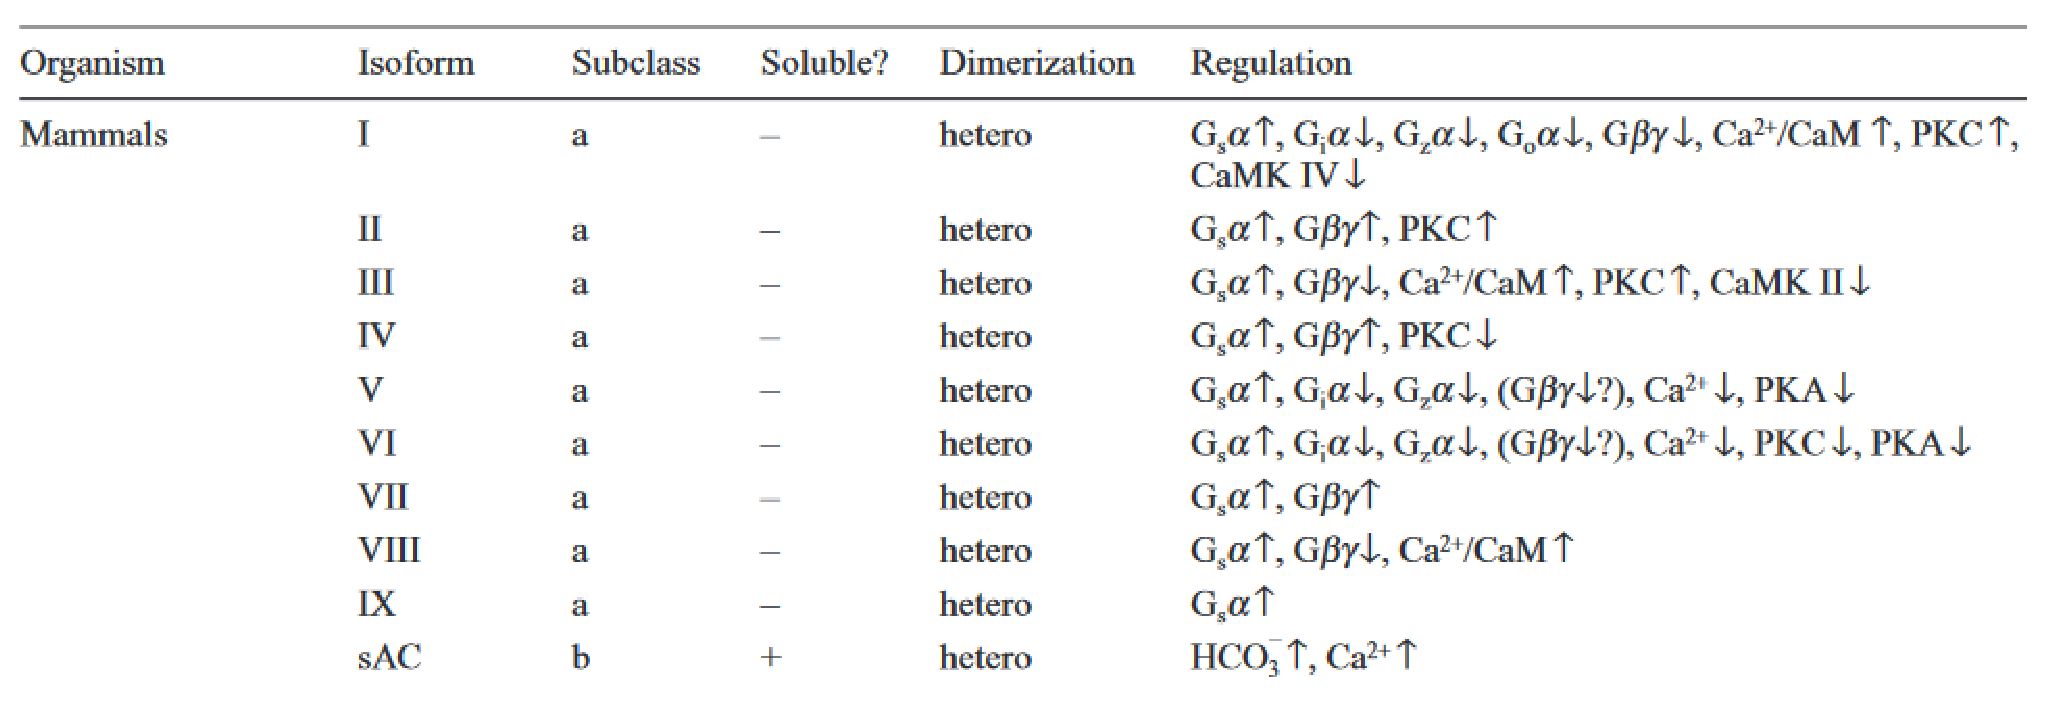
\includegraphics[height=4cm,
    angle=0]{./images/AC-III-a.eps}}
\caption{class III AC subclass a (in mammals)}
\label{fig:AC-III-a}
\end{figure}

\subsection{-- brains}

{\bf In neurons}
\begin{itemize}
  \item striatum: AC5 is the principal integrating  signals  from  multiple 
  receptors  including  D1, D2, and  $A_{2A}$ receptors in  striatum 
  \item 
\end{itemize}

$\Ca$-sensitive AC are located next to VDCC for faster reactions to $\Ca$
influx. These ACs are suspected to play an important role in learning process,
as a \textcolor{red}{coincidence detectors}
(Sect.\ref{sec:coincidence-detectors}).

\subsection{-- hearts}

{\bf In hearts}, AC5 and AC6 are the dominant isoforms; with AC7 and AC9 at mRNA
levels and AC4 both at mRNA and protein level \citep{fischmeister2006}.
It's impossible to discriminate AC5 from AC6 using current available antibodies.
So, immunofluorescence staining of isolated adult ventricular myocyte using a
common AC5/AC6 antibody showed that the signal from them with preferential
localization in T-tubular membrane \citep{fischmeister2006}.

\subsection{AC-IIIa type I}

Types I and VIII appear to be expressed exclusively in the brain,
adrenal gland and retina.

\subsection{AC-IIIa type V}
\label{sec:AC5}
\label{sec:AC-IIIa-type-V}

Type V adenylyl cyclase is highly enriched in brain and is localized largely to
the striatum and related structures, such as the nucleus accumbens and olfactory
tubercle, which are innervated by dopamine. It is inhibited by free Ca2+ at
physiological concentrations (0.1 to 1.0 $\muM$).
  
AC type V enzyme is also expressed in heart and kidney, where it is associated
with blood vessels; the anterior lobe of the pituitary; and the retina.


\subsection{AC-IIIa type VI}

Type VI adenylyl cyclase is enriched in brain and heart, with low
expression in other tissues, such as testes, muscle, kidney and lung.
  
Type VI adenylyl cyclase is structurally similar to the type V enzyme, and
both are inhibited by free Ca2+ at physiological concentrations (0.1 to 1.0
$\muM$)

  
\subsection{AC-IIIa type VII}

Type VII adenylyl cyclase is found in several tissues; concentrations are
highest in lung and spleen, moderate in heart and low in brain, kidney and
skeletal muscle

\subsection{AC-IIIa type IX}
  
Type IX: Less is known about the type IX enzyme, which to date has not
been characterized extensively; yet the most divergent in sequence of AC-III
isoforms. 

White-type (WT) AC9 is insensitive to forskolin; yet replacing a single amino
acid (Y1021L) in C2 loop can restore forskolin sensitivity.

AC9 is stimulated by G$\alpha$s; and inhibited by $\Ca$/calcineurin.

Coincidence detector, i.e. G$\alpha$s-stimulated AC9 activity (G$\alpha$s from
M1 receptor or 5HT$_{2A}$ - Sect.\ref{sec:M1-muscarinic-receptor} and
Sect.\ref{sec:5-HT3-receptor}) is

\begin{itemize}

  \item inhibited by activation of G$\alpha$i/o-coupled receptors; and this
  inhibition is removed by pertussis toxin
  
  \item reduced by 50\% in the presence of phorbol esters (appear to be the
  result of activation of a novel PKC isoforms; which is blocked by
  bisindolylmaleimide I; but not the conventinal PKC isoforms blockers - Go6976
  - Sect.\ref{sec:PKC}).
  
\end{itemize} 


\section{Guanyl cyclase (GC) (EC4.6.1.2)}
\label{sec:guanylate-cyclase}

Guanylate cyclase (guanyl cyclase, guanylyl cyclase, or GC)
is a lyase enzyme


\section{Guanine nucleotide}
\label{sec:guanine-nucleotide}

Nucleotides are small molecules composed of three parts, a nitrogenous base, a
sugar and one or more phosphates. Guanine nucleotide
\begin{enumerate}
  \item GTP

\begin{verbatim}
-(PO3)-(PO3)-(PO3)-O-(sugar)-Base
\end{verbatim}

  \item GDP

\begin{verbatim}
-(PO3)-(PO3)-O-(sugar)-Base
\end{verbatim}
Guanosine diphosphate (GDP) has only two phosphate groups.

\end{enumerate}
The nucleotide GTP are hydrolyzable by GAF (Sect.\ref{sec:GAF-domain})

The nonhydrolyzable guanine nucleotides such as GTP$\gamma$S.


\section{Molecular switch}
\label{sec:molecular-switch}


\begin{enumerate}
  \item G-proteins - Sect.\ref{sec:G-protein}
  
  \item DARPP32 - Sect.\ref{sec:DARPP32}: molecular switch to regulate and
  fine-tunes the phosphorylation state of PP-1.

NOTE: DARPP32, once activated, is a potent inhibitor of PP-1.
  
  \item DNA topoisomerase II$\beta$: molecular switch in neural differentiation
  of mesenchymal stem cells
  \url{https://www.ncbi.nlm.nih.gov/pubmed/25217229}
  
  \item notch signaling pathway (originally discovered in Drosophila): 
  \url{https://www.ncbi.nlm.nih.gov/pubmed/20681026}
  
  \item 
\end{enumerate}